%----------------------------------------------------------------------------------------
%    PACKAGES AND THEMES
%----------------------------------------------------------------------------------------

\documentclass[aspectratio=169,xcolor=dvipsnames]{beamer}
\usetheme{SimplePlus}

\usepackage{MnSymbol,bbding,pifont}
\usepackage{hyperref}
\usepackage{graphicx} % Allows including images
\usepackage{booktabs} % Allows the use of \toprule, \midrule and \bottomrule in tables
\usepackage{tcolorbox}
\usepackage{outlines}
\usepackage{tikz}
\usepackage{listings}
\usepackage{caption}
\lstset{basicstyle=\ttfamily, keywordstyle=\bfseries}

\renewcommand{\u}[1]{\textcolor{red}{#1}}
\renewcommand{\k}[1]{\textcolor{blue}{#1}}
\newcommand{\flag}{\tikz[baseline=-0.5ex, scale=0.15]{\draw[thick] (0,0) -- (0,3); \fill[red] (0,2.5) -- (2,2) -- (0,1.5) -- cycle;}}

\usepackage{rotating}	%% introduce sideways env

%% Public TikZ libraries
\usetikzlibrary{positioning}
\usetikzlibrary{shapes}
\usepackage{algorithm2e}
\renewcommand{\thealgocf}{} 


%% Custom TikZ addons
\lstset{ 
  language=C,               % specify the language
  basicstyle=\ttfamily,      % basic font style
  keywordstyle=\color{blue}, % keyword color
  commentstyle=\color{green}, % comment color
  stringstyle=\color{red},   % string color
  frame=single,             % frame around the code
  breaklines=true,          % line breaking
  captionpos=b              % caption position at the bottom
}

%----------------------------------------------------------------------------------------
%    TITLE PAGE
%----------------------------------------------------------------------------------------

\title{Challenges FCSC 2025}
\subtitle{Cryptographie et Side Channel}

\author{St4ck0verfl0w}

\institute
{
	Redacted
}
\date{\today} % Date, can be changed to a custom date

%----------------------------------------------------------------------------------------
%    PRESENTATION SLIDES
%----------------------------------------------------------------------------------------

\begin{document}

%------------------------------------------------
%------------------------------------------------

\begin{frame}
    % Print the title page as the first slide
    \titlepage
\end{frame}

%------------------------------------------------
%------------------------------------------------

\begin{frame}{France Cyber Security Challenge (FCSC)}
    \begin{columns}[c]
        \column{.45\textwidth}
            \begin{center}                  
                
\includegraphics[width=0.8\textwidth]{img/meme/intro.png}
            \end{center}

        \column{.65\textwidth} % 
           \begin{itemize}
               \item  CTF organisé par l'\textbf{ANSSI} (individuel)
               \item Recrute l'équipe de France pour les championnats Européens
               \pause
               \item \textbf{10 jours d'épreuves} (18 au 27 mai), 99 challenges
                \item 10 catégories dont 6 classantes (\textbf{crypto, reverse, pwn, hardware, web, speerdun}, SCA, forensic, misc, intro)
                \pause
                \item 2046 inscrits (1848 ayant fait au moins une épreuve)
                \item \url{https://fcsc.fr} puis \url{https://hackropole.fr}
                \pause
                \item \textcolor{red}{Particularité cette année : le speedrun}
           \end{itemize}

    \end{columns}
        \pause
    \begin{tikzpicture}[overlay, remember picture]
        \node[rotate=23, scale=5, text=red] at (current page.center) {SPOILER ALERT};
    \end{tikzpicture}
\end{frame}

\begin{frame}{CTFd}
    \centering
    \only<1>{
        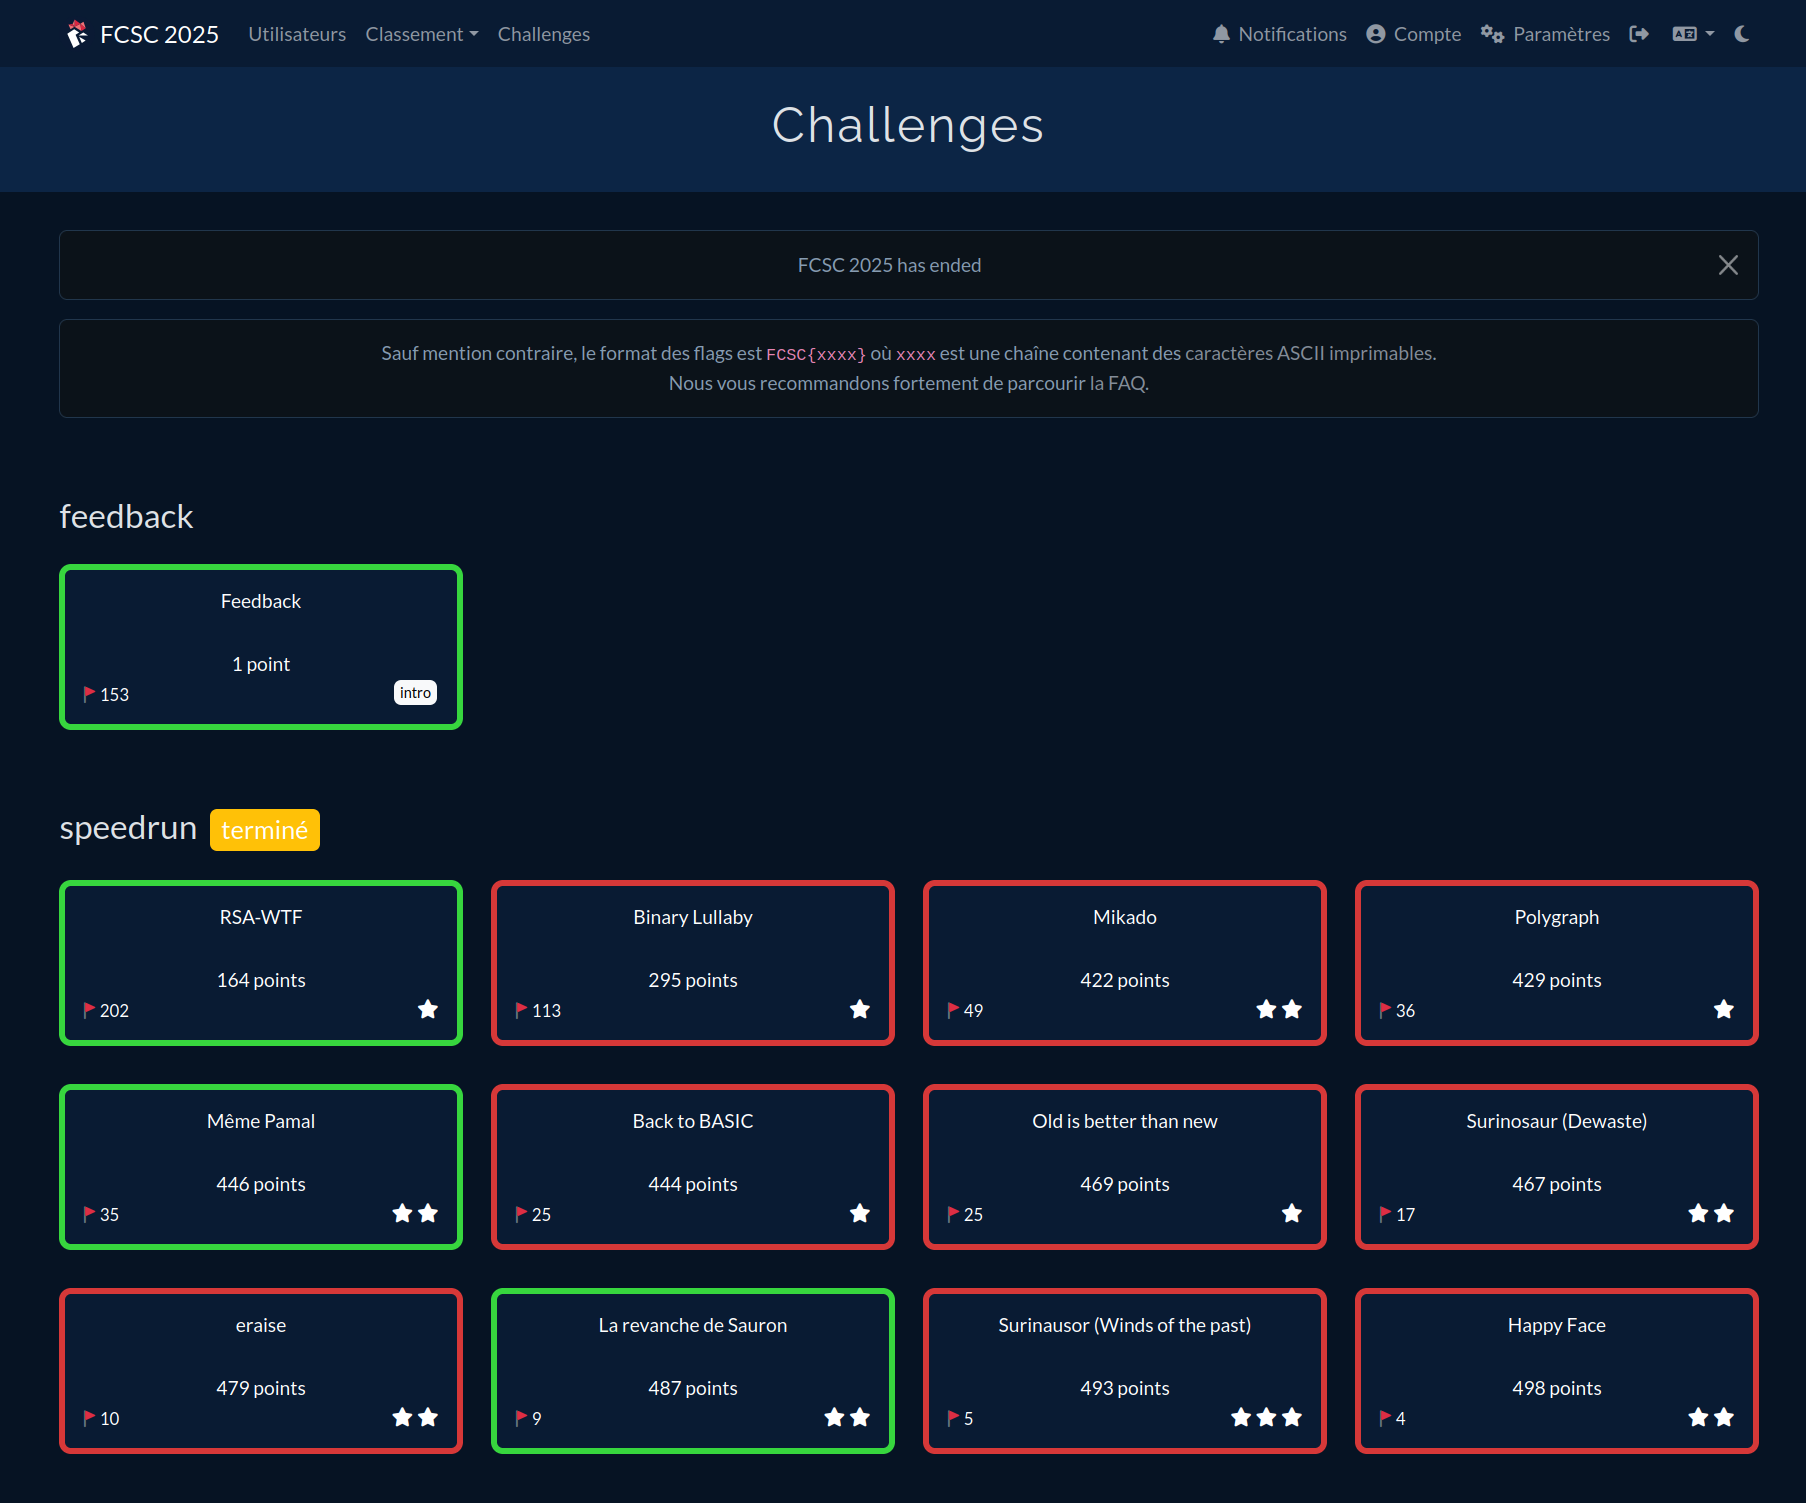
\includegraphics[width=0.6\textwidth]{img/fcsc-board.png}
    }   
    \only<2>{
        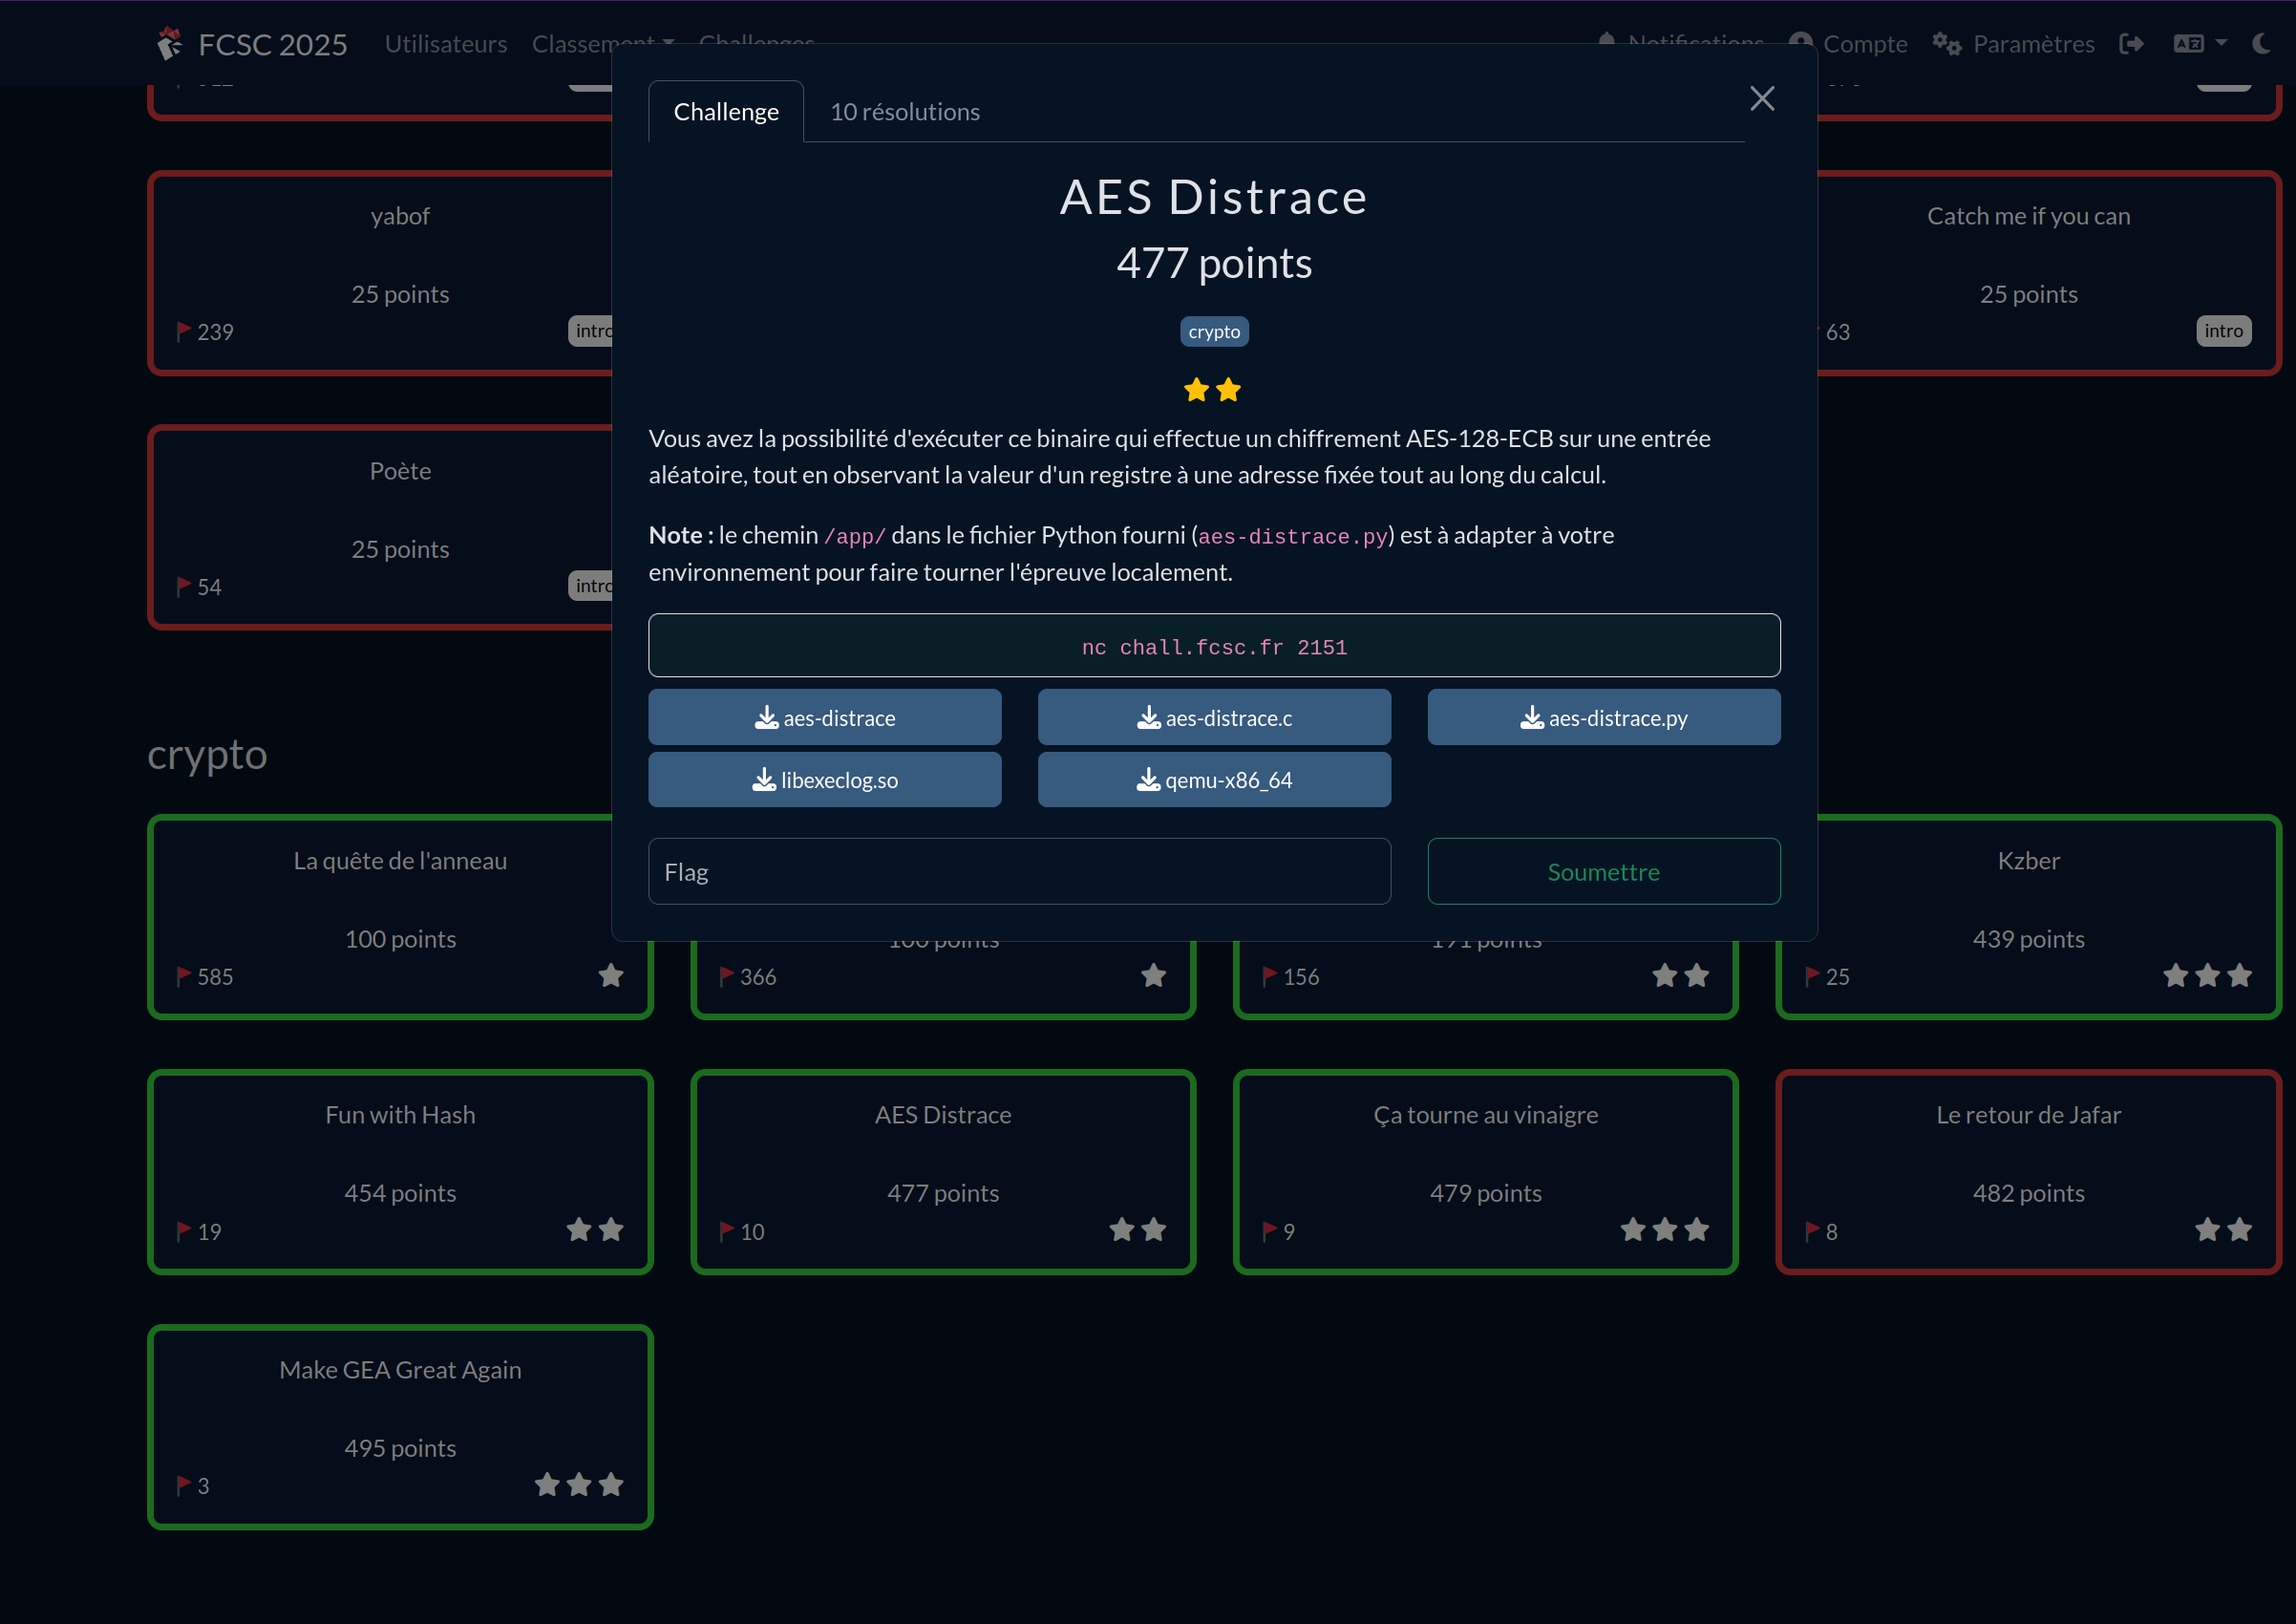
\includegraphics[width=0.7\textwidth]{img/exemple-chal.png}
    }   
    \only<3>{
    \begin{columns}[c]
        \column{.5\textwidth}
            \begin{center}                  
                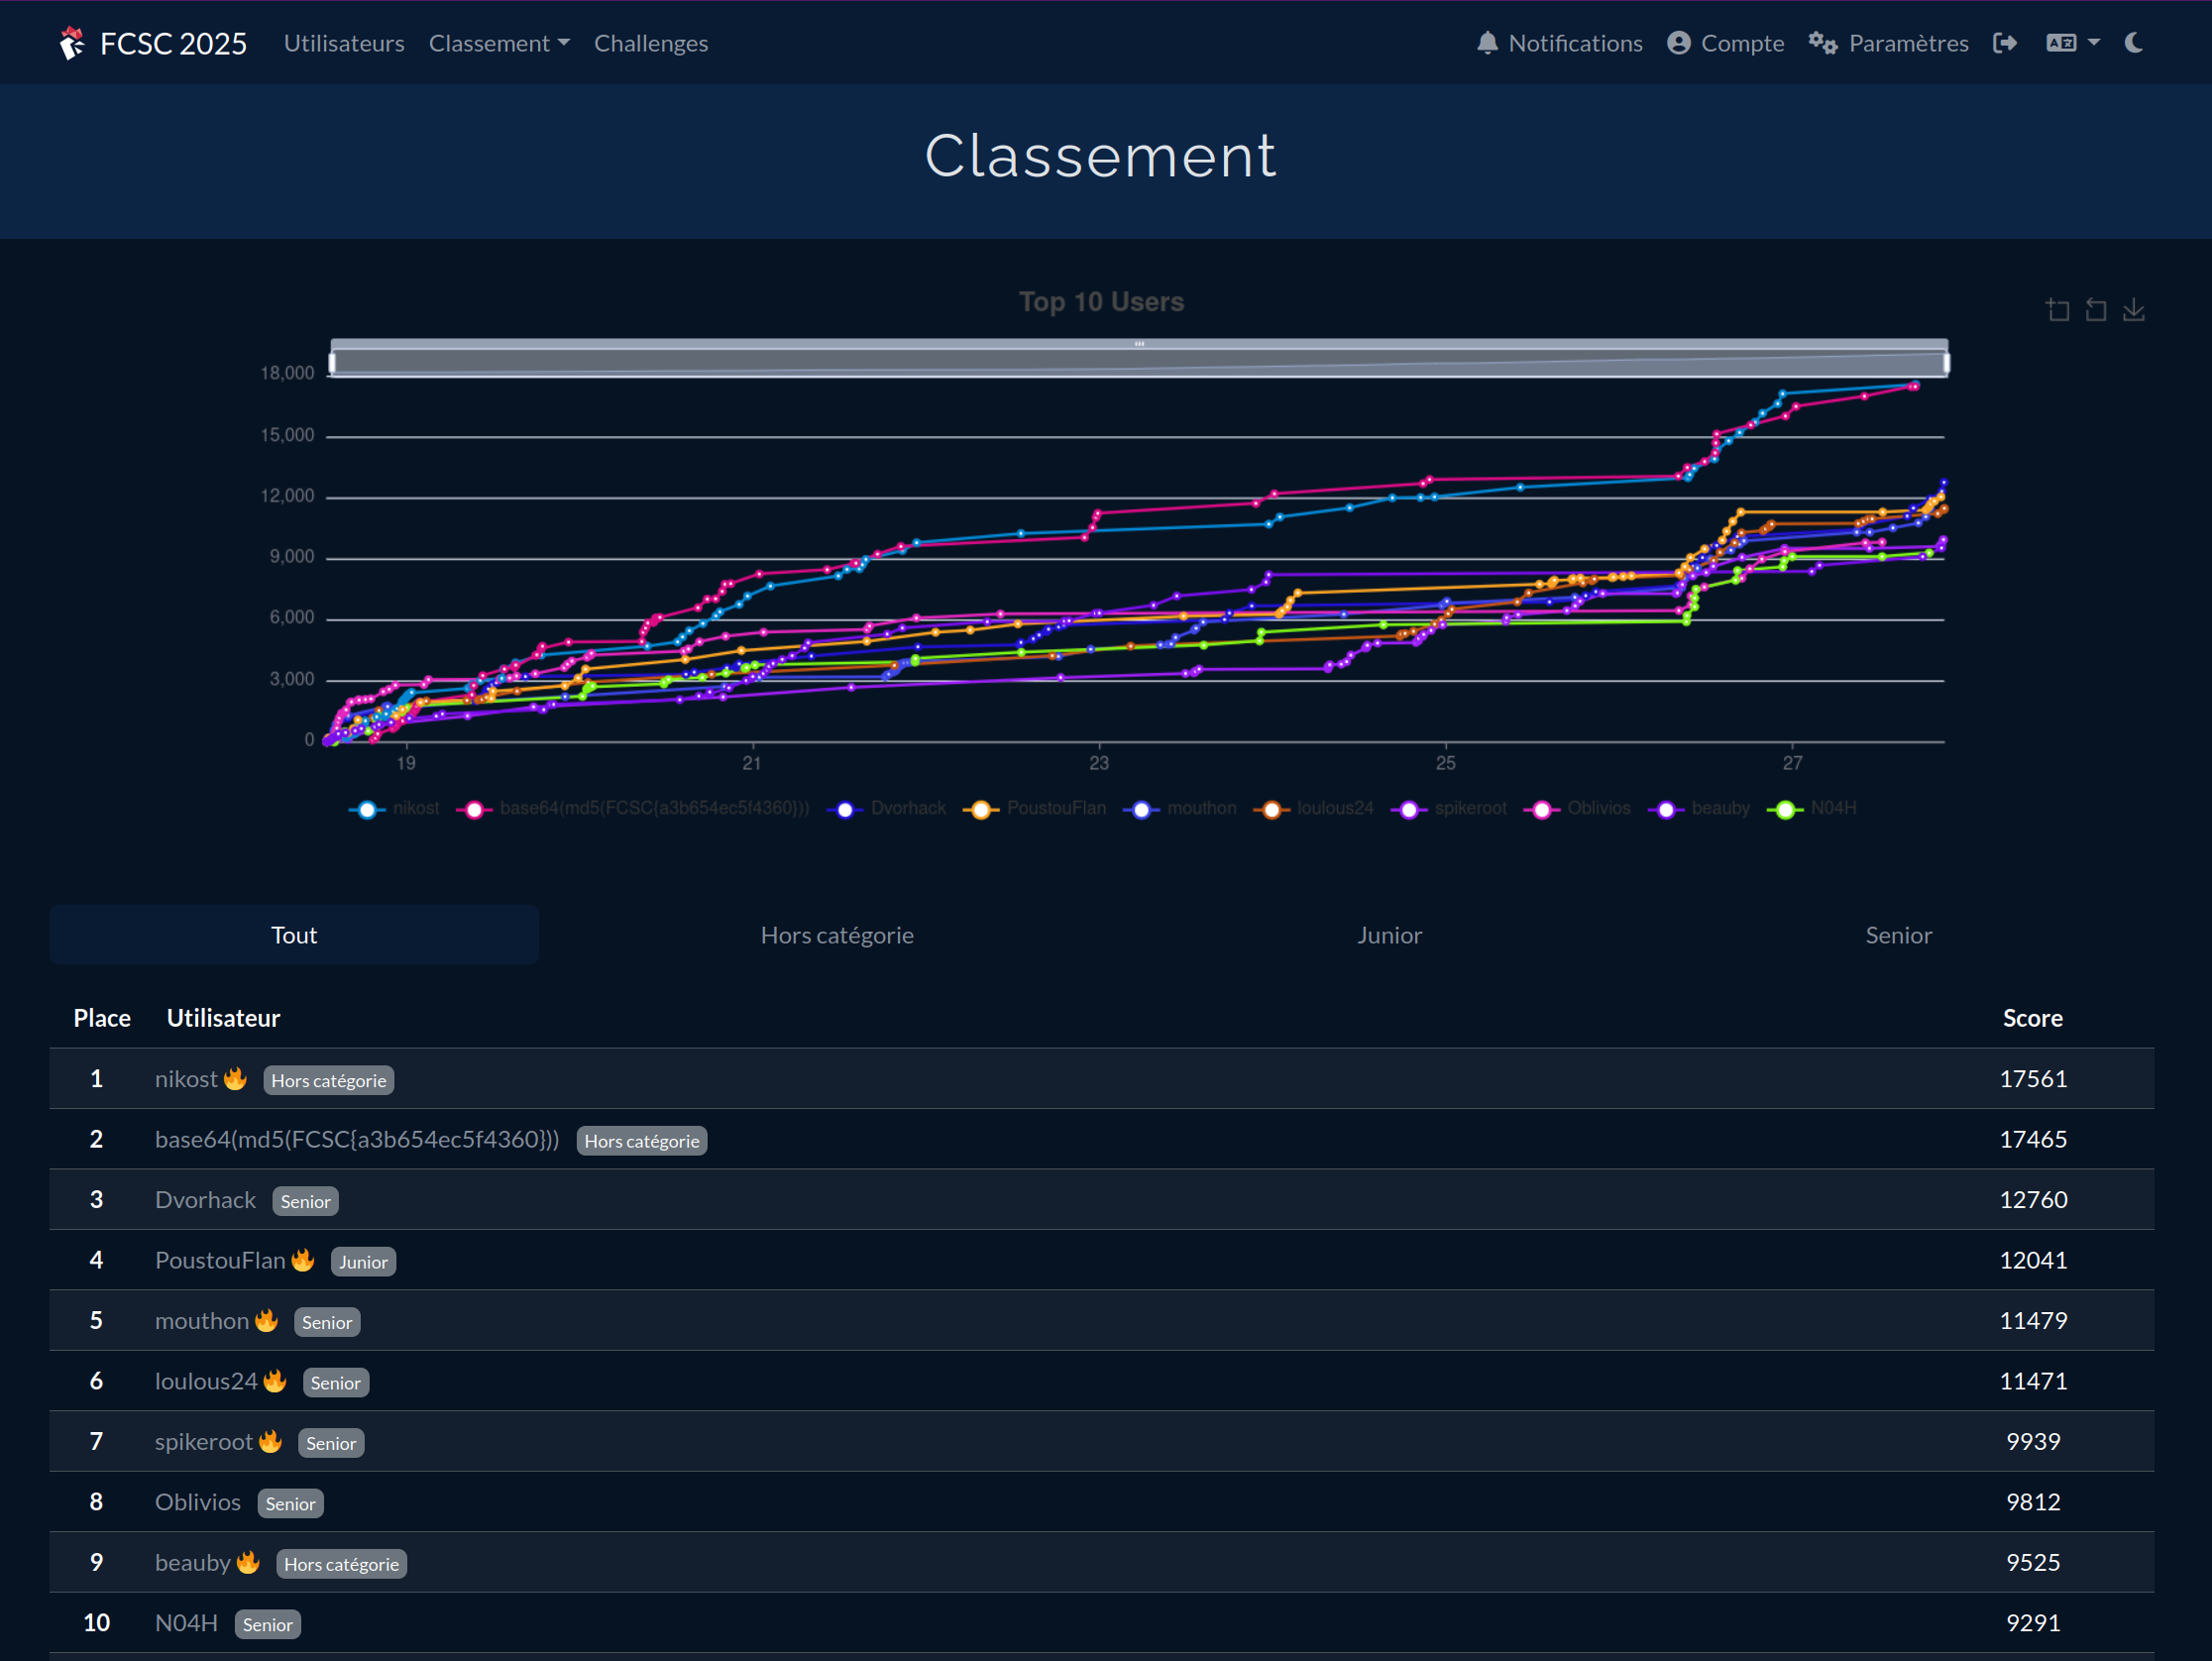
\includegraphics[width=1\textwidth]{img/classement.png}
            \end{center}

        \column{.5\textwidth} % 
            \begin{center}                  
                \includegraphics[width=1\textwidth]{img/top-catégorie.png}
            \end{center}
    \end{columns}
    }   
\end{frame}
%------------------------------------------------
%------------------------------------------------

\begin{frame}{Sommaire}
    % Throughout your presentation, if you choose to use \section{} and \subsection{} commands, these will automatically be printed on this slide as an overview of your presentation
    \tableofcontents
\end{frame}

%------------------------------------------------
%------------------------------------------------

\begin{frame}{Les vrais héros}
\centering

\includegraphics[width=0.5\textwidth]{img/meme/thanks.png}
\end{frame}


\section{Side-channel}
\subsection{Differential Power Analysis}
\begin{frame}{Differential Power Analysis}
    \large{\centerline{\textbf{Introduction au side channel}}}

\end{frame}

\begin{frame}{CryptoBro en détresse \FiveStar \hfill 138 résolutions}
    \begin{columns}[c]
        \column{.45\textwidth}
        \begin{center}                  
            
\includegraphics[width=0.8\textwidth]{img/meme/cryptobros.png}
        \end{center}

        \column{.65\textwidth} % 
           \begin{outline}
               \1 Objectif
                \2 Récupérer le PIN d'un portefeuille crypto

            \pause
               \1 Données
                \2 Une trace courant pour chaque PIN
           \end{outline}
    \end{columns}
\end{frame}


\begin{frame}{Faillock et bypass}
    \centering
    \only<1>{
        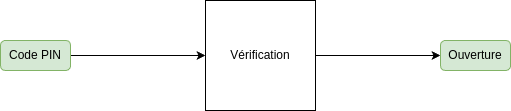
\includegraphics[width=0.6\textwidth]{img/sca/dfa/dfa-valid.drawio.png}
    }
    \only<2>{
        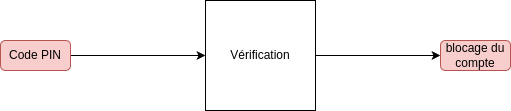
\includegraphics[width=0.6\textwidth]{img/sca/dfa/dfa-invalid.drawio.png}
    }
    \only<3->{
        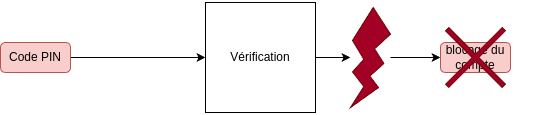
\includegraphics[width=0.6\textwidth]{img/sca/dfa/dfa-cutpower.drawio.png}
    }
\end{frame}

\begin{frame}{Comparaison séquentielle}
    \centering
    \only<1>{
        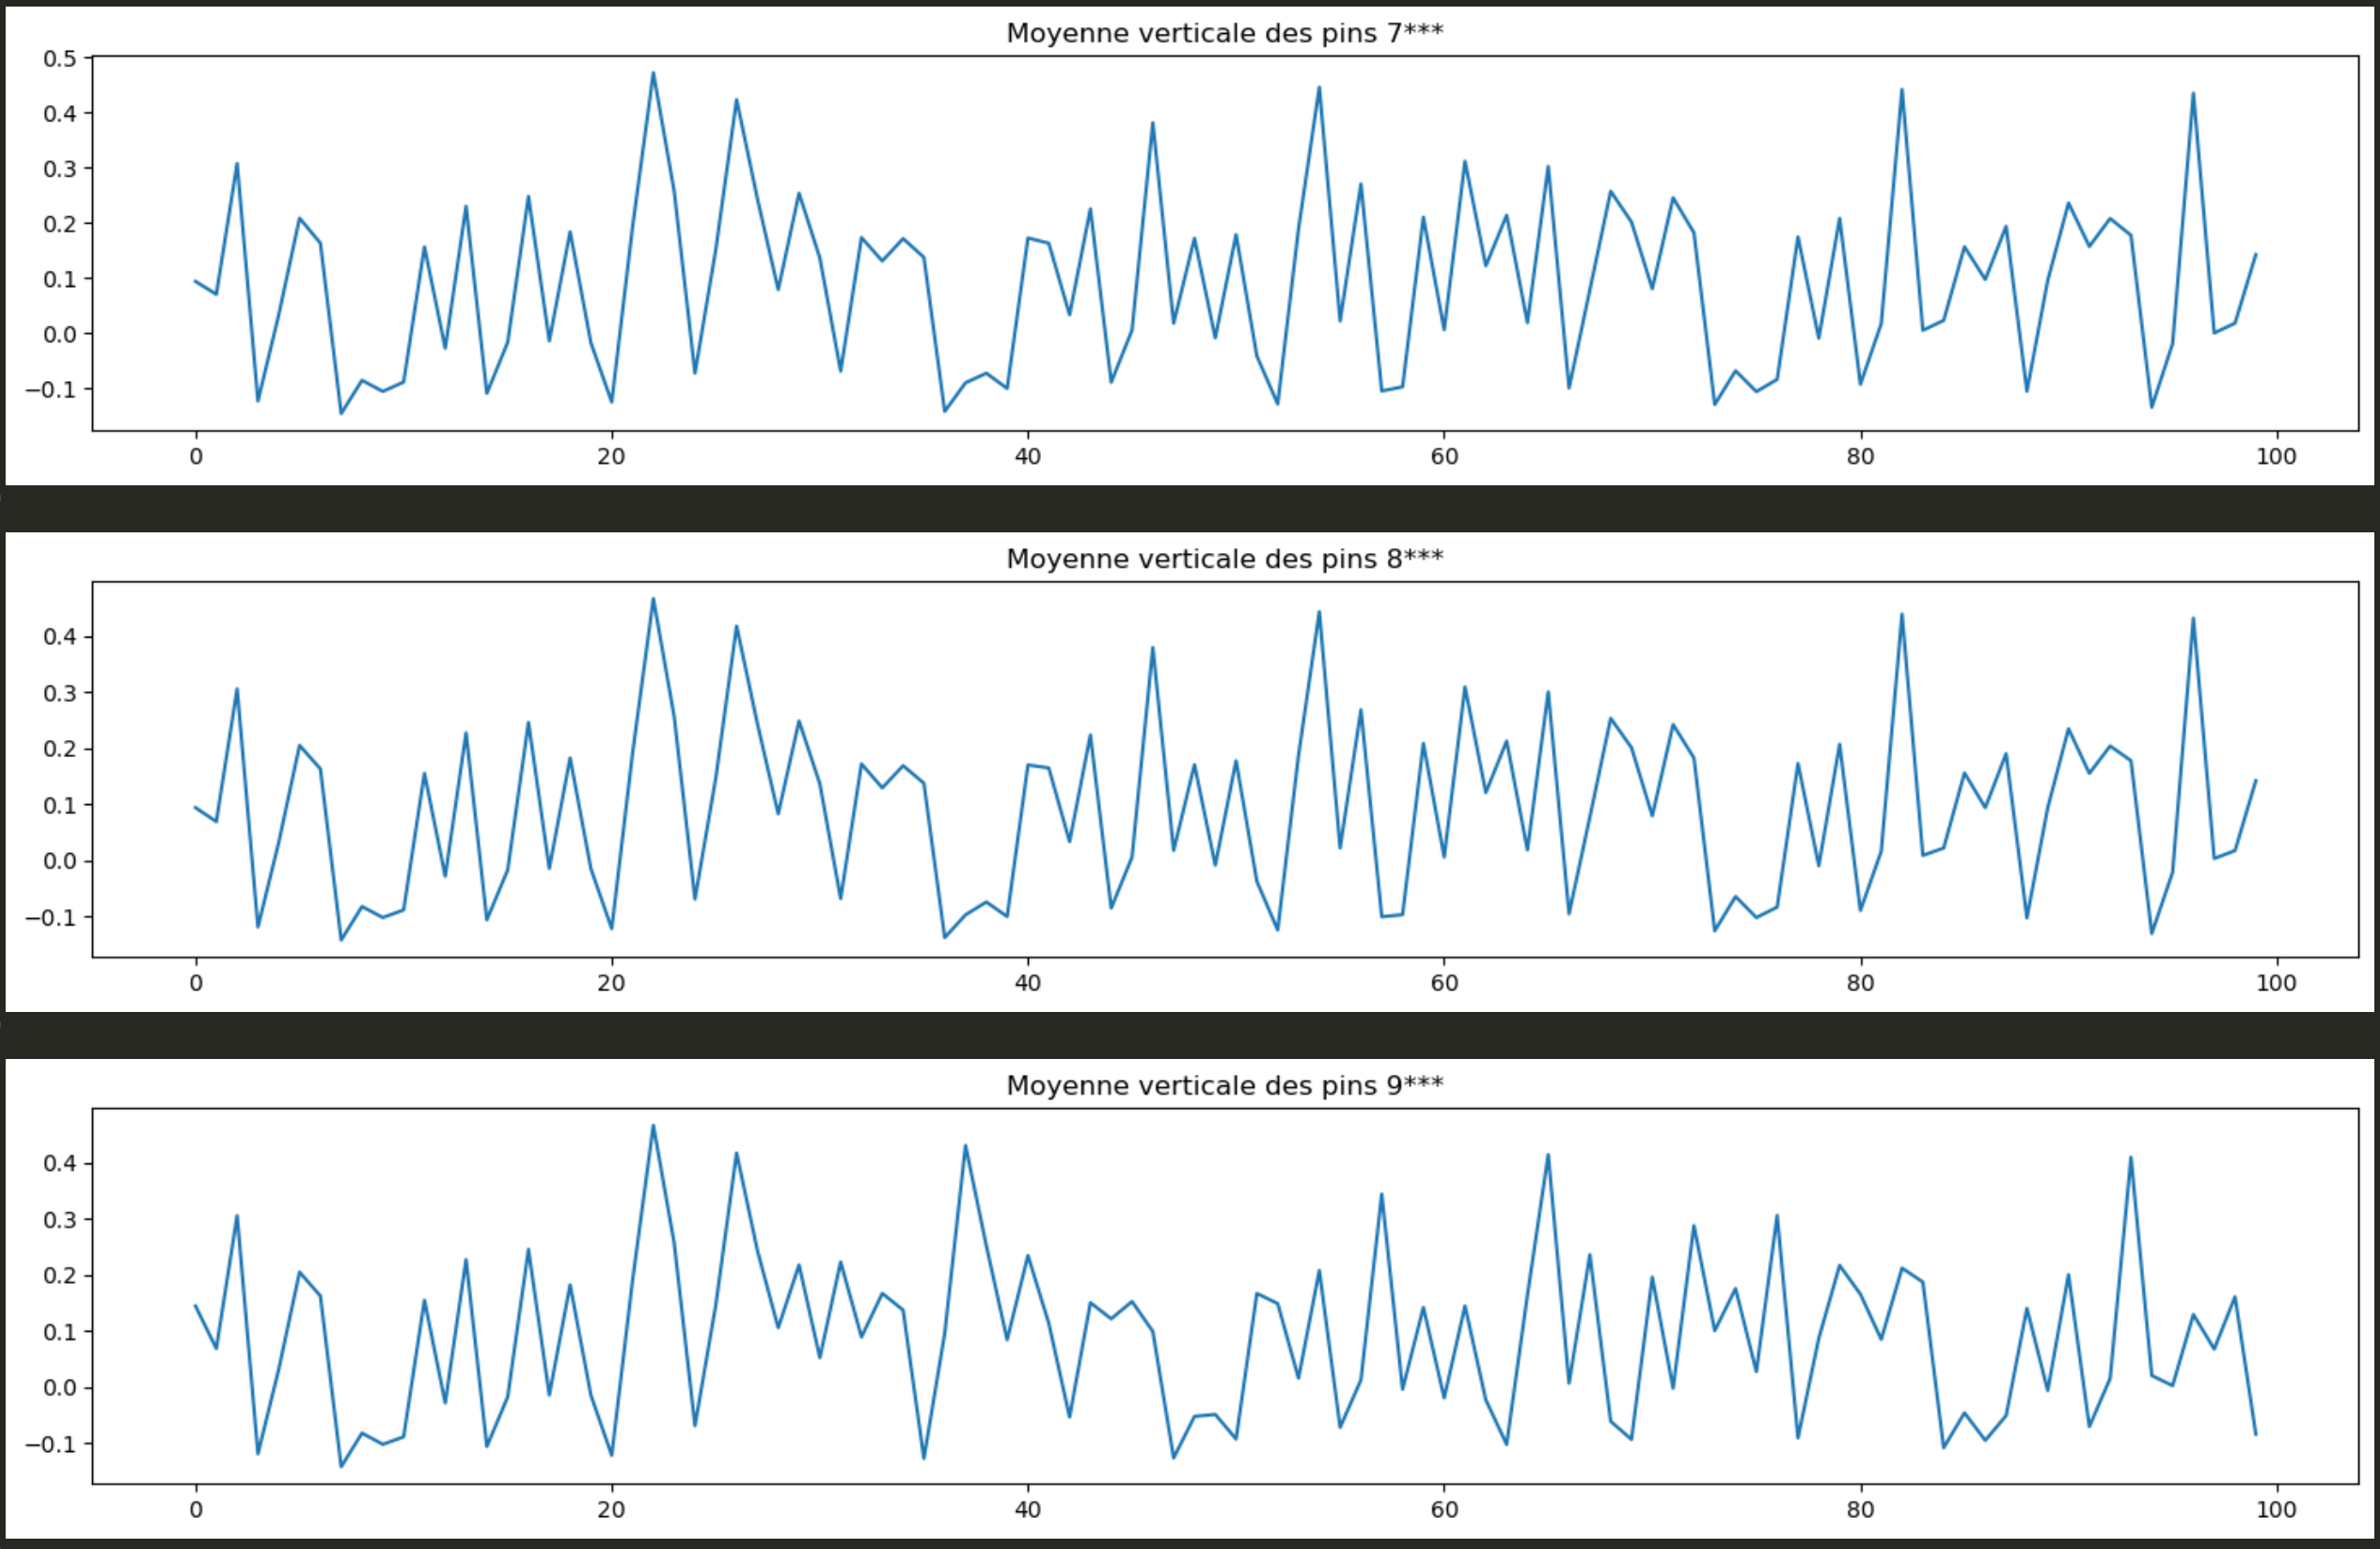
\includegraphics[width=0.7\textwidth]{img/sca/dfa/pin1.png}
    }
    \only<2>{
        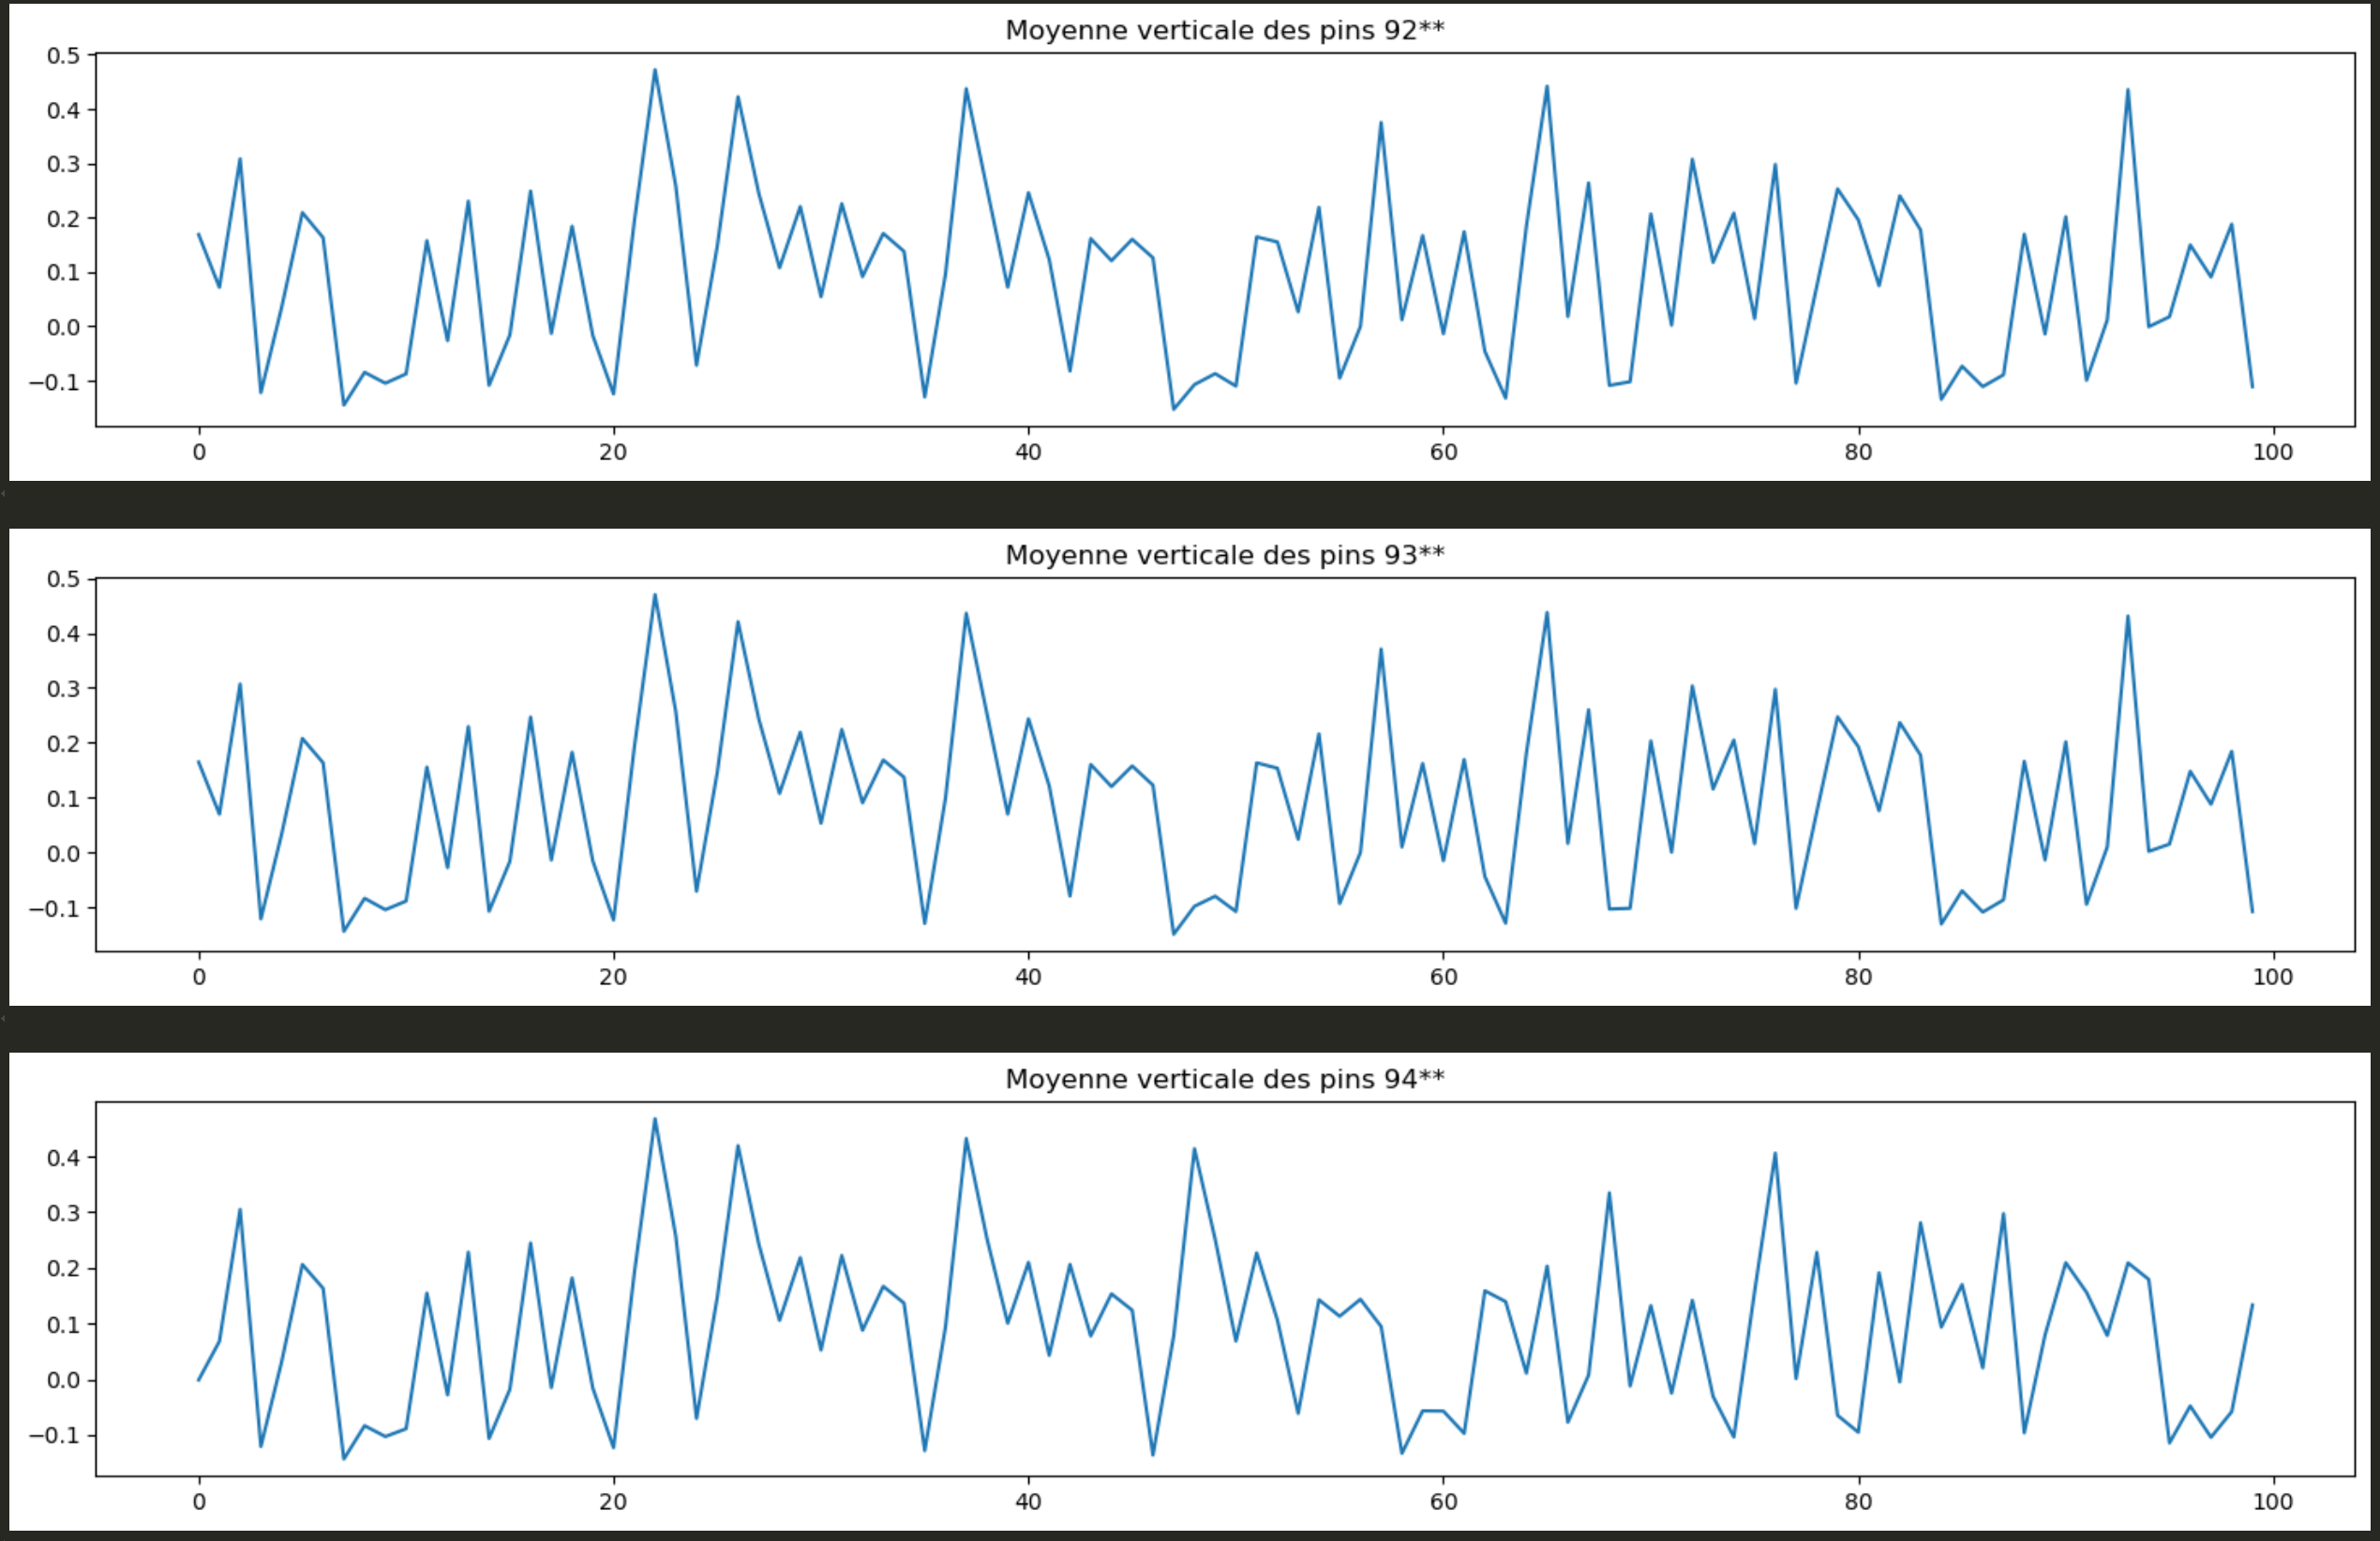
\includegraphics[width=0.7\textwidth]{img/sca/dfa/pin2.png}
    }
    \only<3>{
        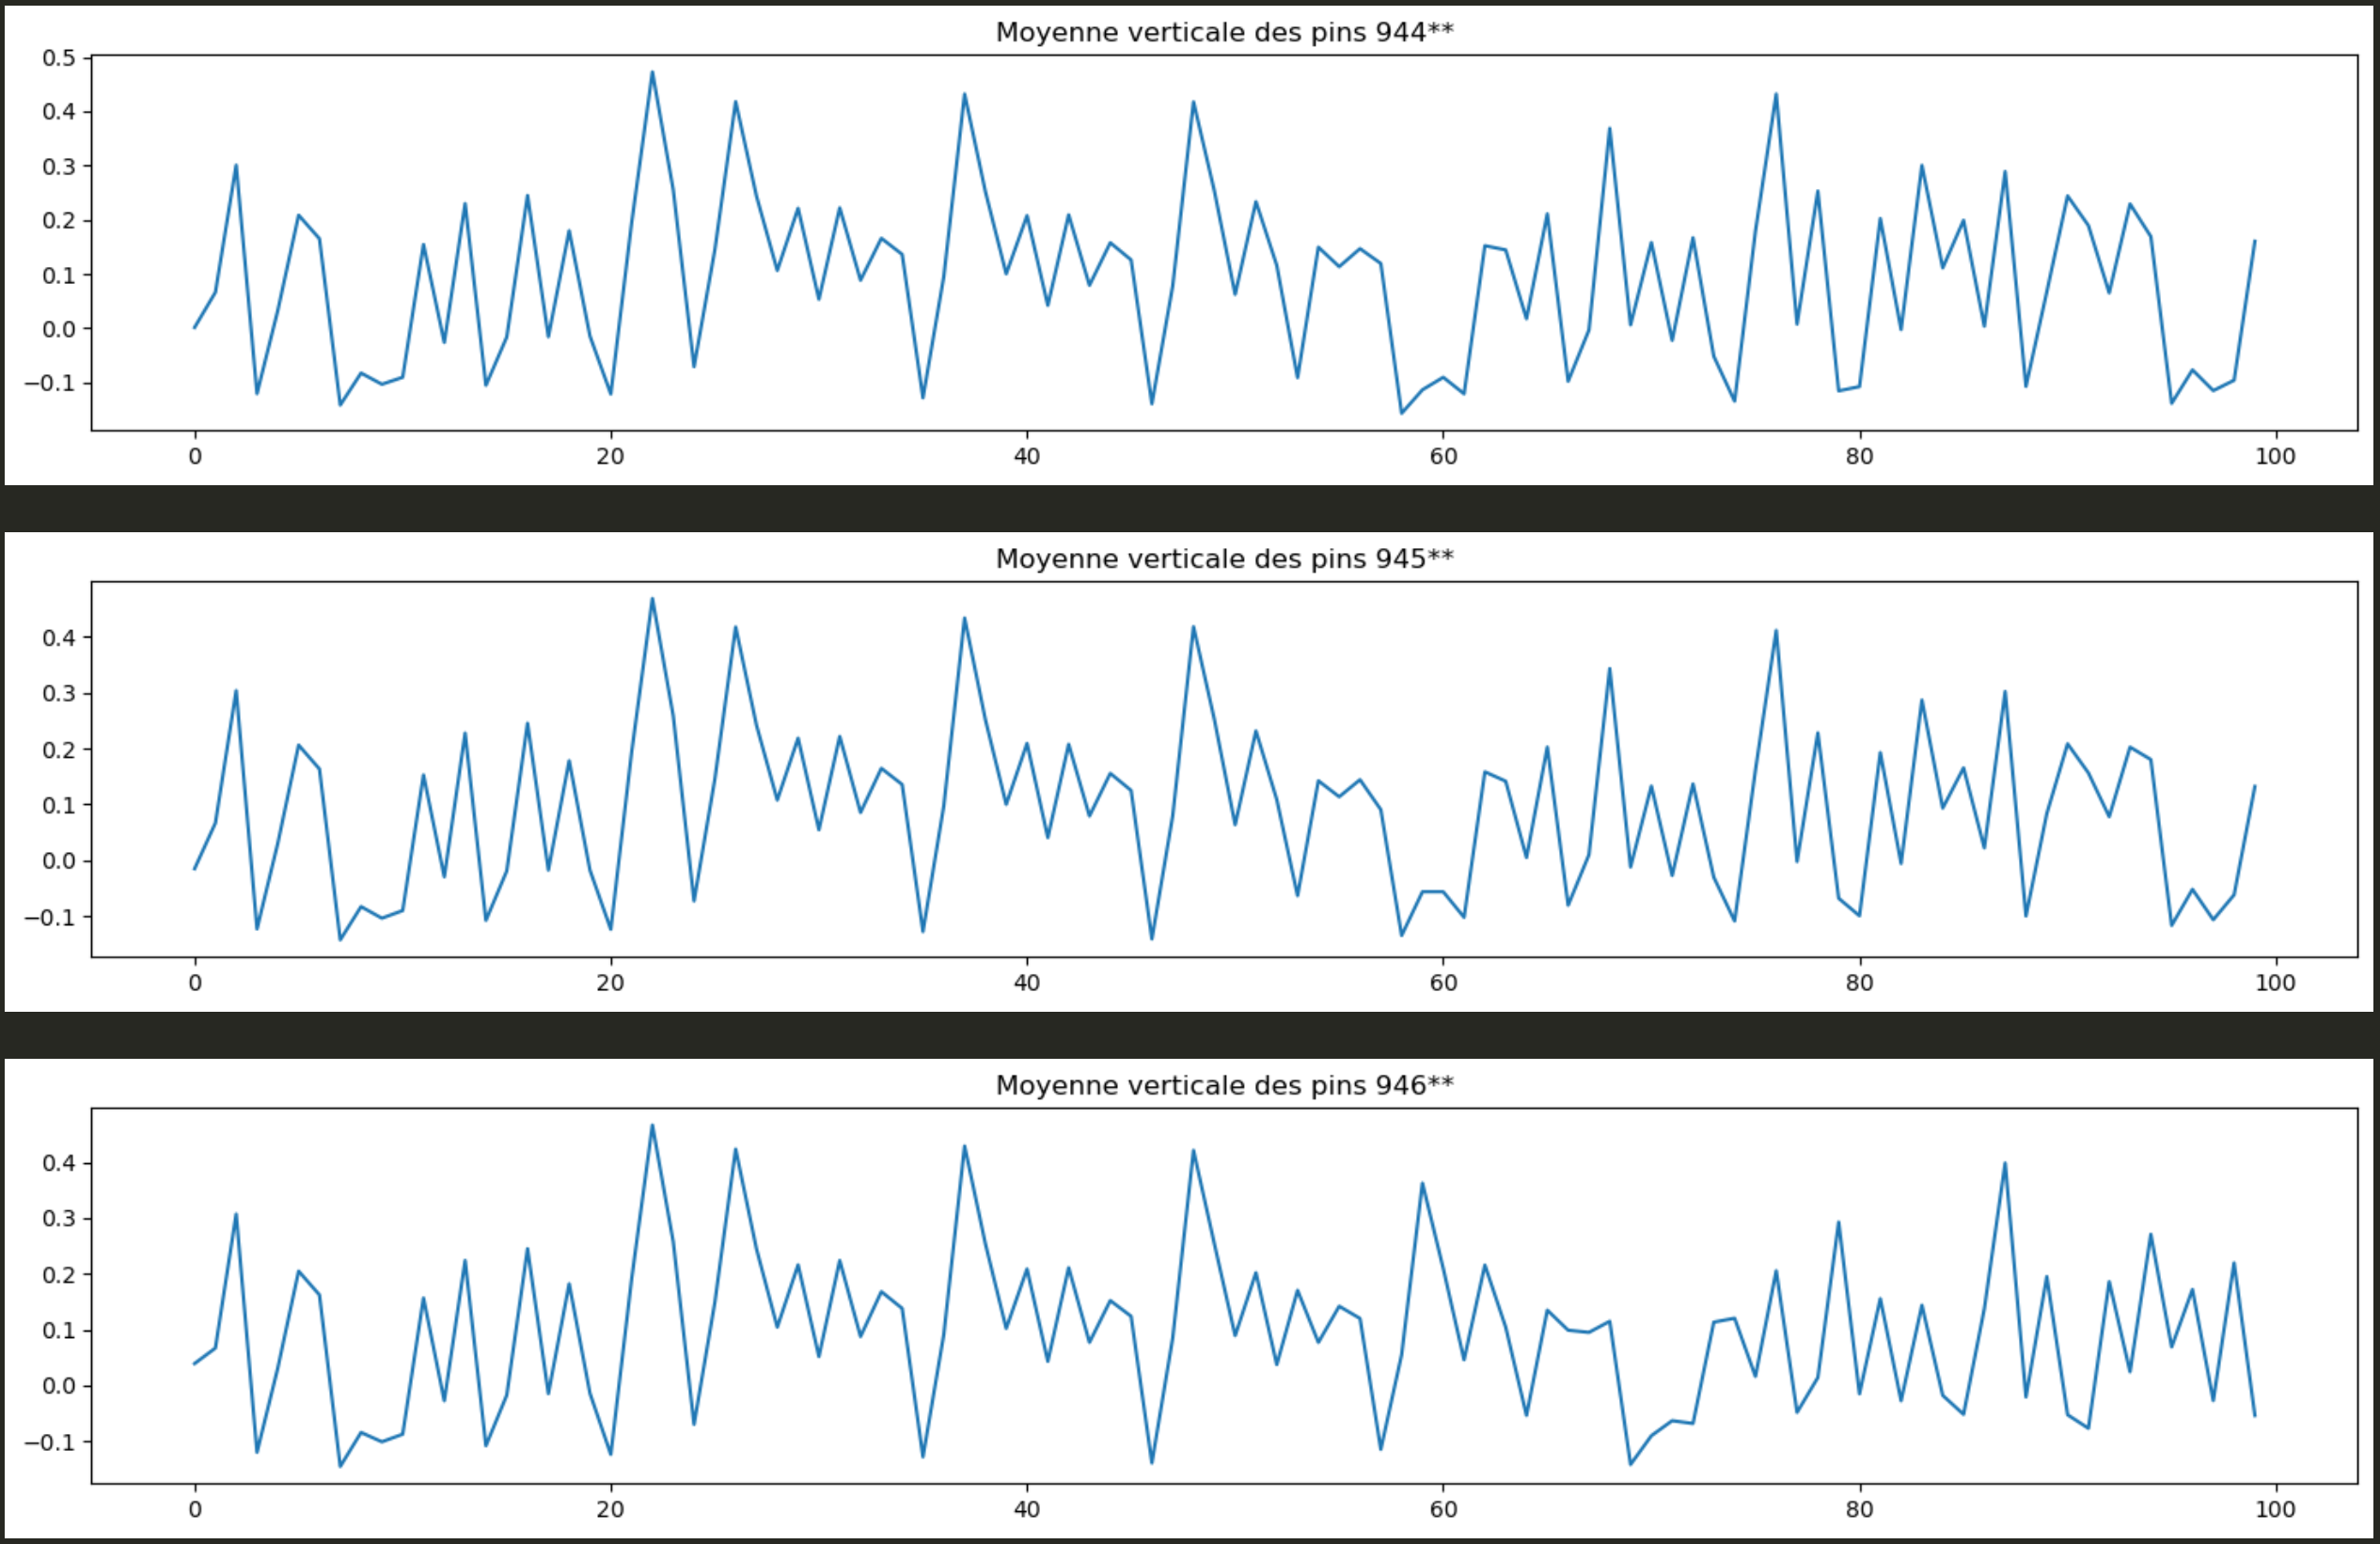
\includegraphics[width=0.7\textwidth]{img/sca/dfa/pin3.png}
    }
    \only<4->{
        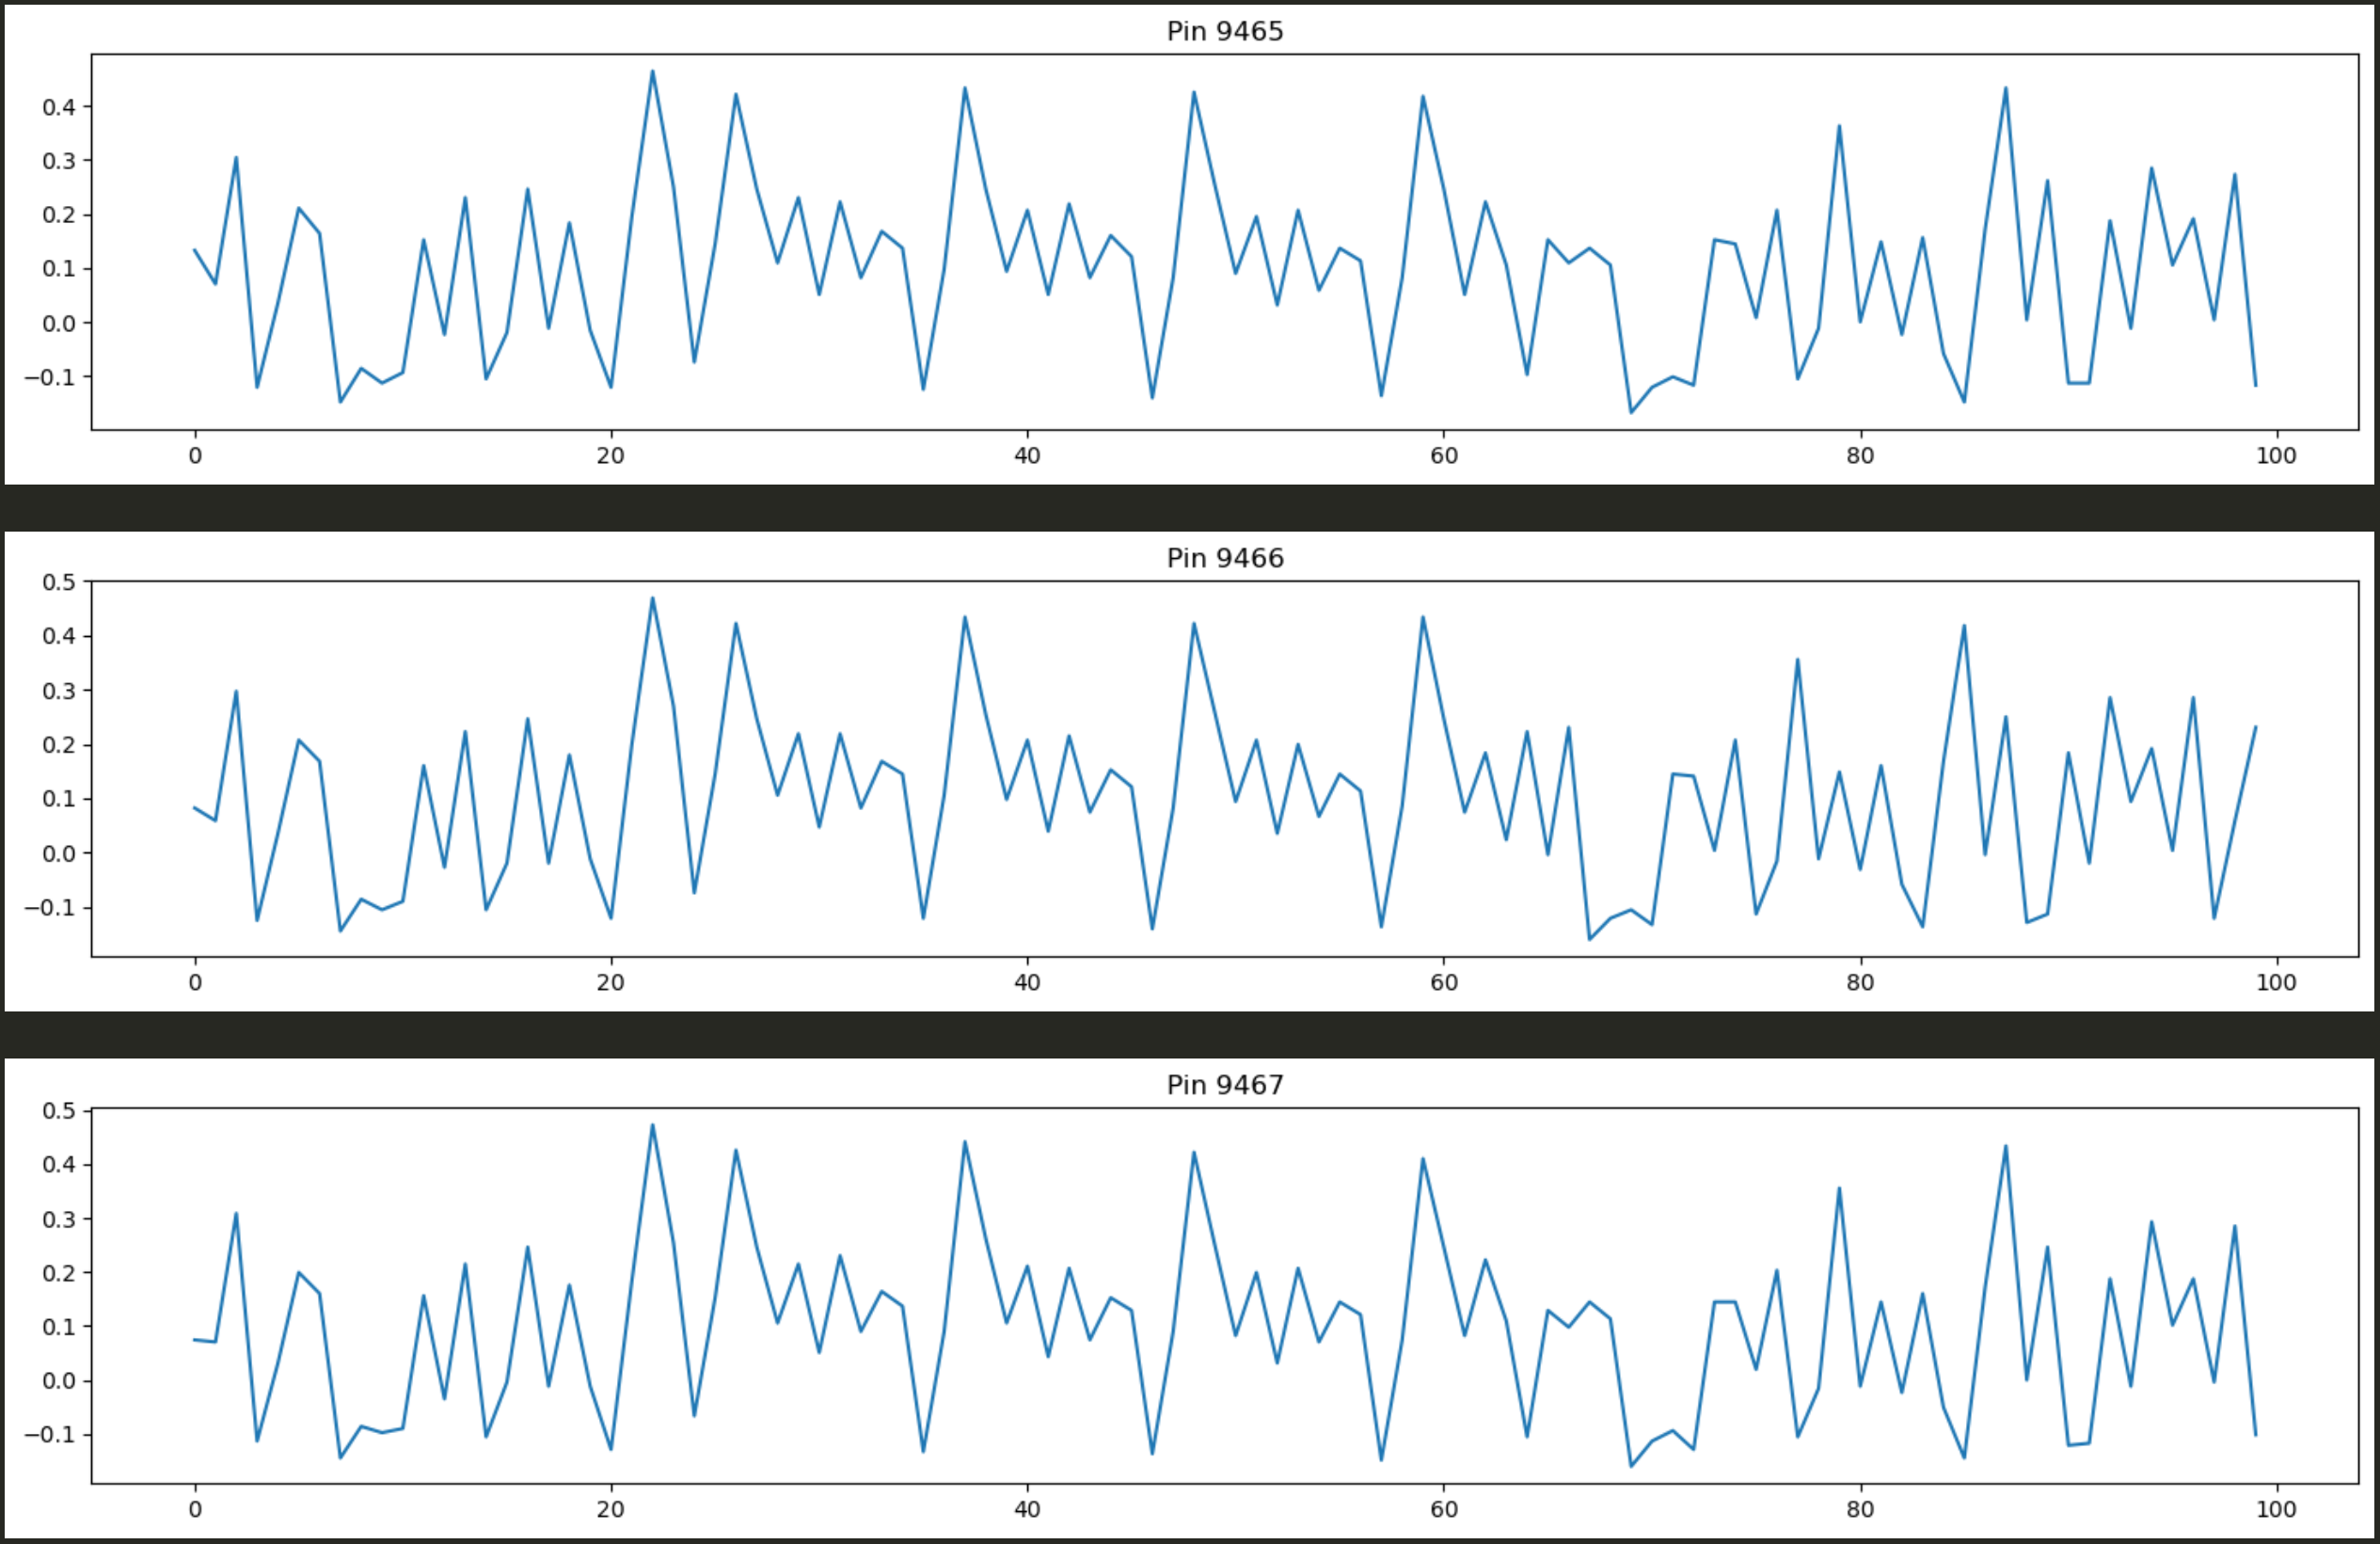
\includegraphics[width=0.7\textwidth]{img/sca/dfa/pin4.png}
    }
    \only<5>{\flag}
\end{frame}
\subsection{Attaques par fautes sur RSA et courbes elliptiques}
\begin{frame}{Attaques par faute sur RSA et ECDSA}
    \large{\centerline{\textbf{Bellcore et LLL}}}
\end{frame}

\begin{frame}{No Divide just Conquer \FiveStar/\FiveStar\FiveStar/\FiveStar\FiveStar\FiveStar \hfill 60/\textcolor{red}{21/6 résolutions}}
    \begin{columns}[c]
        \column{.50\textwidth}
        \begin{center}                  
            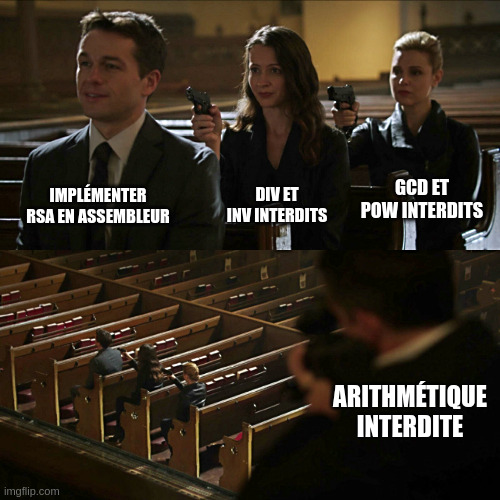
\includegraphics[width=0.9\textwidth]{img/meme/rsa-intro.png}
        \end{center}

        \column{.50\textwidth} % 
           \begin{outline}
               \1 Objectif
                \2 Implémenter RSA en assembleur-like
                \2 Avec de plus en plus de restrictions
           \end{outline}
    \end{columns}
\end{frame}

\begin{frame}{Atomic Secable \FiveStar\FiveStar\FiveStar \hfill \textcolor{red}{4 résolutions}}
\begin{columns}[c]
        \column{.50\textwidth}
        \begin{center}                  
            
\includegraphics[width=0.65\textwidth]{img/meme/atomic-secable-intro.png}
        \end{center}

        \column{.50\textwidth} %
           \begin{outline}
                \1 Objectif
                    \2 Récupérer la clef secrète ECDSA
                \pause
                \1 Données
                    \2 65 536 signatures fautées avec la clef
                \pause
                \1 Capacités d'attaquant
                    \2 Fauter aléatoirement une liste d'instruction donnée
           \end{outline}
    \end{columns}
\end{frame}

\begin{frame}{Attaque à information partielle sur ECDSA \footnote{\cite{demicheli:hal-03045663}}}

\[\left\{
\begin{array}{c c c}
\k{s_1} & = &\u{k_1}^{-1}\left(\k{h_1}+\k{r_1}*\u{d}\right) \mod \k{n} \\
\k{s_2} & = &\u{k_2}^{-1}\left(\k{h_2}+\k{r_2}*\u{d}\right) \mod \k{n} \\
&\vdots& \\
\k{s_m} & = &\u{k_m}^{-1}\left(\k{h_m}+\k{r_m}*\u{d}\right) \mod \k{n} \\
\end{array}
\right.
\pause
\;\Rightarrow\;
\left\{
\begin{array}{c c c}
\u{k_1}+\k{t_1}\u{k_m} + \k{u_1} & = & 0 \mod \k{n} \\
\u{k_2}+\k{t_2}\u{k_m} + \k{u_2} & = & 0 \mod \k{n} \\
&\vdots&\\
\u{k_{m-1}}+\k{t_{m-1}}\u{k_m} + \k{u_{m-1}} & = & 0 \mod \k{n} \\
\end{array}
\right.\]

\pause
\begin{center}
    On espère que les $\u{k_i}$ soient suffisamment petits (connaître les bits de poids fort)
    \pause
    
    Le réseau suivant contient le vecteur $(\u{k_1},\;\dots,\;\u{k_m},\;\k{K})$
\end{center}
    \begin{columns}[c]
        \column{.35\textwidth}
        \[\left(
        \begin{array}{c c c c c c}
        \k{n} &   &        &   &   &    \\
          & \k{n} &        &   &   &   \\
          &   & \ddots &   &   &    \\
          &   &        & \k{n} &   &   \\
        \k{t_1}  &   \k{t_2} &  \dots    &  \k{t_{m-1}}  & 1 &   \\
        \k{u_1}  &   \k{u_2} &  \dots    &  \k{u_{m-1}}  & 0 & K  \\
        \end{array}
        \right)\]
        \pause
        \column{.65\textwidth} % 
           \begin{outline}
           \1 Tricks sur l'algorithme LLL
            \pause
            \2 La diagonale de $\k{n}$ permet de simuler un réseau modulaire
            \pause
            \2 K est choisi grand pour forcer la dernière ligne à 1
           \end{outline}
    \end{columns}


\end{frame}


\begin{frame}{Dans le cadre du challenge}
    \begin{columns}[c]
\column{.55\textwidth}
        \begin{outline}
            \1Retrouver la clef privée: si un des $\u{k_i}$ \textbf{ou certains bits de plusieurs $\u{k_i}$} sont connus, c'est gagné
            
            \uncover<2->{
            \1 Objectif : distinguer les deux cas
            }
                \uncover<3->{ 
                \2 Par SCA (opérations différentes)
                }
                \uncover<4->{
                \2 Par timing (premières opérations ignorées)
                    \3 Temps d’exécution non constant
                }
                \uncover<5->{
                \2 Un seul des deux cas resiste à une faute
                    \3 On faute les 16 premières opérations
                    \3 Les survivants commencent par 16 zéros
                }
        \end{outline}
\column{.45\textwidth} % 
    \uncover<2->{
      \begin{algorithm}[H]
        \SetAlgoLined
        \KwIn{Scalaire $k = (k_{n-1}, \dots, k_0)_2$, Point $P$}
        \KwOut{$Q = [k]P$}
        $(R_0,R_1) \leftarrow (\mathcal{O},P)$\;
        \For{$i \leftarrow n-1$ \KwTo $0$}{
            \If{$k_i = 0$}{
                $(R_0, R_1) \leftarrow ([2]R_0,R_0 + R_1)$\;
            }
            \Else{
                $(R_0,R_1) \leftarrow (R_0 + R_1,[2]R_1)$\;
            }
        }
        \Return $R_0$\;
        \caption{Echelle de Montgomery}
    \end{algorithm}
    }
    \end{columns}

\end{frame}


\subsection{Fuites de l'état interne AES}
\begin{frame}{Fuite de l'état interne AES}
    \large{\centerline{\textbf{Dévoiler la clef, un tour à la fois}}}
\end{frame}

\begin{frame}{AES Distrace \FiveStar\FiveStar \hfill 10 résolutions}
    \begin{columns}[c]
        \column{.45\textwidth}
        \begin{center}                  
            
\includegraphics[width=0.8\textwidth]{img/meme/distrace-intro.png}
        \end{center}

        \column{.65\textwidth} % 
           \begin{outline}
               \1 Objectif
                \2 Décoder un message chiffré avec AES

            \pause
               \1 Données
                \2 Observer l'évolution d'un registre à chaque étape du chiffrement 
           \end{outline}
    \end{columns}
\end{frame}


\begin{frame}[fragile]
\frametitle{Capacité d'attaquant}

\begin{center}
    Révéler une variable (registre) à une ligne  (IP) donnée
\end{center}

    \begin{columns}[c]
        \column{.50\textwidth}
   % \begin{columns}[c]
    %    \column{.45\textwidth}

\begin{small}
\renewcommand{\lstlistingname}{}

\begin{lstlisting}[language=C,numbers=left, numberstyle=\tiny, numbersep=5pt, xleftmargin=0pt]
for (int i = 0; i < 16; i++){
    s[i] = s[i] ^ k[i];
}
\end{lstlisting}

\vspace{1cm}

\onslide<3->
\begin{lstlisting}[language=C,,,numbers=left, numberstyle=\tiny, numbersep=5pt, xleftmargin=0pt]
    s[0] = s[0] ^ k[0];
    s[1] = s[1] ^ k[1];
    ...
    s[14] = s[14] ^ k[14];
    s[15] = s[15] ^ k[15];

\end{lstlisting}

\end{small}

        \column{.50\textwidth} % 
           \begin{outline}
            \onslide<1->
                \1 \textbf{"Donne moi $k$ à la ligne 2"}
                    \2 On récupère tout $k$

                \vspace{0.45cm}
                \pause
                
                \1 Loop-unrolling
                    \2 Réduit l'overhead lié aux boucles
                    \2 Binaires plus lourd

                \vspace{0.5cm}
                \pause
                
                \1 \textbf{"Donne moi $k$ à la ligne 2"}
                    \2 On récupère un byte de $k$
            \end{outline}
            \vspace{0.6cm}
            
    \end{columns}

\end{frame}


\begin{frame}{Analyse du loop-unrolling (code C)}
    \begin{itemize}
        \item \textbf{KeySchedule} : 1 bytes du keySchedule par tour  (sauf un) \hfill 48 bits de bruteforce 
        
        \pause
        
        \item \textbf{MixColumns} : 1 byte de l'état interne par tour
        \item \textbf{AddRoundKey} : 1 byte de l'état interne/clef par tour \hfill  40 bits de bruteforce

        \pause
        
        \item \textbf{Shiftrows + Subbytes} : 4 bytes (une colonne) de l'état interne par tour
    \end{itemize}
    
    \pause

    \center
    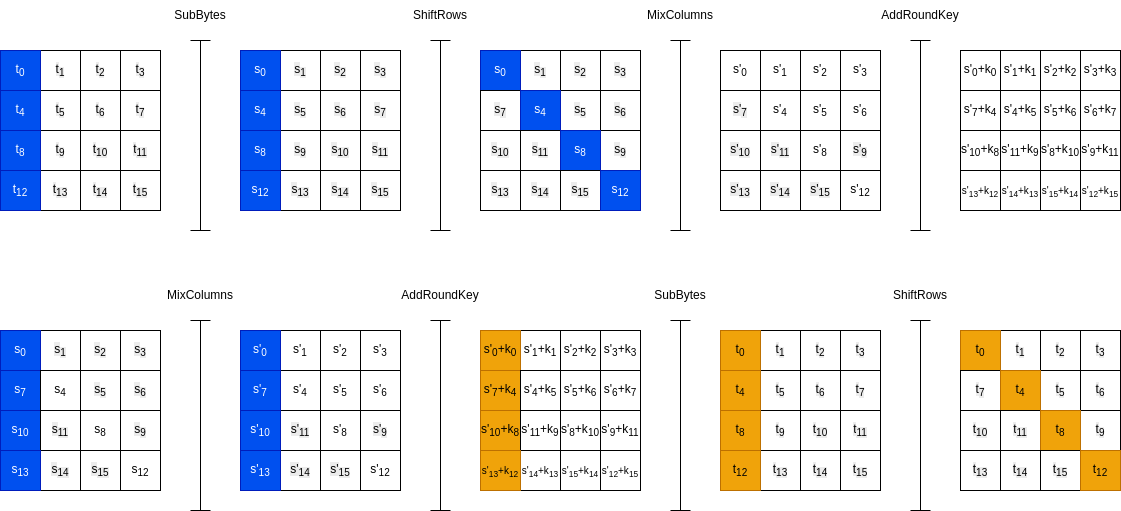
\includegraphics[width=0.75\textwidth]{img/sca/aes-distrace/attack_sbsr.png}

\end{frame}

\begin{frame}{Rappel sur le KeySchedule}
    \centering
    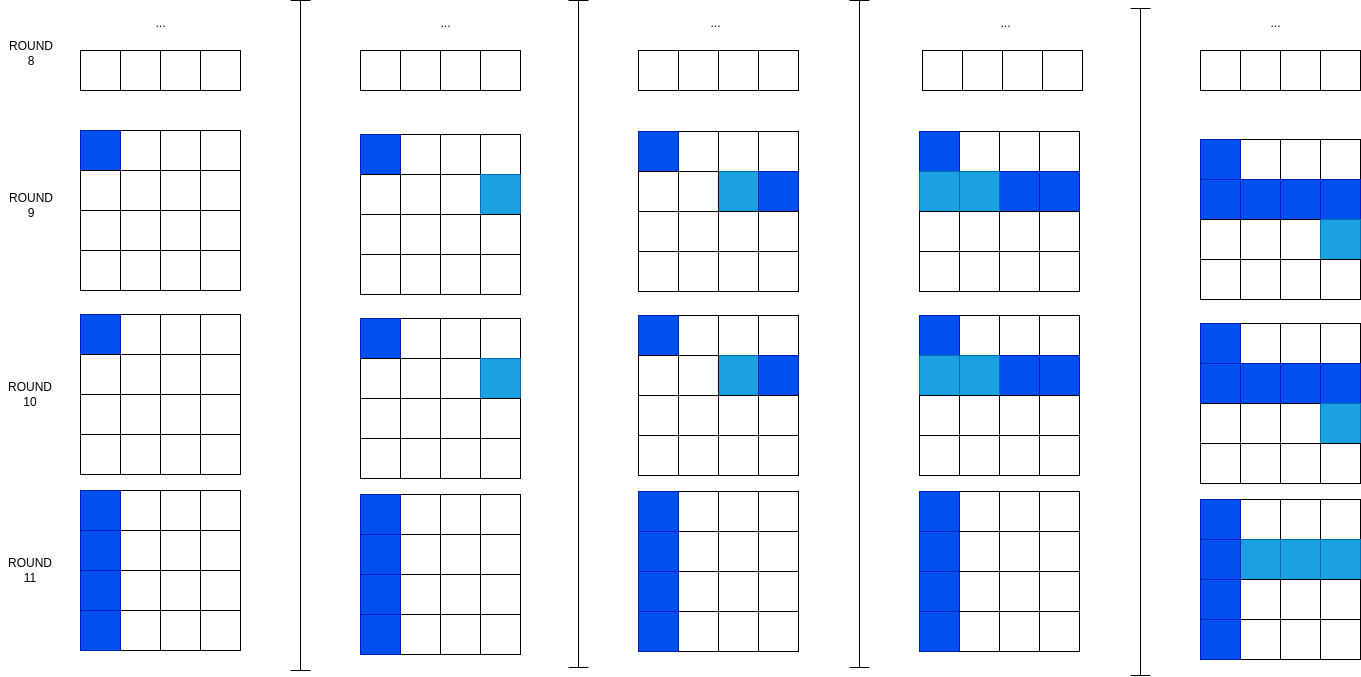
\includegraphics[width=0.23\textwidth,clip,trim=0 0 1070 0]{img/sca/aes-distrace/full_recovery.png}
    \pause
    \hspace{0.5cm}
    \raisebox{0.4cm}{\rule{0.4pt}{7cm}}
    \hspace{0.4cm}
    \hspace{0.5cm}
    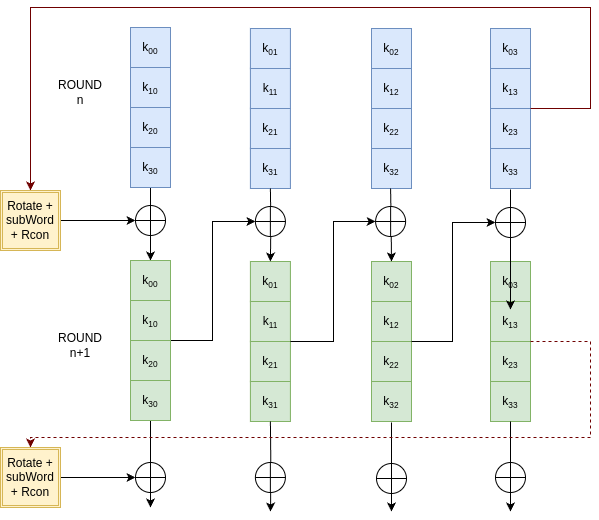
\includegraphics[width=0.6\textwidth]{img/sca/aes-distrace/keysched.png}
\end{frame}

\begin{frame}{Propagation de connaissance}
    \begin{columns}[T,onlytextwidth]
      \column{0.45\textwidth}
      \vspace{1cm}
        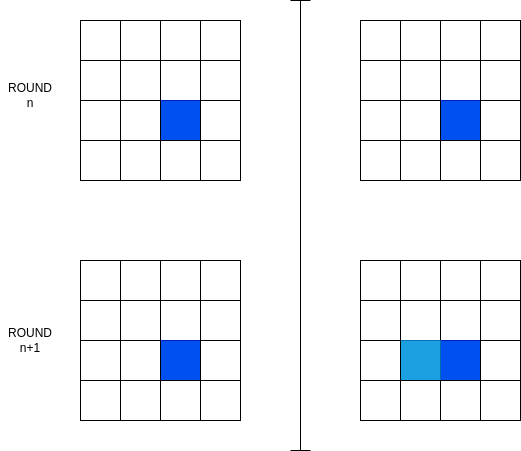
\includegraphics[width=\linewidth]{img/sca/aes-distrace/ex1.png}\\[1ex]
        \pause
      \column{0.45\textwidth}
        \vspace{1cm}
        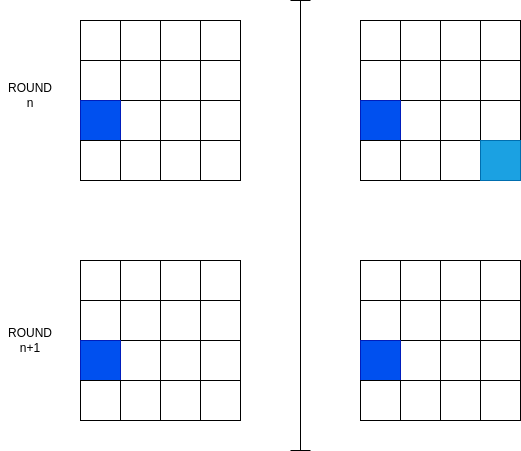
\includegraphics[width=\linewidth]{img/sca/aes-distrace/ex4.png}
    \end{columns}
\end{frame}


\begin{frame}{Full recovery}
    \begin{center}
        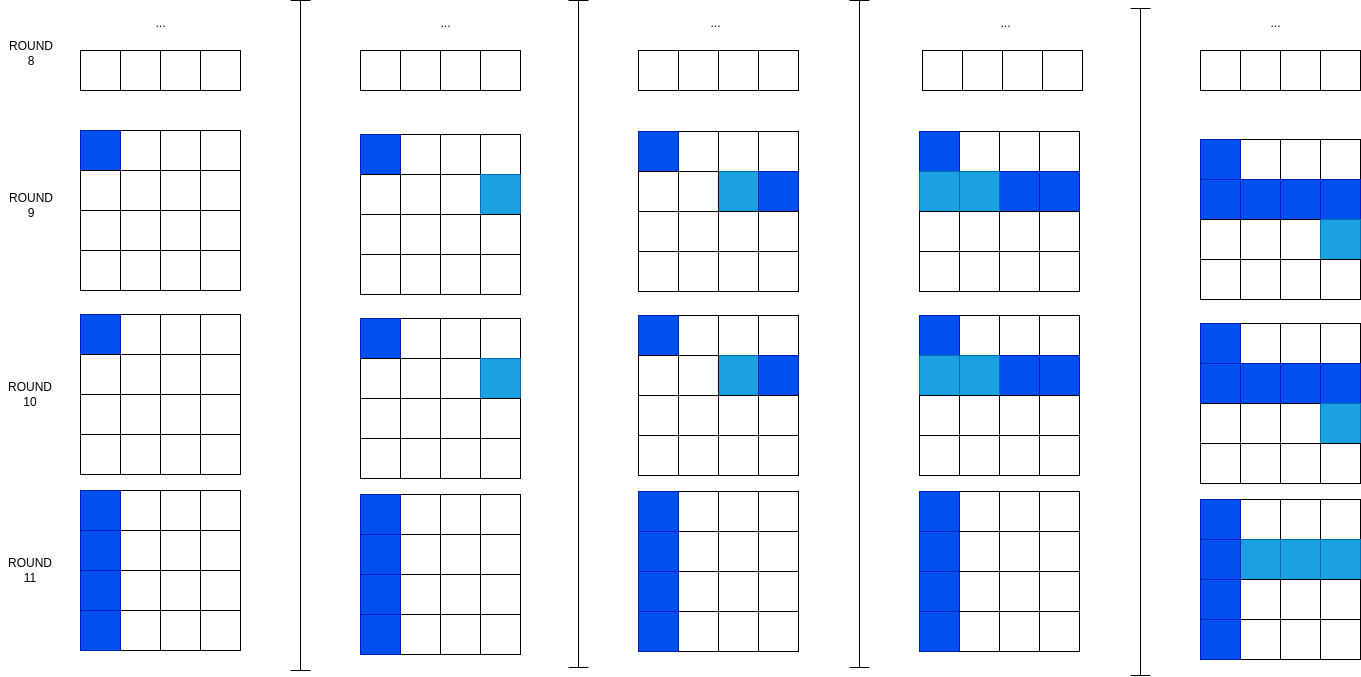
\includegraphics[width=0.85\textwidth]{img/sca/aes-distrace/full_recovery.png}
    \end{center}
    \pause
    
    Au final, il reste 3 bytes à bruteforcer (24 bits) \flag
\end{frame}



\section{Cryptographie}
\subsection{Introduction : les classiques de ctf}
\begin{frame}{Introduction : Les classiques de ctf}
    \large{\centerline{\textbf{Cinq challenges de démarrage}}}

\end{frame}

%------------------------------------------------
%------------------------------------------------

\begin{frame}{RSA-WTF \FiveStar (speedrun)\hfill 202 résolutions}
    \begin{columns}[c]
        \column{.45\textwidth}
        \begin{center}                  
            
\includegraphics[width=0.8\textwidth]{img/meme/rsa-wtf-intro.png}
        \end{center}

        \column{.65\textwidth} % 
           \begin{outline}
               \1 Objectif
                \2 Récupérer \u{$d$} aléatoire sur 666 bits

            \pause
               \1 Données
                \2 $\k{d_p} = \u{d}^{-1} \mod (\k{p}-1)$
                \2 $\k{d_q} = \u{d}^{-1} \mod (\k{q}-1)$

                \pause
                
                \2 $\k{p, q}$ sur 512 bits

            \pause
               \1 Solution
                \2 Théorème des restes chinois pour avoir
                    \[d \mod lcm(p-1,q-1) \]
            
            \pause
               \1 First Blood en 65 secondes \flag{}
           \end{outline}
    \end{columns}
\end{frame}

%------------------------------------------------
%------------------------------------------------

\begin{frame}{CocoRiCo \FiveStar \hfill 366 résolutions}
    \begin{columns}[c]
        \column{.45\textwidth}
        \begin{center}                  
            
\includegraphics[width=0.8\textwidth]{img/meme/cocorico.png}
        \end{center}

        \column{.65\textwidth} % 
           \begin{outline}
               \1 Objectif
                \2 Forger un chiffrement + authentification
               \1 Données
                \2 Accès à un oracle
               \1 Solution
                \2 Malléabilité d'AES-CTR / AES-OFB
               \1 First Blood en 7 minutes \flag{}
           \end{outline}
    \end{columns}
\end{frame}

%------------------------------------------------
%------------------------------------------------

\begin{frame}{Problèmeuh \FiveStar \FiveStar \hfill 156 résolutions}
    \begin{columns}[c]
        \column{.45\textwidth}
        \begin{center}                  
            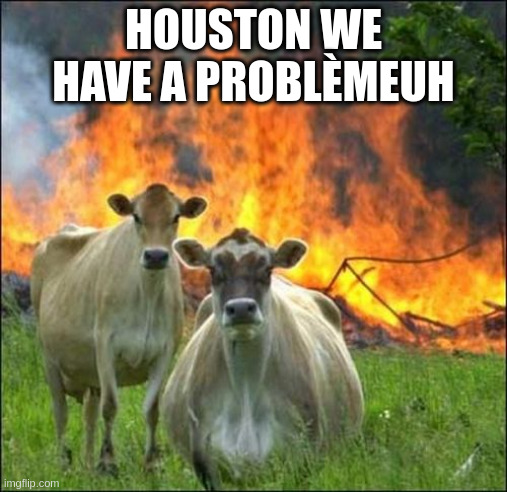
\includegraphics[width=0.8\textwidth]{img/meme/problemeuh-intro.png}
        \end{center}

        \column{.65\textwidth} % 
           \begin{outline}
               \1 Objectif
                \2 Résoudre un système d'équation diophantienne
                \[\left\{
                    \begin{array}{r c l}
                        \u{a} &=&  487 \u{c} \\
                        59\u{a} &=& 485 \u{b} \\
                        \u{x} ^ 2 &=& \u{a} + \u{b} \\
                        \u{y} (3 \u{y} - 1) &=& 2 \u{b} \\
                    \end{array}
                \right.\]
               \1 Solution
                \2 Se ramener à l'équation de Pell :
                 \[(6\u{y} - 1)^2 - 145710941544 \u{k}^2 = 1\]
               \1 Peut se résoudre avec des fractions continues
               \1 \url{https://www.alpertron.com.ar/METHODS.HTM} \flag{}
           \end{outline}
    \end{columns}
\end{frame}

%------------------------------------------------
%------------------------------------------------

\begin{frame}{La quête de l'anneau \FiveStar \hfill 585 résolutions}
    \begin{columns}[c]
        \column{.45\textwidth}
        \begin{center}                  
            
\includegraphics[width=0.8\textwidth]{img/meme/la-quete-intro.png}
        \end{center}

        \column{.65\textwidth} % 
           \begin{outline}
               \1 Objectif
                \2 Résoudre des équations modulo $\u{s}$ aléatoire 
                \2 $E : \u{m} \mapsto \k{IV}\cdot \u{m} \mod \u{s} = \k{c}$
                \2 $E^{-1} : \k{c} \mapsto \u{IV^{-1}}\cdot \k{c} \mod \u{s} = \u{m}$

                \vspace{0.3cm}
                \pause
                
               \1 Données
                \2 Deux clairs connu $E(\k{m_1}) = \k{c_1}$ et $E(\k{m_2}) = \k{c_2}$
                \2 Un message à déchiffrer $\u{m_3}$ sachant $\k{c_3}$
               
                \vspace{0.3cm}
                \pause 
                
               \1 Solution
                \2 $\left\{ \begin{array}{r c l} \k{c_1} &=& \k{IV_1}\cdot\k{m_1}+\u{k_1}\u{s} \\
                        \k{c_2} &=& \k{IV_2}\cdot\k{m_2} +\u{k_2}\u{s} \\
                    \end{array}
                \right.$

                
                \pause
                \2 $s = PGCD(\k{c_1}-\k{IV_1}\cdot\k{m_1},\k{c_2}-\k{IV_2}\cdot\k{m_2})$ \flag{}
           \end{outline}
    \end{columns}
\end{frame}


%------------------------------------------------
%------------------------------------------------

\begin{frame}{La revanche de Sauron \FiveStar \FiveStar (speedrun) \hfill 9 résolutions}
    \begin{columns}[c]
        \column{.45\textwidth}
        \begin{center}                  
            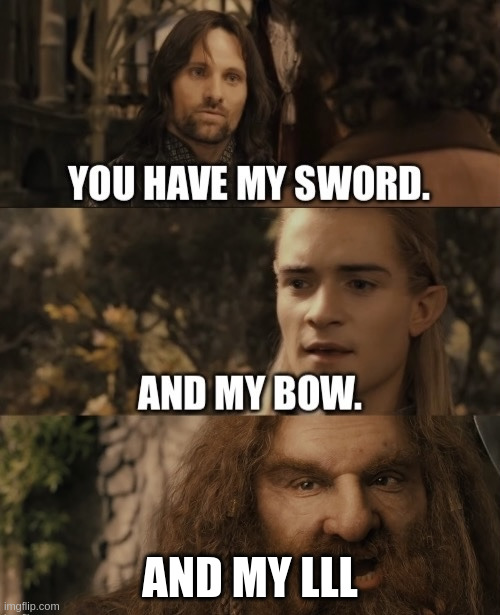
\includegraphics[width=0.8\textwidth]{img/meme/la-revanche-intro.png}
        \end{center}

        \column{.65\textwidth} % 
           \begin{outline}
            \1 Objectif
                \2 Résoudre des équations modulo $\u{s}$ aléatoire 
                \2 $E : \u{m} \mapsto \k{IV}\cdot \u{m} \mod \u{s} = \k{c}$
                \2 $E^{-1} : \k{c} \mapsto \u{IV^{-1}}\cdot \k{c} \mod \u{s} = \u{m}$

               \1 Données
                \2 Les chiffrés : $E(\u{m_1})=\k{c_1}$ et $E(\u{m_2}) = \k{c_2}$

                \pause
                
               \1 Solution
                \2  $\left\{ \begin{array}{r c l} \k{c_1} &=& \k{IV_1}\cdot\u{m_1}+\u{k_1}\u{s} \\
                        \k{c_2} &=& \k{IV_2}\cdot\u{m_2} +\u{k_2}\u{s} \\
                    \end{array}
                \right.$
                
                \vspace{0.3cm}
                
                \2 $\k{c_1}\u{k_2} - \k{IV_1}\u{m_1}\u{k_2} - \k{c_2}\u{k_1} +  \k{IV_2}\u{m_2}\u{k_1} =  0$

                \pause
                \vspace{0.3cm}

                \pause 
                
                \2 $\u{s}$ et $\k{IV_i}$ font 1024 bits, $\u{m_i}$ font $256$ bits
            \1 Résoudre avec Coppersmith ou LLL ?
           \end{outline}
    \end{columns}
\end{frame}

%------------------------------------------------
%------------------------------------------------

\begin{frame}{Coppersmith / LLL}
\begin{block}{Utilisation de l'algorithme LLL en ctf}
    Trouve des combinaisons linéaires anormalement petites de vecteurs.
\end{block}

\pause

\vspace{-0.4cm}

     \[
        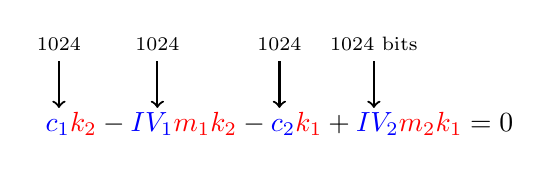
\begin{tikzpicture}[baseline=(eq.base)]
            \node (eq) at (0,0) {$\k{c_1}\u{k_2} - \k{IV_1}\u{m_1}\u{k_2} - \k{c_2}\u{k_1} +  \k{IV_2}\u{m_2}\u{k_1} =  0$};

            \foreach \x/\label in {
                -2.8/1024,
                -1.55/1024,
                 0./1024,
                 1.2/1024 bits
            } {
                \draw[<-, thick] (\x,0.2) -- ++(0,0.6) node[above] {\scriptsize \label};
            }
        \end{tikzpicture}
    \]

\pause

\begin{outline}
    \1 $0$ est engendré par $(\k{c_1})$, $(\k{IV_1})$, $(\k{c_2})$, $(\k{IV_2})$ 
        \pause
        \2[$\longrightarrow$]  LLL retourne bien $0$
    \1 Comment retrouver les coefficients utilisés?
    \pause
    \1 $\left[
    \begin{array}{ r c c c c}
        \k{c_1},  &1, &0, &0, &0  \\
        -\k{IV_1},&0, &1, &0, &0 \\
        -\k{c_2}, &0, &0, &1, &0 \\
        \k{IV_2}, &0, &0, &0, &1 \\
    \end{array}
    \right]$ engendre le vecteur $(0, \u{k_2},\u{m_1}\u{k_2},\u{k_1},\u{m_2}\u{k_1})$
    \pause
    \1 Il a pour taille (1, 256, 512, 256,512) bits. Est-il anormalement petit?
    \pause 
     \2[$\longrightarrow$] LLL trouve un vecteur de $(254, 251, 256, 255, 257)$ bits
\end{outline}
\end{frame} 

%------------------------------------------------
%------------------------------------------------



\begin{frame}{Changer la géométrie d'un réseau}

\begin{outline}
    \1 $\left[
    \begin{array}{r c c c c}
        \k{c_1} \times \mathbf{B},  &1, &0, &0, &0  \\
        -\k{IV_1} \times \mathbf{B}, &0, &1, &0, &0 \\
        -\k{c_2} \times \mathbf{B}, &0, &0, &1, &0 \\
        \k{IV_2} \times \mathbf{B}, &0, &0, &0, &1 \\
    \end{array}
    \right]$ engendre toujours $(0, \u{k_2},\u{m_1}\u{k_2},\u{k_1},\u{m_2}\u{k_1})$
    
    \pause \1 Un B gigantesque forcera la première composante à 0
        \2[$\longrightarrow$] LLL trouve un vecteur de taille $(1, 339, 339, 340, 341)$ bits
    \pause
    
    \vspace{0.5cm}
    
     \1 $\left[
    \begin{array}{r c c c c}
        \k{c_1} \times \mathbf{B},  &\mathbf{2^{256}}, &0, &0, &0  \\
        -\k{IV_1} \times \mathbf{B}, &0, &1, &0, &0 \\
        -\k{c_2} \times \mathbf{B}, &0, &0, &\mathbf{2^{256}}, &0 \\
        \k{IV_2} \times \mathbf{B}, &0, &0, &0, &1 \\
    \end{array}
    \right]$ engendre $(0, 2^{256}\u{k_2},\u{m_1}\u{k_2},2^{256}\u{k_1},\u{m_2}\u{k_1})$

        \pause
        
    \2[$\longrightarrow$] C'est bien le vecteur trouvé par LLL \flag{}
\end{outline}
\end{frame} 



\subsection{Sur les fonctions de hashage md5 et sha1}
\begin{frame}{Sur les fonctions de hashage md5 et sha1}
    \large{\centerline{\textbf{Comment miner du bitcoin pour moins cher?}}}

\end{frame}

%------------------------------------------------
%------------------------------------------------

\begin{frame}{Fun with Hash \FiveStar\FiveStar \hfill 19 résolutions}
    \begin{columns}[c]
        \column{.45\textwidth}
        \begin{center}                  
            
\includegraphics[width=0.9\textwidth]{img/meme/fun-intro.png}
        \end{center}

        \column{.65\textwidth} % 
           \begin{outline}
               \1 Objectifs : Générer un message $m$ tel que
                \2 $m$ commence par un challenge
                \2 $\text{sha1}(m)$ termine par les bytes 0xFC5C25
                \2 $\text{md5}(m)$ termine par les bytes 0xFC5C25
                \2 En moins de 30 minutes
           \end{outline}
    \end{columns}
\end{frame}

%------------------------------------------------
%------------------------------------------------

\begin{frame}{Comment générer des collisions}

    \vspace{-0.1cm}
    
   \begin{outline}
    \1 Brute force
        \2 Générer $m$ jusqu'à avoir les trois bytes de $md5(m)$ (une chance sur $2^{24}$)
        \pause
        \2 Prier pour les trois bytes de $sha1(m)$ (une chance sur $2^{24}$)
        \pause
        \2[$\longrightarrow$] Temps total O($2^{48}$)

    \pause
    
    \1 Pay2win
        \2 48 bits de collision nécessaire en 30 minutes $\longrightarrow$  155 GH/s (Giga hashs par seconde)
      \begin{table}
            \begin{tabular}{l l l}
                \toprule
                \textbf{Hardware} & \textbf{Hashs (GH/s)} & \textbf{Prix} \\
                \midrule
                NVIDIA GeForce RTX 4090   (SHA1)      & 52           & 2 174€              \\
                NVIDIA GeForce RTX 5090    (SHA1)     & 71           & 2 300€               \\
                FPGAs / ASIC (SHA1)        & 7.3   \footnote{\cite{6261737}} & 1 300€               \\
               % Le réseau bitcoin (SHA256) & 200 000 & 1 646 000 000€ \\
                \bottomrule
            \end{tabular}
            \caption{Quelques benchmarks de calcul de hashs, à la louche}
        \end{table}

        \vspace{-1.1cm}
        \pause 
        
        \1 Cryptanalyse
            \2 md5 : Collision en quelque secondes \cite{cryptoeprint:2006/104}
            
            \2 sha1 : Collision en quelques années GPUs \cite{10.5555/3489212.3489316}
   \end{outline}  
\end{frame}

%------------------------------------------------
%------------------------------------------------

\begin{frame}{Construction de Merkle-Damgård et collisions}
    \resizebox{18em}{!}{
        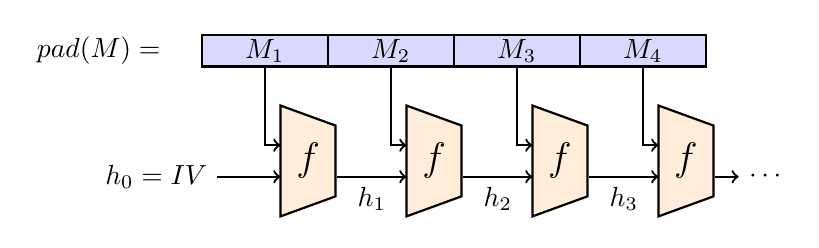
\begin{tikzpicture}[scale=0.4]
        \path[anchor=east] (-1,0.5) node {$pad(M)=$};
        \draw[fill=blue!15,thick,inner sep=2ex] (0,0) rectangle (16,1);
    
        %% Separations in the message
        \draw[thick] ++( 4,0) -- ++(0,1); \path (   2,0.5) node {$M_{1}$};
        \draw[thick] ++( 8,0) -- ++(0,1); \path ( 4+2,0.5) node {$M_{2}$};
        \draw[thick] ++(12,0) -- ++(0,1); \path ( 8+2,0.5) node {$M_{3}$};
        \draw[thick] ++(16,0) -- ++(0,1); \path (12+2,0.5) node {$M_{4}$};
    
        %% Compressions functions 
        \begin{scope}[shift={(0.5,-4)}]
            \node [draw,trapezium,trapezium left angle=70,trapezium right angle=70,minimum height=0.7cm,thick,fill=orange!15,shift={(1.15,0.4)},rotate=-90] 
            {\begin{sideways}\Large$f$\end{sideways}};
            \draw[->,thick] ++(1.5,+4) -- ++(0,-2.5) -- ++(0.5,0);
            \draw[->,thick] ++(0,0.5) node[left] {$h_{0}=IV$}-- ++(2,0);
        \end{scope}
    
        \begin{scope}[shift={(4.5,-4)}]
            \node [draw,trapezium,trapezium left angle=70,trapezium right angle=70,minimum height=0.7cm,thick,fill=orange!15,shift={(1.15,0.4)},rotate=-90] 
            {\begin{sideways}\Large$f$\end{sideways}};
            \draw[->,thick] ++(1.5,+4) -- ++(0,-2.5) -- ++(0.5,0);
            \draw[->,thick] ++(-0.2,0.5) -- node[below] {$h_{1}$} ++(2.2,0);
        \end{scope}
    
        \begin{scope}[shift={(8.5,-4)}]
            \node [draw,trapezium,trapezium left angle=70,trapezium right angle=70,minimum height=0.7cm,thick,fill=orange!15,shift={(1.15,0.4)},rotate=-90] 
            {\begin{sideways}\Large$f$\end{sideways}};
            \draw[->,thick] ++(1.5,+4) -- ++(0,-2.5) -- ++(0.5,0);
            \draw[->,thick] ++(-0.2,0.5) -- node[below] {$h_{2}$} ++(2.2,0);
        \end{scope}
    
        \begin{scope}[shift={(12.5,-4)}]
            \node [draw,trapezium,trapezium left angle=70,trapezium right angle=70,minimum height=0.7cm,thick,fill=orange!15,shift={(1.15,0.4)},rotate=-90] 
            {\begin{sideways}\Large$f$\end{sideways}};
            \draw[->,thick] ++(1.5,+4) -- ++(0,-2.5) -- ++(0.5,0);
            \draw[->,thick] ++(-0.2,0.5) -- node[below] {$h_{3}$} ++(2.2,0);
        \end{scope}
    
        \begin{scope}[shift={(16.5,-4)}]
            \draw[->,thick] ++(-0.2,0.5) -- ++(0.75,0) node[right] {$\cdots$} ;
        \end{scope}
    
    \end{tikzpicture}
    }
    \pause
    \resizebox{18em}{!}{
        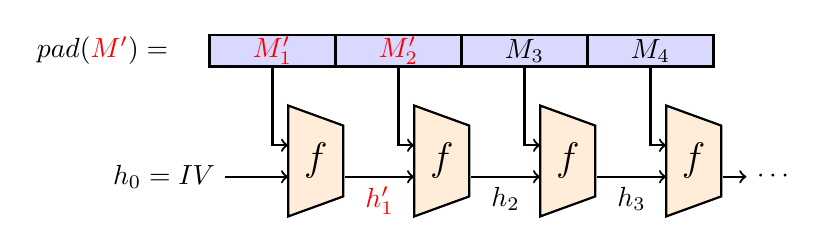
\begin{tikzpicture}[scale=0.4]
        	\path[anchor=east] (-1,0.5) node {$pad(\textcolor{red}{M'})=$};
        	\draw[fill=blue!15,thick,inner sep=2ex] (0,0) rectangle (16,1);
        
        	%% Separations in the message
        	\draw[thick] ++( 4,0) -- ++(0,1); \path (   2,0.5) node {$\textcolor{red}{M'_{1}}$};
        	\draw[thick] ++( 8,0) -- ++(0,1); \path ( 4+2,0.5) node {$\textcolor{red}{M'_{2}}$};
        	\draw[thick] ++(12,0) -- ++(0,1); \path ( 8+2,0.5) node {$M_{3}$};
        	\draw[thick] ++(16,0) -- ++(0,1); \path (12+2,0.5) node {$M_{4}$};
        
        	%% Compressions functions 
        	\begin{scope}[shift={(0.5,-4)}]
        		\node [draw,trapezium,trapezium left angle=70,trapezium right angle=70,minimum height=0.7cm,thick,fill=orange!15,shift={(1.15,0.4)},rotate=-90] 
        		{\begin{sideways}\Large$f$\end{sideways}};
        		\draw[->,thick] ++(1.5,+4) -- ++(0,-2.5) -- ++(0.5,0);
        		\draw[->,thick] ++(0,0.5) node[left] {$h_{0}=IV$}-- ++(2,0);
        	\end{scope}
        
        	\begin{scope}[shift={(4.5,-4)}]
        		\node [draw,trapezium,trapezium left angle=70,trapezium right angle=70,minimum height=0.7cm,thick,fill=orange!15,shift={(1.15,0.4)},rotate=-90] 
        		{\begin{sideways}\Large$f$\end{sideways}};
        		\draw[->,thick] ++(1.5,+4) -- ++(0,-2.5) -- ++(0.5,0);
        		\draw[->,thick] ++(-0.2,0.5) -- node[below] {$\textcolor{red}{h'_{1}}$} ++(2.2,0);
        	\end{scope}
        
        	\begin{scope}[shift={(8.5,-4)}]
        		\node [draw,trapezium,trapezium left angle=70,trapezium right angle=70,minimum height=0.7cm,thick,fill=orange!15,shift={(1.15,0.4)},rotate=-90] 
        		{\begin{sideways}\Large$f$\end{sideways}};
        		\draw[->,thick] ++(1.5,+4) -- ++(0,-2.5) -- ++(0.5,0);
        		\draw[->,thick] ++(-0.2,0.5) -- node[below] {$h_{2}$} ++(2.2,0);
        	\end{scope}
        
        	\begin{scope}[shift={(12.5,-4)}]
        		\node [draw,trapezium,trapezium left angle=70,trapezium right angle=70,minimum height=0.7cm,thick,fill=orange!15,shift={(1.15,0.4)},rotate=-90] 
        		{\begin{sideways}\Large$f$\end{sideways}};
        		\draw[->,thick] ++(1.5,+4) -- ++(0,-2.5) -- ++(0.5,0);
        		\draw[->,thick] ++(-0.2,0.5) -- node[below] {$h_{3}$} ++(2.2,0);
        	\end{scope}
        
        	\begin{scope}[shift={(16.5,-4)}]
        		\draw[->,thick] ++(-0.2,0.5) -- ++(0.75,0) node[right] {$\cdots$} ;
        	\end{scope}
            
        \end{tikzpicture}
    }
    \footnote{\cite{TikZ:for:Cryptographers}}
    \begin{outline}
        \1 Une collision pour $h_2$ entraînera une collision sur tous les états suivants
            \2[$\longrightarrow$] Si $md5(m)=md5(m')$, alors $md5(m||a) = md5(m'||a)$ 
        \pause
        \1 Dans notre cas :
            \2 Collision md5 pour $m$, $m'$ en quelques secondes \footnote{\url{https://github.com/cr-marcstevens/hashclash}}
            \pause
            \2 $2^{24}$ candidats $a$ pour pour avoir les 3 derniers bytes de $md5(m ||a)$ 
            \pause
            \2 On à gratuitement la même chose pour $md5(m' || a)$
            \pause
            \2 Ceci double les chances d'avoir une collision sur sha1
            \pause
            \2 Pourquoi s'arrêter là?
    \end{outline}
\end{frame}


%------------------------------------------------
%------------------------------------------------


\begin{frame}{Collisions multiples et md5}
\centering
    \resizebox{18em}{!}{
    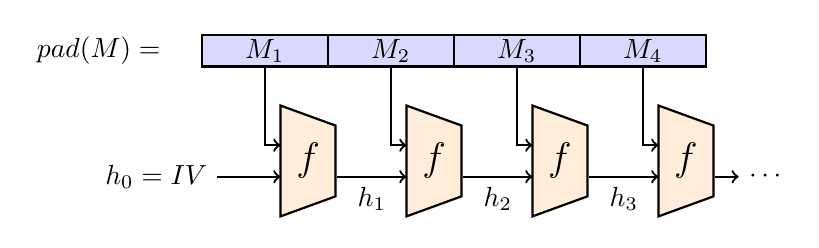
\begin{tikzpicture}[scale=0.4]
        \path[anchor=east] (-1,0.5) node {$pad(M)=$};
        \draw[fill=blue!15,thick,inner sep=2ex] (0,0) rectangle (16,1);
    
        %% Separations in the message
        \draw[thick] ++( 4,0) -- ++(0,1); \path (   2,0.5) node {$M_{1}$};
        \draw[thick] ++( 8,0) -- ++(0,1); \path ( 4+2,0.5) node {$M_{2}$};
        \draw[thick] ++(12,0) -- ++(0,1); \path ( 8+2,0.5) node {$M_{3}$};
        \draw[thick] ++(16,0) -- ++(0,1); \path (12+2,0.5) node {$M_{4}$};
    
        %% Compressions functions 
        \begin{scope}[shift={(0.5,-4)}]
            \node [draw,trapezium,trapezium left angle=70,trapezium right angle=70,minimum height=0.7cm,thick,fill=orange!15,shift={(1.15,0.4)},rotate=-90] 
            {\begin{sideways}\Large$f$\end{sideways}};
            \draw[->,thick] ++(1.5,+4) -- ++(0,-2.5) -- ++(0.5,0);
            \draw[->,thick] ++(0,0.5) node[left] {$h_{0}=IV$}-- ++(2,0);
        \end{scope}
    
        \begin{scope}[shift={(4.5,-4)}]
            \node [draw,trapezium,trapezium left angle=70,trapezium right angle=70,minimum height=0.7cm,thick,fill=orange!15,shift={(1.15,0.4)},rotate=-90] 
            {\begin{sideways}\Large$f$\end{sideways}};
            \draw[->,thick] ++(1.5,+4) -- ++(0,-2.5) -- ++(0.5,0);
            \draw[->,thick] ++(-0.2,0.5) -- node[below] {$h_{1}$} ++(2.2,0);
        \end{scope}
    
        \begin{scope}[shift={(8.5,-4)}]
            \node [draw,trapezium,trapezium left angle=70,trapezium right angle=70,minimum height=0.7cm,thick,fill=orange!15,shift={(1.15,0.4)},rotate=-90] 
            {\begin{sideways}\Large$f$\end{sideways}};
            \draw[->,thick] ++(1.5,+4) -- ++(0,-2.5) -- ++(0.5,0);
            \draw[->,thick] ++(-0.2,0.5) -- node[below] {$h_{2}$} ++(2.2,0);
        \end{scope}
    
        \begin{scope}[shift={(12.5,-4)}]
            \node [draw,trapezium,trapezium left angle=70,trapezium right angle=70,minimum height=0.7cm,thick,fill=orange!15,shift={(1.15,0.4)},rotate=-90] 
            {\begin{sideways}\Large$f$\end{sideways}};
            \draw[->,thick] ++(1.5,+4) -- ++(0,-2.5) -- ++(0.5,0);
            \draw[->,thick] ++(-0.2,0.5) -- node[below] {$h_{3}$} ++(2.2,0);
        \end{scope}
    
        \begin{scope}[shift={(16.5,-4)}]
            \draw[->,thick] ++(-0.2,0.5) -- ++(0.75,0) node[right] {$\cdots$} ;
        \end{scope}
    \end{tikzpicture}
    }

    \pause
    
    \begin{itemize}
        \item Pour IV fixé, trouver $m_1$ et $m'_1$ en collision sur $h_1$
        \pause
        \item Pour $h_1$ trouver $m_2$ et $m'_2$ en collision sur $h_2$
        \pause
        \item etc
    \end{itemize}
    \pause
    \resizebox{25em}{!}{
        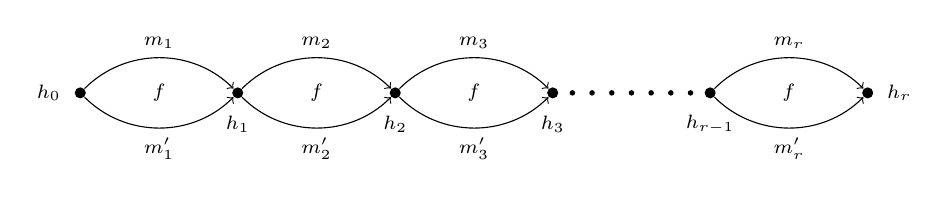
\begin{tikzpicture}[scale=1]
        
           \draw (0,0) node[fill,circle,inner sep=0pt,minimum size=4pt] (a1) {};%
           \draw (2,0) node[fill,circle,inner sep=0pt,minimum size=4pt] (a2) {};%
           \draw (4,0) node[fill,circle,inner sep=0pt,minimum size=4pt] (a3) {};%
           \draw (6,0) node[fill,circle,inner sep=0pt,minimum size=4pt] (a4) {};%
        
           \draw (6.25,0) node[fill,circle,inner sep=0pt,minimum size=2pt] (b0) {};%
           \draw (6.5,0) node[fill,circle,inner sep=0pt,minimum size=2pt] (b1) {};%
           \draw (6.75,0) node[fill,circle,inner sep=0pt,minimum size=2pt] (b2) {};%
           \draw (7,0) node[fill,circle,inner sep=0pt,minimum size=2pt] (b3) {};%
           \draw (7.25,0) node[fill,circle,inner sep=0pt,minimum size=2pt] (b4) {};%
           \draw (7.5,0) node[fill,circle,inner sep=0pt,minimum size=2pt] (b5) {};%
           \draw (7.75,0) node[fill,circle,inner sep=0pt,minimum size=2pt] (b6) {};%
        
           \draw (8,0) node[fill,circle,inner sep=0pt,minimum size=4pt] (a5) {};%
           \draw (10,0) node[fill,circle,inner sep=0pt,minimum size=4pt] (a6) {};%
          
           \draw[->] (a1) edge[out= 45, in= 3*45] node[above]{\scriptsize $m_{1}$} (a2);
           \draw[->] (a1) edge[out=-45, in=-3*45] node[below]{\scriptsize $m'_{1}$} (a2);
          
           \draw[->] (a2) edge[out= 45, in= 3*45] node[above]{\scriptsize $m_{2}$} (a3);
           \draw[->] (a2) edge[out=-45, in=-3*45] node[below]{\scriptsize $m'_{2}$} (a3);
          
           \draw[->] (a3) edge[out= 45, in= 3*45] node[above]{\scriptsize $m_{3}$} (a4);
           \draw[->] (a3) edge[out=-45, in=-3*45] node[below]{\scriptsize $m'_{3}$} (a4);
           
           \draw[->] (a5) edge[out= 45, in= 3*45] node[above]{\scriptsize $m_{r}$} (a6);
           \draw[->] (a5) edge[out=-45, in=-3*45] node[below]{\scriptsize $m'_{r}$} (a6);
           
           \path (1,0) node {\scriptsize $f$};
           \path (3,0) node {\scriptsize $f$};
           \path (5,0) node {\scriptsize $f$};
           \path (9,0) node {\scriptsize $f$};
           
          
           \path (-0.4,0) node {\scriptsize $h_{0}$};
           \path (2,-0.4) node {\scriptsize $h_{1}$};
           \path (4,-0.4) node {\scriptsize $h_{2}$};
           \path (6,-0.4) node {\scriptsize $h_{3}$};
           \path (8,-0.4) node {\scriptsize $h_{r-1}$};
           \path (10+0.4,0) node {\scriptsize $h_{r}$};
        
        \end{tikzpicture}
    }
    \begin{outline}
        \1 $2^{r}$ collisions sur $h_r$ générées pour le prix de $r$
        \pause
        \1 Dans notre cas
            \2 On génère facilement $2^{24}$ collisions $md5(x_1)= \cdots = md5(x_{2^{24}})$
            \pause
            \2 On itère sur $2^{24}$ valeurs de $a$ jusqu'à avoir la collision sur $md5(x_1 || a)$
            \pause
            \2 Statistiquement, il y a une collision pour au moins un des $sha1(x_i || a)$  $\flag$
    \end{outline}
\end{frame}

\subsection{Kyber et les anneaux quotients}
\begin{frame}{Kyber et les anneaux quotients}
    \large{\centerline{\textbf{}}}

\end{frame}

%------------------------------------------------
%------------------------------------------------

\begin{frame}{Kzber \FiveStar \FiveStar\FiveStar \hfill 25 résolutions}
    \begin{columns}[c]
        \column{.45\textwidth}
        \begin{center}                  
            
\includegraphics[width=0.9\textwidth]{img/meme/kyber-intro.png}
        \end{center}

        \column{.65\textwidth} % 
           \begin{outline}
                \1 Objectifs : 
                    \2 Récupérer $\u{k}$ sur 128 bits  chiffré via Kyber
                \1 Données :
                    \2 La clef publique $\k{A}$ et $\k{t}$
                    \2 Le chiffré $E(\u{k})$
                    \2 Le code source
           \end{outline}
    \end{columns}
\end{frame}

%------------------------------------------------
%------------------------------------------------

\begin{frame}{Kyber / ML-KEM (le vrai)}
PQ-KEM (chiffrement asymétrique) standardisé par le NIST
\pause
   \begin{block}{\only<3->{Ring/Module }Learning with Errors (\only<3->{R/M}LwE)}
   Soit $\k{A}\in\mathbb{Z}_q^{k\times k}$.
       \begin{itemize}
        \item Facile de récupérer $\u{s}\in\mathbb{Z}_q^k$ sachant $\k{t}=\k{A}.\u{s}$ (Interpolation)
        \pause
        \item Difficile  de récupérer $\u{s}\in\mathbb{Z}_q^k$ sachant $\k{t}=\k{A}.\u{s}+\u{e}$ où $\u{e}\in\mathbb{Z}_q^{k}$ est petit ($|\u{e}|<\eta$)
        \pause 
        \item Même chose dans $\mathcal{R}_q^k = \left(\mathbb{Z}_q[X]/\left<\phi\right>\right)^k$, et $\phi$ de degré $n$
       \end{itemize}
   \end{block}
   \pause
   \begin{table}
        \begin{tabular}{c|c|c|c|c}
            Nom       & n   & k & q    & $\eta$ \\
            \hline
            Kyber512  & 256 & 2 & 3329 & 2\\
            Kyber768  & 256 & 3 & 3329 & 2\\
            Kyber1024 & 256 & 4 & 3329 & 2\\
        \end{tabular}
    \end{table}
    \pause 
    $\mathcal{R}_q = \mathbb{Z}_q[X]/(X^n+1)$
\end{frame}

\begin{frame}{Algorithmes de Kyber}
    \begin{columns}[c]
        \column{.5\textwidth}
            \begin{outline}
                \1 \textbf{Keygen} : $\k{t} = \k{A}. \u{s}+\u{e}$ 
                    \2 Clef privée $(\u{s})$
                    \2 Clef publique $(\k{A},\k{t})$
                \pause
                \1 \textbf{Chiffrement $m$} : 
                    \2 $\left\{
                \begin{array}{c c l}
                   \k{u} & = & \k{A}^T\u{r} + \u{e_1}\\
                   \k{v} & = & \k{t}^T\u{r}+\u{e_2} + m\\
                \end{array}
                \right.$
                \pause
                \1 \textbf{Déchiffrement $(u,v)$} : 
                    \2 $\k{v}-\u{s}^T\k{u} = m +\u{e}^T\u{r}+\u{e_2} + \u{s}^T\u{e_1} = m + \u{e_3}$
                \end{outline}
        \column{.65\textwidth} % 
        \begin{center}   
            \only<4>{
                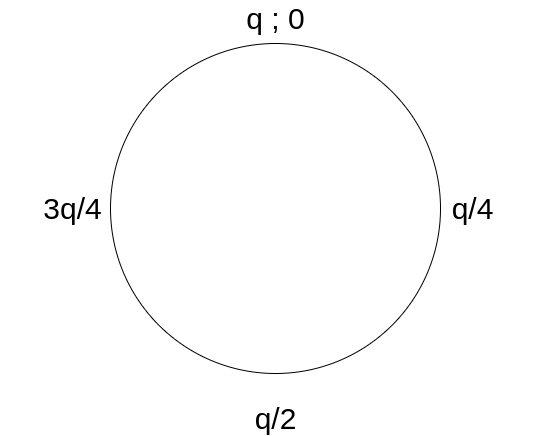
\includegraphics[width=0.8\textwidth]{img/crypto/kyber/kyber-modulo.png}
            }
            \only<5>{
                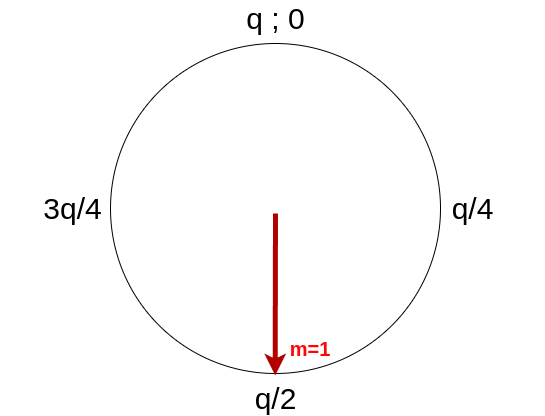
\includegraphics[width=0.8\textwidth]{img/crypto/kyber/kyber-chose_m.png}
            }
            \only<6>{
                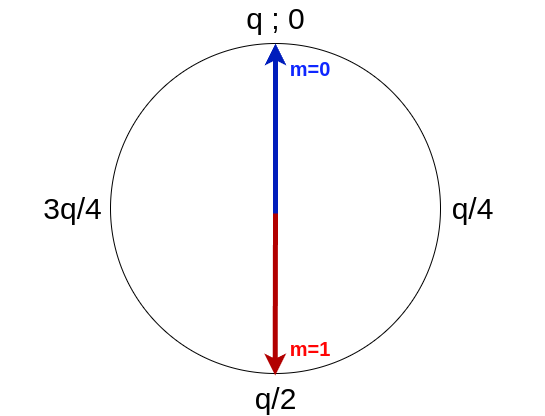
\includegraphics[width=0.8\textwidth]{img/crypto/kyber/kyber-1 or 0.png}
            }
            \only<7>{
                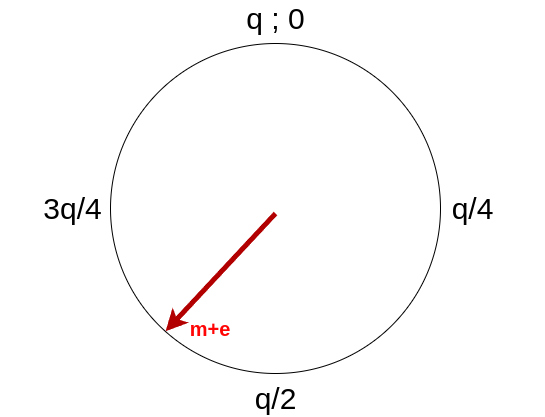
\includegraphics[width=0.8\textwidth]{img/crypto/kyber/kyber-add error.png}
            }
            \only<8->{
                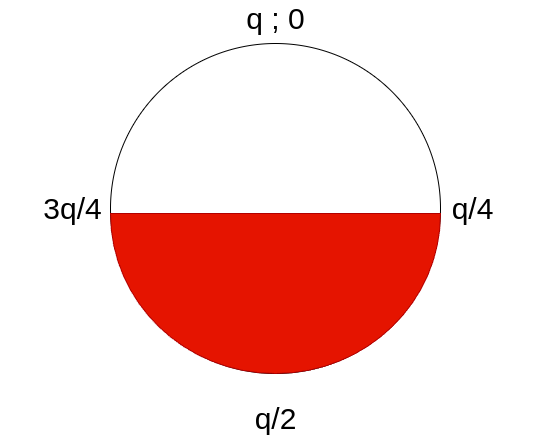
\includegraphics[width=0.8\textwidth]{img/crypto/kyber/kyber-decrypt.png}
            }
        \end{center}
   \end{columns}
   \pause
   $m$ est un polynôme de $\mathcal{R}_q$ (e.g $0101$ devient $0+\frac{q}{2}x+0x^2+\frac{q}{2}x^3$)
\end{frame}

\begin{frame}{Retour au challenge : La (les?) typos}
    \begin{outline}
        \1 $E(m_0),\dots,E(m_k)$ au lieu de $E(m_0,\dots,m_k)$
            \2 $m$ est le polynôme constant 0 ou $q/2$

        \vspace{0.2cm}
        \pause
        
        \1 Travail modulo $X^n\textbf{-}1$ (au lieu de $X^n+1$) qui admet des racines dans $\mathbb{Z}_q$ 
        \pause
            \2 $P\mapsto P(1)$ est un morphisme d'anneau sur $\mathcal{R}_q$ % $\longrightarrow$ somme des coefficients
	    	\3 C'est le morphisme $P \mapsto P \mod X-1$

            \vspace{0.1cm}
            \pause
            
            \2  $\k{v}(1) = \left[\k{t_0}(1),\,\k{t_1}(1)\right]\bullet \left[\u{r_0}(1),\,\u{r_1}(1)\right]^{T}+\u{e_2}(1) + m(1)$ \pause $\in[-q/2,q/2]$ 
            \pause
                \3 $\k{v}(1) = \k{0}+\u{e_2}(1) + m$  avec probabilité $1/q^2$ \hfill ($\sim\frac{1}{11\,082\,241}$)
                \pause
                \3 $\k{v}(1) = \k{\epsilon}\u{r_0}(1)+\k{\epsilon}\u{r_1}(1)+\u{e_2}(1) + m$  avec probabilité $\epsilon^2/q^2$ \hfill ($\sim\frac{1}{12\,313}$)
                \pause
                %\3 Bruteforce des valeurs de $\u{r_0}(1),\u{r_1}(1)$ (à réinjecter dans $\k{v}=\k{A}\cdot\u{r}+\u{e_2}$)

            \vspace{0.1cm}
            \pause
            
            \2 $P\mapsto P(-1)$ est aussi un morphisme d'anneau \hfill ($\sim\frac{1}{6\,156}$)
	    	\3 C'est le morphisme $P \mapsto P \mod X+1$

            \vspace{0.1cm}
            \pause
            
            \2 $X^{256}-1$ à exactement 256 racines dans $\mathbb{Z}_q$ (et $X^{256}+1$ n'en a pas)
		\3 Difficile à exploiter car $\u{e_2}(r)$ est grand
		
		\pause
	    \2 $X^{256}-1$ est divisible par $X^{2^k}-1$  (et $X^{256}+1$ n'en a pas)\hfill ($\sim\frac{1}{96}$)
        \vspace{0.2cm}
        \pause

        \1 On peut générer des instances du problème jusqu'à avoir la solution via au moins l'un de ces morphismes $\flag$

    \end{outline}
\end{frame}

\subsection{Analyse différentielle et boomerang}
\begin{frame}{Analyse différentielle et boomerang}
    \large{\centerline{\textbf{Attaque sur SbPN}}}

\end{frame}

%------------------------------------------------
%------------------------------------------------

\begin{frame}{Le retour de Jafar \FiveStar \FiveStar \hfill \textcolor{red}{8 résolutions :(}}
    \begin{columns}[c]
        \column{.45\textwidth}
        \begin{center}                  
            
\includegraphics[width=0.9\textwidth]{img/meme/jafar-intro.png}
        \end{center}

        \column{.65\textwidth} % 
           \begin{outline}
                \1 Objectifs : 
                    \2 Forger un couple clair / chiffré sans connaître la clef

                    \pause 
                \1 Données
                    \2 Exactement 3 oracles de chiffrement / déchiffrement
                    \2 Le code source
           \end{outline}
    \end{columns}
\end{frame}


%------------------------------------------------
%------------------------------------------------

\begin{frame}{Le cipher Jafar}
  \begin{columns}[c]
        \column{.50\textwidth} %
             \begin{center}                  
                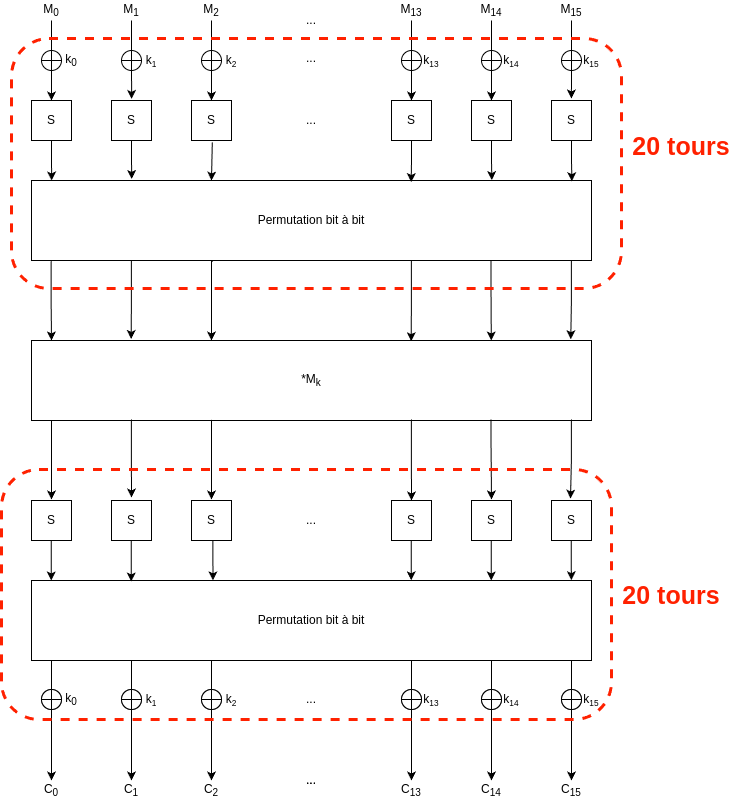
\includegraphics[width=0.9\textwidth]{img/crypto/jafar/jafar-scheme.png}
            \end{center}
        \column{.50\textwidth}
           \begin{outline}
                \1 40 tours au total
                \pause
                \1 Pas de tour de clef
                \pause
                \1 Tout est linéaire à part la SBox
                \pause
                \begin{center}                  
                 
\includegraphics[width=0.9\textwidth]{img/meme/jafar-meme.png}
                \end{center}
                \hfill \tiny{@bluesheet}
           \end{outline}
    \end{columns}
\end{frame}

%------------------------------------------------
%------------------------------------------------

\begin{frame}[fragile] % <---
\frametitle{Fausse piste : la permutation}
  \begin{columns}[c]

    \column{.45\textwidth}
        \begin{lstlisting}[language=Python]
P_Perm = Permutation(P)
P_perm.show("braid")
P_perm.fixed_points()
P_perm.cycle_tuples()
        \end{lstlisting}

        \begin{itemize}
            \item Deux points fixes (2 et 94)
            \item Trois cycles non triviaux de taille 82, 31, 13
        \end{itemize}
    \column{.40\textwidth} %
        \begin{center}                  
            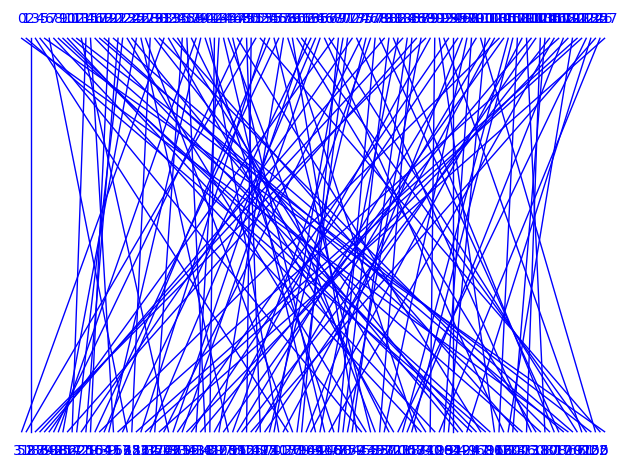
\includegraphics[width=0.9\textwidth]{img/crypto/jafar/permutation.png}
        \end{center}
    \end{columns}

\end{frame}


\begin{frame}[fragile] % <---
\frametitle{Analyse de la SBox}
  \begin{columns}[c]
    \column{.70\textwidth}
        \begin{lstlisting}[language=Python]
from sage.crypto.sbox import SBox
sb = SBox(S)
sb.difference_distribution_table()
\end{lstlisting}
        \begin{outline}
            \1 DDT[a,b] := Probabilité que $S[x\oplus a] = S[x]\oplus b$
            
            \only<2->{
                \2[$\longrightarrow$] 4 différentielles par Sbox: $(0\mapsto 0)$ ,$(24\mapsto 129)$, $(74\mapsto 7)$, $(82 \mapsto 134)$
                }
            \only<3->{
            \1 16 octets $\Rightarrow$ $2^{32}$ différentielles à tester
            }
        \end{outline}
    \column{.30\textwidth} %
        \begin{center}                  
            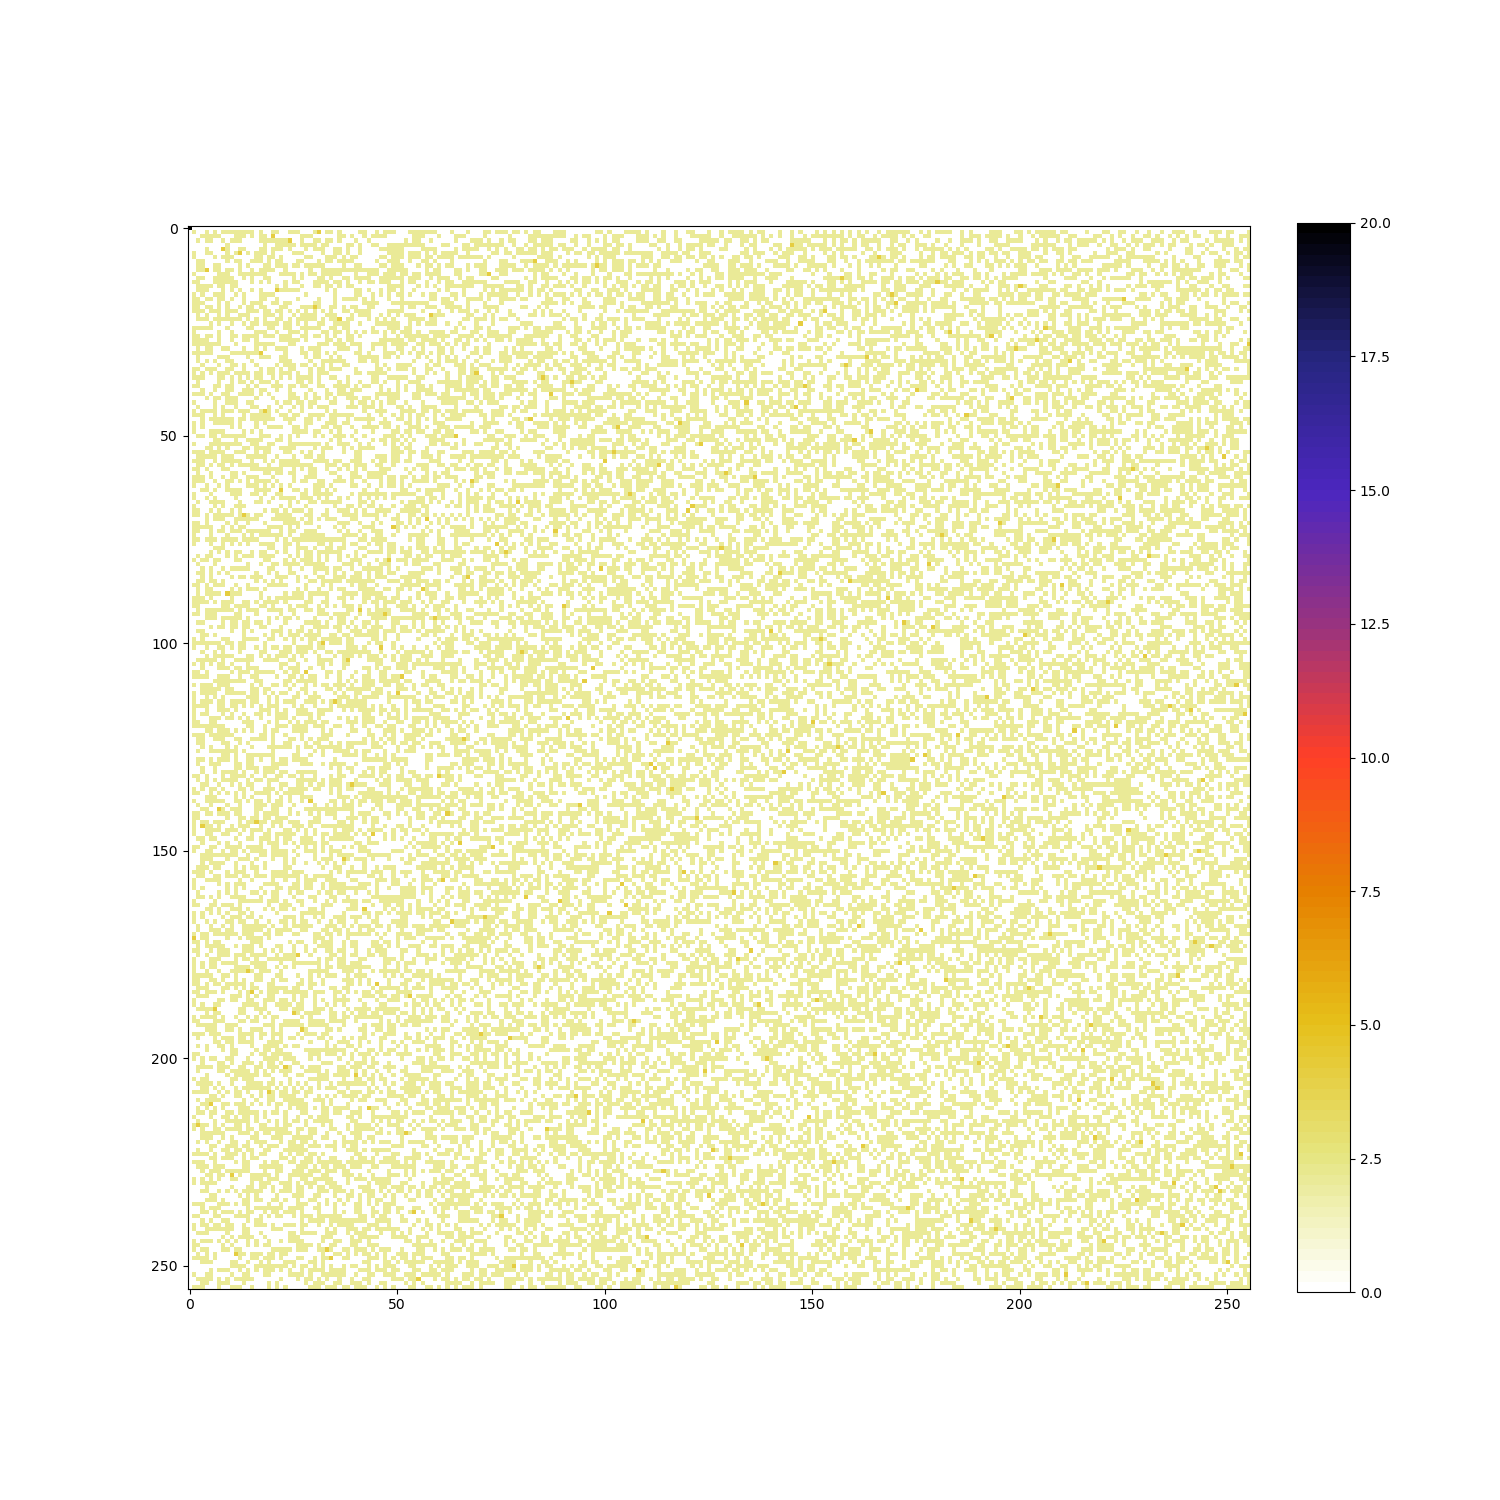
\includegraphics[trim=30pt 140pt 30pt 140pt, clip, width=0.9\textwidth]{img/crypto/jafar/AES-ddt.png}
        \end{center}
        \pause 
        \begin{center}                  
            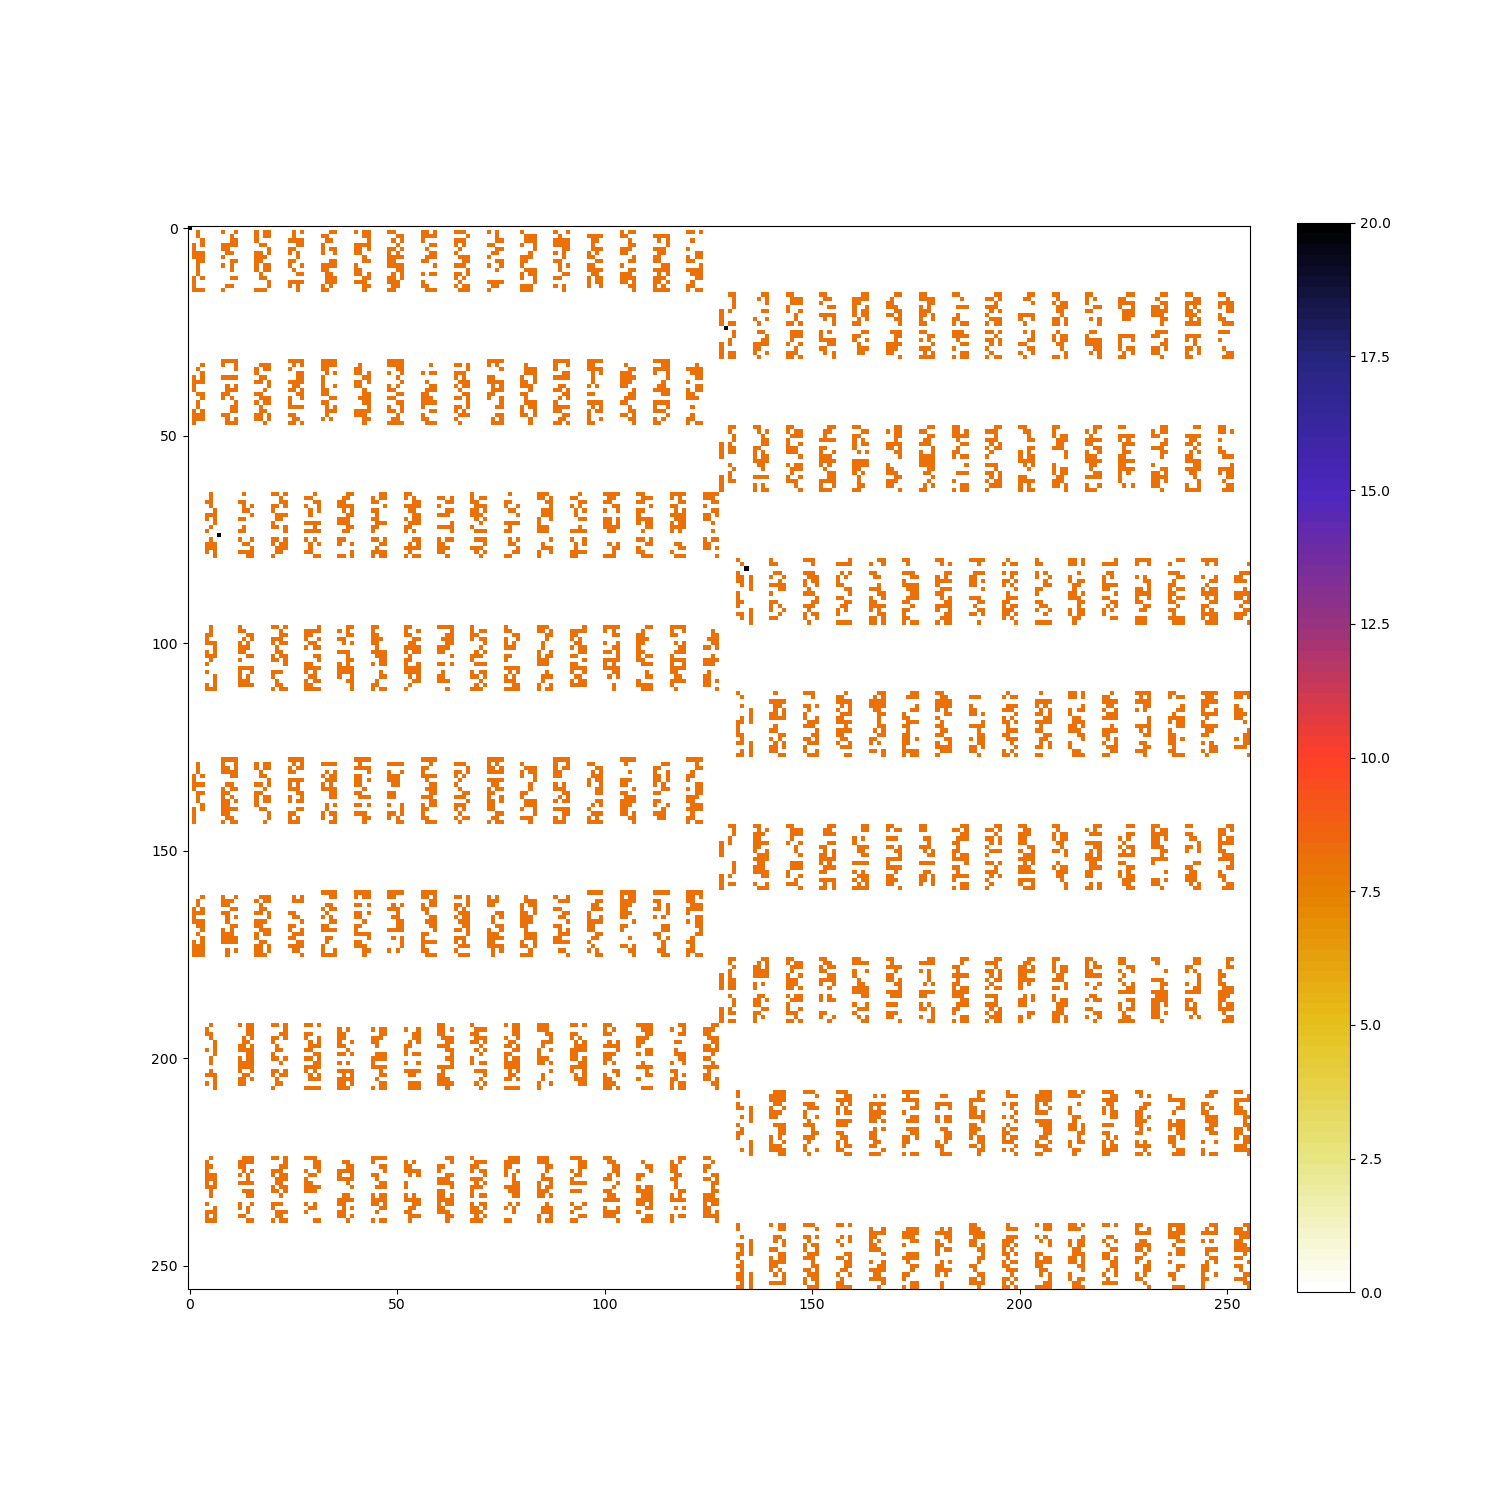
\includegraphics[trim=30pt 30pt 30pt 100pt, clip, width=0.9\textwidth]{img/crypto/jafar/sbox-ddt.png}
        \end{center}
    \end{columns}

\end{frame}



\begin{frame}{Introduire une différentielle}
        \begin{center}                  
            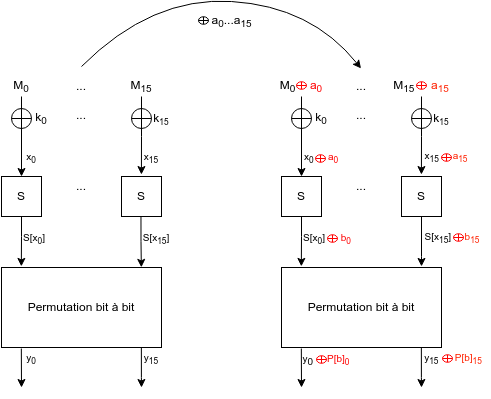
\includegraphics[width=0.53\textwidth]{img/crypto/jafar/auto/1round.png}
        \end{center}
        \pause
    \begin{itemize}
        \item $D_{in}=[0, 82, 0, 24, 0, 0, 0, 82, 0, 0, 0, 0, 0, 0, 0, 0]$
        \item $D_{out}=[0, 0, 0, 0, 0, 74, 0, 0, 0, 0, 24, 0, 0, 74, 0, 0]$
    \end{itemize}

\end{frame}


\begin{frame}{Sur 20 rounds}
        \begin{center}                  
            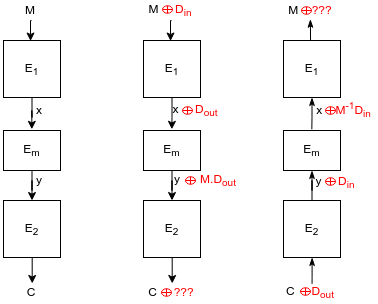
\includegraphics[width=0.6\textwidth]{img/crypto/jafar/auto/first-try.png}
        \end{center}
\end{frame}

\begin{frame}{Introduction au boomerang \only<6>{\flag}}
    \only<1>{
        \begin{center}                  
            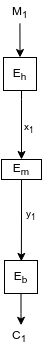
\includegraphics[scale=0.5]{img/crypto/jafar/auto/boomerang-1.png}
        \end{center}
    }
    \only<2>{
        \begin{center}                  
            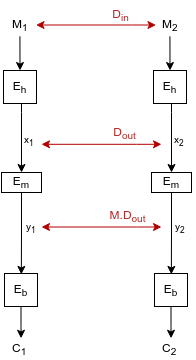
\includegraphics[scale=0.5]{img/crypto/jafar/auto/boomerang-2.png}
        \end{center}
    }
    \only<3>{
        \begin{center}                  
            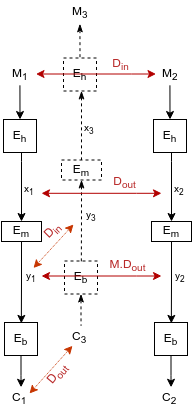
\includegraphics[scale=0.5]{img/crypto/jafar/auto/boomerang-3.png}
        \end{center}
    }
    \only<4>{
        \begin{center}                  
            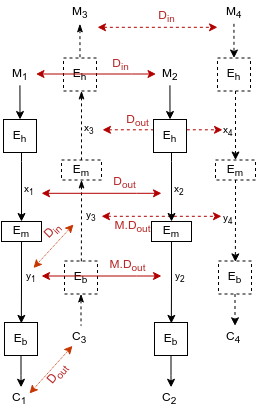
\includegraphics[scale=0.5]{img/crypto/jafar/auto/boomerang-4.png}
        \end{center}
    }
    \only<5->{
        \begin{center}                  
            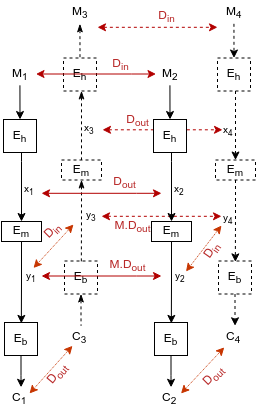
\includegraphics[scale=0.5]{img/crypto/jafar/auto/boomerang-5.png}
        \end{center}
    }

\end{frame}
\subsection{Le schéma multivarié UOV}
\begin{frame}{Le schéma multivarié UOV}
    \large{\centerline{\textbf{Comment faire une (mauvaise) vinaigrette}}}
     \centering
    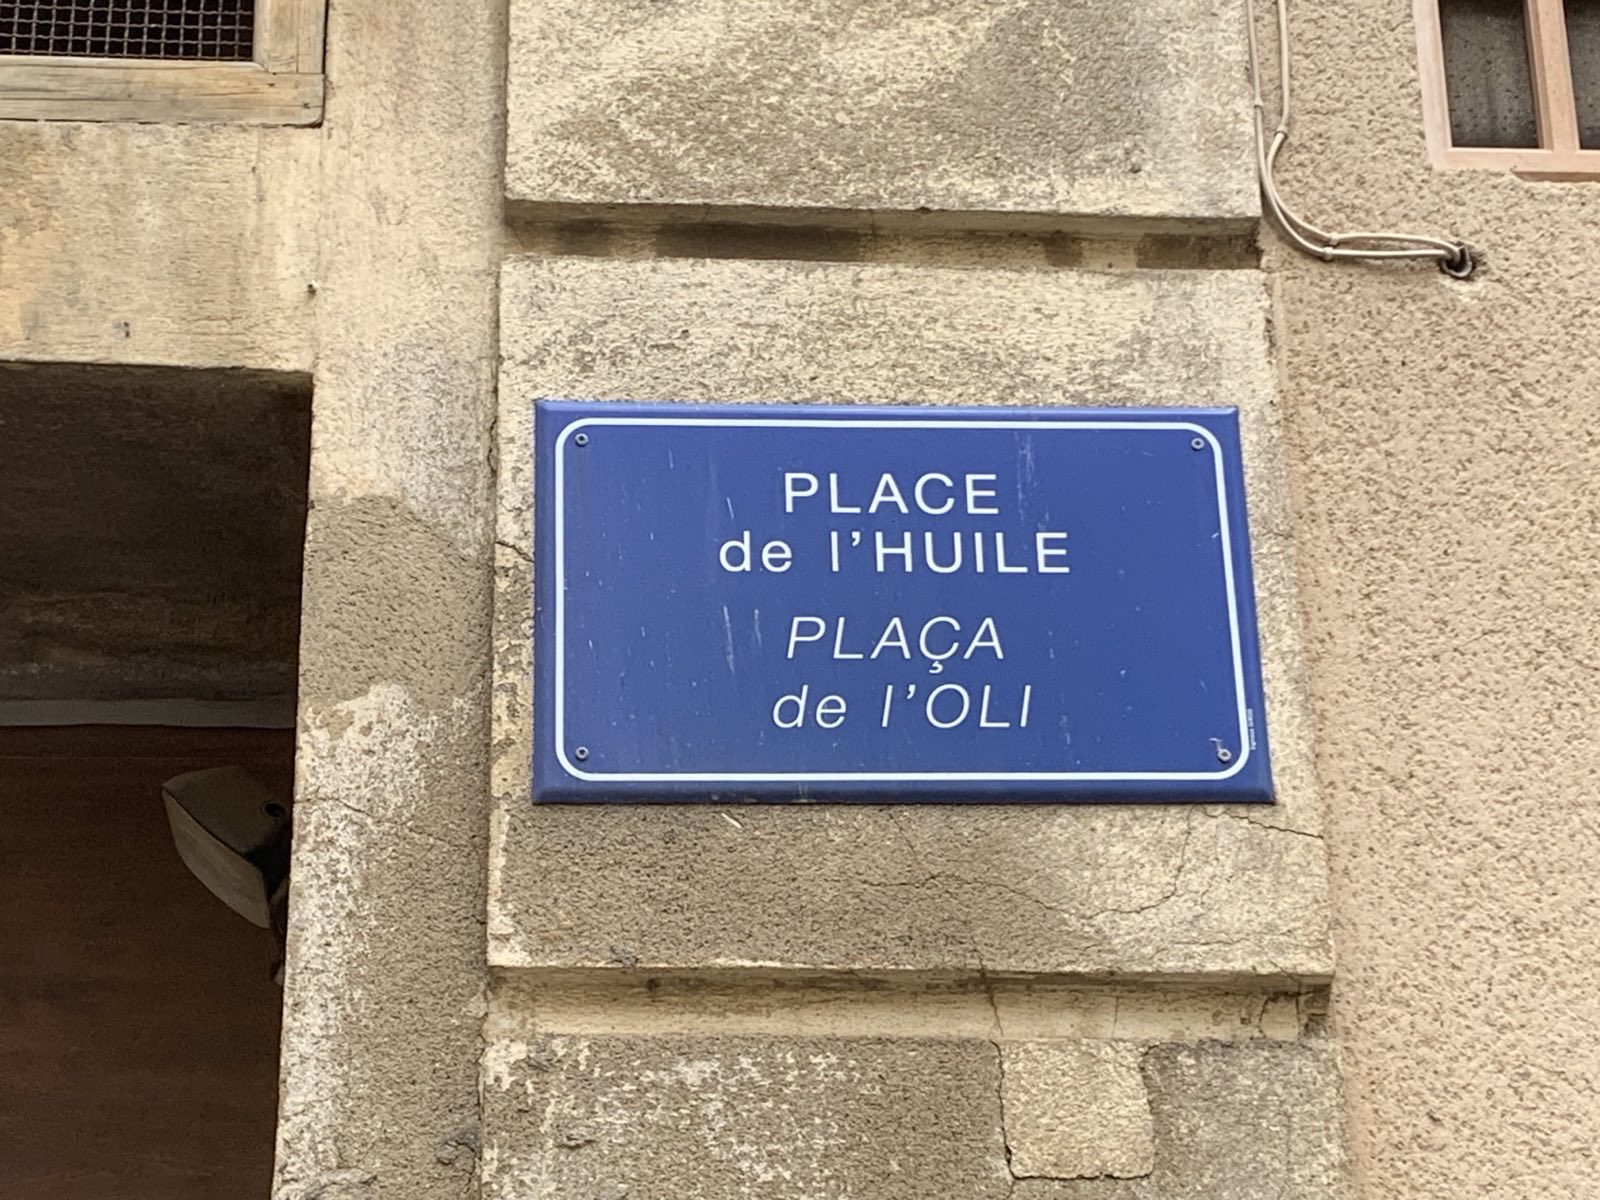
\includegraphics[trim=12cm 8cm 8cm 8cm, clip, width=0.5\linewidth]{img/meme/UOV-vac.jpg}
\end{frame}

%------------------------------------------------
%------------------------------------------------

\begin{frame}{Ça tourne au vinaigre \FiveStar\FiveStar\FiveStar \hfill 9 résolutions}
    \begin{columns}[c]
        \column{.55\textwidth}
        \begin{center}                  
            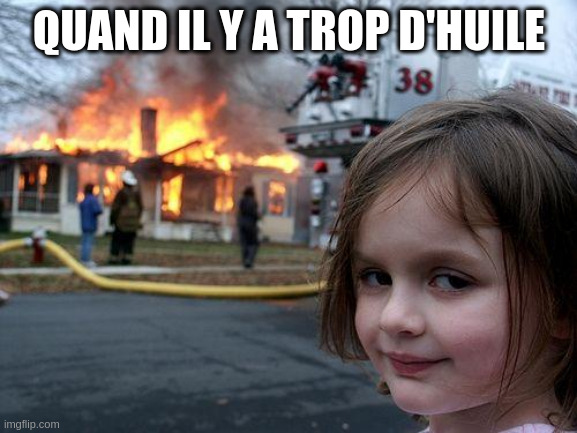
\includegraphics[width=0.9\textwidth]{img/meme/uov-intro.png}
        \end{center}

        \column{.45\textwidth} % 
           \begin{outline}
               \1 Objectifs :
                \2 Forger une signature valide
                \2 Sans la clef privée
                \pause
                \2 \textcolor{red}{Sans la clef publique}
                \pause
               \1 Données :
                    \2 1600 signatures

           \end{outline}
    \end{columns}
\end{frame}

%------------------------------------------------
%------------------------------------------------

%------------------------------------------------
%------------------------------------------------

\begin{frame}{Sur les représentations des fonctions quadratiques}
    \begin{columns}[c]
        \column{.50\textwidth}

            \begin{block}{Fonction quadratique}
                $f(x_1,\dots,x_n) = $
                \only<1>{
                    $\underset{i\leq j}{\displaystyle\sum} a_{ij}x_ix_j$ 
                }
                \only<2->{
                    \colorbox{blue!20}{$\underset{i\leq j}{\displaystyle\sum}a_{ij}x_ix_j$}
                }
                $ + $
                \only<1>{
                    $\underset{i}{\displaystyle\sum} b_{i}x_i$
                }
                \only<2->{
                    \colorbox{red!20}{$\underset{i}{\displaystyle\sum} b_{i}x_i$}
                }
                $ +\, c$
                \only<2->{
                    \\
                    \hspace{2.55cm}
                        \text{\scriptsize\color{blue!60} (quadratique)}
                    \hspace{0.65cm}
                        \text{\scriptsize\color{red!60} (linéaire)}
                }
            \end{block}
            \pause
            \begin{block}{Forme quadratique}             
                $f'(\textbf{x},\textbf{x}) = \underset{i\leq j}{\displaystyle\sum} a_{ij}x_i x_j$ \pause $= \textbf{x}^T \textbf{A} \textbf{x}$
            \end{block}

        \column{.45\textwidth}
            \only<3>{
            \begin{figure}
                \centering
                \includegraphics[width=5cm]{img/crypto/UOV/quadratic.png}
                \begin{tikzpicture}[overlay, remember picture]
                \end{tikzpicture}
                \captionsetup{labelformat=empty} % Removes the 'Figure' label
                \caption{Représentation matricielle d'une forme quadratique}

            \end{figure}
            }
            \only<4->{
                \begin{figure}
                \begin{tikzpicture}
                
                    \node[anchor=south west,inner sep=0] (image) at (0,0) {\includegraphics[width=5cm]{img/crypto/UOV/quadratic.png}};
                    \begin{scope}[x={(image.south east)}, y={(image.north west)}]
                        % Adjust these coordinates (0–1 range) to point to your (i,j) coefficient
                        \def\x{0.7}
                        \def\y{0.6}
                        \def\size{0.01}
                
                        % Draw square around pixel
                        \draw[red, line width=1.5mm] (\x-\size, \y-\size) rectangle (\x+\size, \y+\size);
                
                        % Axis labels
                        \node[above=2pt, xshift=\x*5cm, text=red] at (image.north west) {$j$};
                        \node[right=2pt, yshift=\y*5cm, text=red] at (image.south east) {$i$};
                            \node[red, right=\x*2.5cm, yshift=\y*2.5cm] {$a_{ij}x_ix_j$};
                    \end{scope}
            \end{tikzpicture}
            \captionsetup{labelformat=empty} % Removes the 'Figure' label
            \caption{Représentation matricielle d'une forme quadratique}
            \end{figure}
        }
    \end{columns}

\end{frame}

\begin{frame}{Sur les formes bilinéaires}

$f(x_1,\dots,x_n) = \underset{i\leq j}{\displaystyle\sum} a_{ij}x_ix_j + \underset{i}{\displaystyle\sum} b_{i}x_i + c$
    \begin{block}{Forme bilinéaire}             
        $f'(\textbf{x},\textbf{y}) = \underset{i\leq j}{\displaystyle\sum} a_{ij}x_i y_j$ \pause $= \textbf{x}^T \textbf{G} \textbf{y}$ \pause \hfill $/!\backslash$ $\textbf{}G$ est de taille maximale
    \end{block}
    \pause
    \begin{itemize}
        \item Pour $\textbf{y}$ fixé, une équation en $\textbf{x}$ est linéaire (et vice versa)
    \end{itemize}
    \pause
    \begin{block}{Composition}
        $f'(\textbf{x},\textbf{y})=f(\textbf{x}+\textbf{y})-f(\textbf{x}) - f(\textbf{y})+f(\textbf{0})$ est une forme bilinéaire symétrique
    \end{block}

    \begin{itemize}
      \item  Les parties linéaires et constantes se simplifient
      \item $(\textbf{x}+\textbf{y})^T \textbf{A}(\textbf{x}+\textbf{y}) = \textbf{x}^T\textbf{A}\textbf{x}+\textbf{y}^T\textbf{A}\textbf{y}+\textbf{x}^T(\textbf{A}+\textbf{A}^T)\textbf{y}$
    \end{itemize}
    
\end{frame}

\begin{frame}{Une signature via UOV (Unbalanced Oil and Vinegar)}
    
    \begin{block}{La clef publique UOV}
        $\mathcal{Q}=(\mathcal{Q}_1,\dots,\mathcal{Q}_h)$ des fonctions quadratiques à n variables

        $\mathcal{Q}_i(\textbf{y}) = \textbf{y}^T\textbf{A}_i\textbf{y} + \textbf{b}_i^T\textbf{y} + c_i $
    \end{block}
    \pause
    La signature de $\textbf{t}=(t_1,\dots,t_h)$ est une solution $\textbf{y}=(y_1,\dots,y_n)$ du système $\mathcal{Q}(\textbf{y})=\textbf{t}$ :
    \[\left\{
    \begin{array}{c}
       \mathcal{Q}_1(\textbf{y}) =  \mathcal{Q}_1(y_1,\dots,y_n) = t_1 \\
       \vdots \\
       \mathcal{Q}_h(\textbf{y}) =  \mathcal{Q}_h(y_1,\dots,y_n) = t_h \\
    \end{array}
    \right.\]
    \pause
    \begin{block}{Difficulté du problème UOV}
        Pour des bonnes valeurs de $h$, $v$ et $n=h+v$ , il est difficile de résoudre un tel système quadratique quelconque.
    \end{block}
    \pause
    Sans clef privée, il est difficile de signer un message
\end{frame}

\begin{frame}{La trapdoor d'UOV}
$\mathbb{F}_q^n=\mathbb{F}_q^h \oplus\mathbb{F}_q^v = \mathcal{H}\oplus\mathcal{V}$ (huile + vinaigre) $\pause \Rightarrow$ $\textbf{x} =(x_1,\dots,x_h,x_{h+1},\dots,x_{h+v}) = (\mathbf{x}_\mathcal{H},\mathbf{x}_\mathcal{V})$
    \pause
    \begin{columns}
        \column{.45\textwidth}
            \begin{figure}
                \begin{tikzpicture}
                
                    \node[anchor=south west,inner sep=0] (image) at (0,0) {\includegraphics[width=3cm]{img/crypto/UOV/quadratic.png}};
                    \begin{scope}[x={(image.south east)}, y={(image.north west)}]
                        % Adjust these coordinates (0–1 range) to point to your (i,j) coefficient
                        \def\x{0.7}
                        \def\y{0.6}
                        \def\size{0.01}
                
                        % Draw square around pixel
                        \draw[red, line width=1.5mm] (\x-\size, \y-\size) rectangle (\x+\size, \y+\size);
                
                        % Axis labels
                        \node[above=2pt, xshift=\x*3cm, text=red] at (image.north west) {$j$};
                        \node[right=2pt, yshift=\y*3cm, text=red] at (image.south east) {$i$};
                            \node[red, right=\x*1cm, yshift=\y*1cm] {$a_{ij}y_iy_j$};
                    \end{scope}
            \end{tikzpicture}
            \captionsetup{labelformat=empty} % Removes the 'Figure' label
            \caption{Partie quadratique de $\mathcal{Q}_i$ publique}
            \end{figure}
        \pause
        \column{.05\textwidth}
        $\overset{\mathbf{y}=\mathcal{S}(\mathbf{x})}{\Leftarrow}$
        \column{.45\textwidth}
            \begin{figure}
                \begin{tikzpicture}
                
                    \node[anchor=south west,inner sep=0] (image) at (0,0) {\includegraphics[width=3cm]{img/crypto/UOV/trapdoor.png}};
                    \begin{scope}[x={(image.south east)}, y={(image.north west)}]
                        % Adjust these coordinates (0–1 range) to point to your (i,j) coefficient
                        \def\x{0.25}
                        \def\y{0.8}
                        \def\size{0.2}

                        \only<5->{
                            % Draw square around pixel
                            \draw[red, line width=1.5mm] (\x-\size, \y-\size) rectangle (\x+\size, \y+\size);
                    
                            % Axis labels
                            \node[red, right=\x*0cm, yshift=\y*1cm] {\shortstack{$a'_{ij}=0$ \\ pour $i,j<h$}};
                        }
                    \end{scope}
            \end{tikzpicture}
            \captionsetup{labelformat=empty} % Removes the 'Figure' label
            \caption{Partie quadratique de $\mathcal{P}_i=\mathcal{Q}_i\circ \mathcal{S}$ privée}
            \end{figure}
    \end{columns}
    \pause
    \begin{itemize}
        \item Par construction, $\mathcal{P}_i(\mathbf{x})=\mathcal{P}_i((\mathbf{x}_\mathcal{H},\mathbf{x}_\mathcal{V}))$ est \textit{linéaire} en $\mathbf{x}_\mathcal{H}$ pour $\mathbf{x}_\mathcal{V}$ fixé.
        \pause
        \item Pour $\mathbf{x}_\mathcal{V}$ fixé, il est trivial de résoudre $\mathcal{P}(\mathbf{x}_\mathcal{H},\mathbf{x}_\mathcal{V})=\mathbf{t}$
        \pause
        \item Pour $\mathbf{y}=\mathcal{S}(\mathbf{x})$ sera une solution valide de $\mathcal{Q}(\mathbf{y}) =\mathbf{t}$
    \end{itemize}
    
\end{frame}

\begin{frame}{Récapitulatif d'UOV}
    \pause
    \begin{block}{Keygen}
        \begin{itemize}
            \item Générer un changement de variable linéaire $\mathcal{S}$ aléatoire (matrice $n\times n$)
            \pause
            \item Générer $\mathcal{P}_{i<h}$ quadratique tels que $\mathcal{P}_i((\mathbf{x}_\mathcal{H},\mathbf{x}_\mathcal{V}))$ est linéaire en $\mathbf{x}_\mathcal{H}$ pour $\mathbf{x}_\mathcal{V}$ fixé
            \pause
            \item \textbf{Clef publique} : $\mathcal{Q} = \mathcal{P}\circ \mathcal{S}^{-1}$ avec  $h{{n+1}\choose{2}}$ coefficients 
            \pause
            \item \textbf{Clef privée} : $\mathcal{P}$, $\mathcal{S}$ avec $h\left({{n+1}\choose{2}}-{{h}\choose{2}}\right)$ et $n^2$ coefficients 
        \end{itemize}
    \end{block}

    \pause
    \begin{block}{Signature de $m$}
        \begin{itemize}
            \pause
            \item Encoder $m$ comme $\mathbf{t}\in\mathbb{F}_q^h$
            \pause
            \item Fixer aléatoirement $\mathbf{x}_\mathcal{V}\in\mathcal{V}$
            \pause
            \item Résoudre $\mathcal{P}((\mathbf{x}_\mathcal{H},\mathbf{x}_\mathcal{V}))=\mathbf{t}$ (linéaire en $\mathbf{x}_\mathcal{H}$). Si pas de solution, choisir un autre $\mathbf{x}_\mathcal{V}$
            \pause
            \item \textbf{Signature}: $\mathbf{y} = \mathcal{S}(\mathbf{x})$ est une solution du système $\mathcal{Q}(\mathbf{y}) =\mathbf{t}$
        \end{itemize}
    \end{block}
\end{frame}

\begin{frame}{Retour au challenge}
    \begin{block}{Parametres}
        \begin{itemize}
            \item $n=60$, donc polynômes à 60 variables, vecteurs $\mathbf{x}$, $\mathbf{y}$ de dimensions 60 
            \item $h=24$, donc 24 équations quadratiques $\mathcal{P}_i$ et $\mathcal{Q}_i$
            \item $v=n-h=36$, donc 36 variables de $\mathbf{x}_\mathcal{V}$ à fixer pour la signature
        \end{itemize}
    \end{block}

\pause
\vspace{0.6cm}

    \begin{outline}
        \1 Analyse du code source
    \end{outline}

            \begin{columns}
                \column{.45\textwidth}
                \begin{tcolorbox}
                    \begin{minipage}{\columnwidth}
    \textbf{Keygen}: La clef privée inverse $h$ et $v$ (au lieu d'avoir 24 inconnues linéaires dans la clef privée, on en a 36)
                    \end{minipage}%
                \end{tcolorbox}
                \pause
                \column{.45\textwidth}

                \begin{tcolorbox}
                    \begin{minipage}{\columnwidth}
    \textbf{Signature}: les 36 valeurs de $\mathbf{x}_\mathcal{V}$ sont déterministes, calculées via SHAKE256 du message, donc connues
                    \end{minipage}%
                \end{tcolorbox}

            \end{columns}       
\end{frame}

\newcommand{\vin}{\mathcal{V}}
\newcommand{\hui}{\mathcal{H}}
\renewcommand{\S}{{\mathcal{S}}}
\newcommand{\sV}{{\mathcal{S}_{|\vin}}}
\newcommand{\sH}{{\mathcal{S}_{|\hui}}}

\newcommand{\xV}{\mathbf{x}_\vin}
\newcommand{\xH}{\mathbf{x}_\hui}
\newcommand{\yV}{\mathbf{y}_{\vin'}}
\newcommand{\yH}{\mathbf{y}_{\hui'}}



\begin{frame}{Sur la confidentialité des vecteurs vinaigres \footnote{\cite{cryptoeprint:2023/1131}}}

    \pause 

    $\mathbf{\k{y}}=\S(\mathbf{\u{x}})=\S(\k{\xV})+\S(\u{\xH})=\sV(\k{\xV})+\sH(\u{\xH})$ car $\mathbb{F}_q^n =\vin\oplus \hui$ 

    Avec $\sV:\vin\longrightarrow \S(\vin):=\vin'$ et $\sH:\hui\longrightarrow \S(\hui):=\hui'$ des \textit{isomorphismes}
    
    \vspace{0.4cm}
    \pause 
    
       Ceci donne $\sV^{*}(\mathbf{\k{y}}) = \mathbf{\k{x_\vin}} + 0$ \pause $\longrightarrow$ On interpole $\sV$ donc $\vin'$ avec $36*60/36=60$ signatures

    \vspace{0.4cm}
    \pause
    Comme $\mathcal{P}$ est linéaire sur $\hui$, après changement de variable $\mathcal{Q}=\mathcal{P}\circ \S$ sera linéaire sur $\hui'$

    \begin{block}{Forger une signature UOV}
         $\mathbb{F}_q^n =\vin' + \hui'$, donc connaître l'espace $\vin'$ ou $\hui'$ suffit à forger une signature UOV
    \end{block}

%    Ainsi $\hui'\bigcap\vin' = \{0\}$ et donc $\sV^{-1}\circ\sH = 0$

    \vfill
   \pause

   On a toujours pas la clef publique...
\end{frame}

\begin{frame}{Récupérer la clef publique}
On a 1600 signatures :
    \begin{outline}
        
        \1 Interpolation polynomiale de la clef publique $\u{\mathcal{Q}_i}: \k{\mathbf{y}} \mapsto \k{\mathbf{t}_i}$ 
            \2 ${{n+1}\choose{2}}=1891$ inconnues pour chaque $\u{\mathcal{Q}_i}$ \pause $\rightarrow$ n'exploite par la connaissance de $\vin'$

        \pause
        
        \1 Interpolation polynomiale de la clef privée, $\u{\mathcal{P}_i} : \k{\xV} \oplus \u{\xH} \mapsto \k{\mathbf{t_i}}$
            \2 $\left({{n+1}\choose{2}}-{{h}\choose{2}}\right)=1591$ inconnues par $\u{\mathcal{P}_i}$ \pause $\rightarrow$ chaque $\u{\xH}$ rajoute des inconnues
    \end{outline}

        \pause
    \[
        \begin{tikzpicture}[baseline=(eq.base)]
            \node (eq) at (0,0) {$\u{\mathcal{Q}_i}(\mathbf{\k{y}})=\u{\mathcal{Q}_i}(\k{\yV}+\k{\yH})=\u{\mathcal{Q}_i}(\k{\yV})+\u{\mathcal{Q}_i}(\k{\yH})+\u{\mathcal{Q}'_i}(\k{\yV},\k{\yH})-\u{\mathcal{Q}_i}(\mathbf{0})$};
            \foreach \x/\label in {
                -1.3/\only<6->{${37}\choose{2}$ \tiny{[quad]}},
                0.45/\only<6>{${25}\choose{2}$ \tiny{[quad]}} \only<7->{\textbf{25 \tiny{[linear]}}},
                 2.15/\only<6->{$24\cdot36$  \tiny{[biquad]}},
                 4.7/\only<6->{$1$  \tiny{[const]}}
            } {
                \only<6->{\draw[<-, thick] (\x,-0.25) -- ++(0,-0.4) node[below] {\scriptsize \label};}
            }
            \node (tot) at (-4,-0.9) {\footnotesize{\only<6>{1893 inconnues} \only<7->{\textbf{1593} inconnues}}};
        \end{tikzpicture}
    \]
    \only<8->{
        On a donc assez de signatures pour interpoler les $\mathcal{Q}_i$ \hfill \flag
    }
\end{frame}
\subsection{GEA1 et construction de backdoor}
\begin{frame}{GPRS et construction de backdoor}
    \large{\centerline{\textbf{Ne JAMAIS faire confiance à de la crypto propriétaire!}}}

\end{frame}

%------------------------------------------------
%------------------------------------------------

\begin{frame}{Make GEA great again \FiveStar\FiveStar\FiveStar \hfill 3 résolutions}
    \begin{columns}[c]
        \column{.45\textwidth}
        \begin{center}                  
            \includegraphics[width=0.9\textwidth]{img/meme/gea-intro.png}
        \end{center}

        \column{.65\textwidth} % 
           \begin{outline}
                \1 Objectifs : 
                    \2 Insérer une backdoor dans un stream-cipher LSFR
                \1 Données :
                    \2 Le code source
                    \2 Sagemath...
           \end{outline}
    \end{columns}
\end{frame}

%------------------------------------------------
%------------------------------------------------

\begin{frame}{Communication avec le serveur}
    \begin{columns}
        \column{0.5\textwidth}
        \begin{center}                  
            \includegraphics[width=0.7\textwidth]{img/crypto/gea/server.png}
        \end{center}
        \column{0.50\textwidth}
        \begin{itemize}
            \item $2^{18}$ IVs connus donnent $2^{18}$ BitStreams connus sur 64 bits
            \item Environ 10 minutes de génération
            \item Objectif : retrouver le secret $\u{s}$
        \end{itemize}
    \end{columns}

\end{frame}


\begin{frame}{GPRS et GEA}
    \begin{columns}
        \column{0.5\textwidth}
        \textbf{GPRS (General Packet Radio Service)}
        
        \vspace{0.3cm}

        \begin{center}
            \begin{tabular}{c c}
                \hline
                \textbf{Techno} & \textbf{Débit} \\
                \hline
                2G     & ~30 kbps \\
                GPRS    & ~ 100 kbps \\
                EDGE    & ~ 200 kbps \\
                3G      & ~ 1 Mbps \\
                \hline
            \end{tabular}
        \end{center}
        
        \vspace{0.3cm}
                
        \begin{outline}
            \1 Envoi de données par paquets
                \2[$\rightarrow$] Web, MMS, email amélioré
        \end{outline}

        \vspace{0.4cm}

        \pause 
        
        \column{0.55\textwidth}
        \textbf{GEA (GPRS Encryption Algorithm)}
        
        \vspace{0.5cm}
               
        \begin{itemize}
          \item Versions GEA1 à GEA5
          \item ETSI (European Telecommunications Standards Institute), 1998
        \end{itemize}           

        \begin{tcolorbox}
            "Doit se conformer aux restrictions européennes en vigueur sur les exports nationaux de la cryptographie"
        \end{tcolorbox}
        
        \begin{itemize}        
          \item GEA1 et GEA2 vulnérables 
        \end{itemize}
        
    \end{columns}
\end{frame}

\begin{frame}{GEA1}
    \only<1>{
        \includegraphics[width=\linewidth,height=0.8\textheight,keepaspectratio]{img/crypto/gea/mconverter/gea-1.png}
    }
    \only<2>{
        \includegraphics[width=\linewidth,height=0.8\textheight,keepaspectratio]{img/crypto/gea/mconverter/gea-2.png}
    }
    \only<3>{
        \includegraphics[width=\linewidth,height=0.8\textheight,keepaspectratio]{img/crypto/gea/mconverter/gea-3.png}
    }
    \only<4>{
        \includegraphics[width=\linewidth,height=0.8\textheight,keepaspectratio]{img/crypto/gea/mconverter/gea-4.png}
    }
    \only<5>{
        \includegraphics[width=\linewidth,height=0.8\textheight,keepaspectratio]{img/crypto/gea/mconverter/gea-5.png}
    }
    \only<6>{
        \includegraphics[width=\linewidth,height=0.8\textheight,keepaspectratio]{img/crypto/gea/mconverter/gea-6.png}
    }
\end{frame}

\begin{frame}{Sur les LFSRs de Galois (Linear Feedback Shift Register)}
    \begin{columns}[c]
        \column{.45\textwidth}
        
        \begin{center}                  
            \includegraphics[width=0.23\textwidth]{img/crypto/gea/lfsr.png}
        \end{center}
        \pause
        \column{.55\textwidth} % 

\[\left\{
    \begin{array}{c c c c c}
        s_0 &\leftarrow & s_1 &\textcolor{orange}{+}& \textcolor{orange}{a_0s_0}\\
        s_1 &\leftarrow & s_2 &\textcolor{orange}{+}& \textcolor{orange}{a_1s_0}\\
        &\vdots& \\
        s_{30} &\leftarrow & s_{31} &\textcolor{orange}{+}& \textcolor{orange}{a_{30}s_0}\\
         s_{31} &\leftarrow & 0 &\textcolor{orange}{+}& \textcolor{orange}{a_{31}s_0}\\
    \end{array}
\right.\]

\[\left(\begin{array}{c}
        s_0 \\
        s_1 \\
        \vdots \\
        s_{30}\\
        s_{31}\\
    \end{array}\right)
    \leftarrow
    \left(
    \begin{array}{c c c c c }
        \textcolor{orange}{a_0} & 1 & 0 & \dots & 0\\
        \textcolor{orange}{a_1} & 0 & 1 & &0\\
        \vdots& \vdots & & \ddots &  \\
        \textcolor{orange}{a_{30}} & 0 & \dots &0 & 1\\
        \textcolor{orange}{a_{31}} & 0 & \dots &0 & 0\\
    \end{array}
\right)\left(\begin{array}{c}
        s_0 \\
        s_1 \\
        \vdots \\
        s_{30} \\
        s_{31}\\
    \end{array}\right)\]
    \end{columns}

    \pause 
    
    \begin{outline}
        \1 Fait intervenir la matrice compagnon $G_P$ de $P = X^{32} + a_{31}X^{31} \dots +a_1 X +a_0$
    \end{outline}
\end{frame}

\begin{frame}{Dans le cadre de GEA1}

\begin{center}                  
    \includegraphics[width=0.35\textwidth]{img/crypto/gea/zoom.png}
\end{center}

\begin{itemize}
    \item L'état initial de A, B, C est linéaire en l'entrée secrète $\u{\mathbf{s}}$
    
    \item On a les états $\k{\mathbf{M_A}}.\u{\mathbf{s}}$, $\k{\mathbf{M_B}}.\u{\mathbf{s}}$, $\k{\mathbf{M_C}}.\u{\mathbf{s}}$ des matrices de taille $31*64$, $32*64$, $33*64$
    \pause

    \item $T_{AC} := \ker(\k{\mathbf{M_A}}) \bigcap \ker(\k{\mathbf{M_C}})$ est de dimension 24 et $T_{AC}\bigcap \ker(\k{\mathbf{M_B}}) = \{0\}$

    \item Ceci donne une récupération en $2^{37}$ appels d'oracle, $2^{40}$ bruteforces, en utilisant $2^8$ tables de $2^{24}*89$ bits (48 Go)\footnote{\cite{cryptoeprint:2021/819}}
\end{itemize}
\end{frame}

%\begin{frame}{intuition de l'attaque}
%pas une priorité
%\end{frame}

\begin{frame}{Et dans le cas du challenge?}
B est rotate de 21 (et non 16) et C est rotate de 42 (et non 32) 
\begin{outline}
    \1 Quels polynômes donnent une attaque?
    \pause
    \1 Comment les polynômes de GEA1 ont été trouvés? \footnote{\cite{cryptoeprint:2021/829}}

        \pause 
        
    \begin{block}{Condition d'appartenance au kernel après rotation}
    Si $\mathbf{t}=(t_0,\dots,t_{63})\in\ker(\mathbf{M_A})$ où A est un LFSR de polynôme de Galois primitif $P_A$ dont l'entrée est rotation de $k$, alors

    \[P_A \;|\; \left(t_0X^{k}+\dots +t_{k-1}X^1\right) + \left(t_{k}X^{64} + \dots + t_{63}X^{k+1}\right) =\displaystyle\sum_{i=0}^{k-1} t_i X^{k-i} + \displaystyle\sum_{i=k}^{63} t_i X^{64-i+k}\]

    Par exemple, en l'absence de rotation, $P_A \;|\; \displaystyle\sum_{i=0}^{63} t_i X^{64-i}$
    \end{block}
\end{outline}
\end{frame}

\begin{frame}{Partage de kernel}
On va plutôt partir du kernel et chercher des polynômes qui ont ce kernel en commun \footnote{\cite{cryptoeprint:2021/829}}
\begin{block}{Condition d'appartenance au kernel après rotation}
    Soit deux LSFR A et B. A n'est pas shifté et B est shifté de k. Si $\mathbf{t}=(t_0,\dots,t_{63})\in\ker(\mathbf{M_A})\bigcap \ker(\mathbf{M_B}) := T_{A,B}$ alors

\[P_A \;|\; \displaystyle\sum_{i=0}^{63} t_i X^{64-i} \text{  et  } P_B \;|\; \displaystyle\sum_{i=0}^{k-1} t_i X^{k-i} + \displaystyle\sum_{i=k}^{63} t_i X^{64-i+k}\]

    De plus, $\dim(T_{A,B}) \geq r$ où $X^r$ divise les deux polynômes de droite
    
    \pause
    
    \small{car alors $\mathbf{t_i}=(0,...,0,t_0,\dots,t_{63-i})\in T_{A,B}$ pour $i<r$}
    \end{block}
\end{frame}

\begin{frame}{Un exemple jouet}
\begin{outline}
    \1  Si B est shifté de 32 et que l'on cherche $T_{A,B}$ de dimension 31, on cherche $\mathbf{t}$ tel que

\[X^{31} \;|\; \displaystyle\sum_{i=0}^{63} t_i X^{64-i} \text{  et  } X^{31} \;|\; \displaystyle\sum_{i=0}^{32-1} t_i X^{32-i} + \displaystyle\sum_{i=32}^{63} t_i X^{64-i+32}\]

\pause

\1 L'équation gauche force $t_{63}\mapsto t_{34}$ à zéro. L'équation droite force $t_{1}\mapsto t_{31}$ à zéro.
    \2 Bruteforce exhaustif de $t_0,t_{32}$ et $t_{33}$ ($8$ solutions)

\pause 

\1 On cherche alors 
    \2 $P_A\;|\;t_0X^{64} + t_{32}X^{32} + t_{33}X^{31}$ 
    \2 $P_B\;|\; t_{32}X^{64} + t_{33}X^{63} + t_0X^{32} $

\pause

\1 Tous polynômes \textbf{primitifs de la bonne taille}  produiront le bon kernel
\end{outline}

$\Rightarrow$ La dimension du kernel est bornée par le shift \textbf{relatif}
\end{frame}

\begin{frame}{Exploiter les shifts}
\begin{itemize}
    \item GEA1 : Shifts 16 et 32 $\Rightarrow$ kernel joint maximal de dimension 32 entre A et C 
    \pause
    \item CTF : Shifts 21 et 42 $\Rightarrow$ kernel joint maximal de dimension 22 entre C et A
    \pause
    \item Exploiter la symétrie, existe-t-il un $T_{A,B,C}$ grand?
\end{itemize}

\pause

\begin{center}
OUI! On trouve par bruteforce un $T_{A,B,C}$ de dimension 16
\end{center}

\pause

\begin{small}
\begin{itemize}
    \item $f = X^{31} + X^{27} + X^{26} + X^{25} + X^{23} + X^{17} + X^{15} + X^{13} + X^{11} + X^9 + X^7 + X^6 + X^5 + X^3 + X^2 + X + 1$
    \item $g = X^{32} + X^{30} + X^{27} + X^{23} + X^{18} + X^{17} + X^{16} + X^{12} + X^{11} + X^9 + X^8 + X^6 + X^4 + X^3 + X^2 + X + 1$
    \item $h = X^{33} + X^{29} + X^{28} + X^{27} + X^{25} + X^{24} + X^{23} + X^{22} + X^{20} + X^{19} + X^{18} + X^{17} + X^9 + X^6 + X^5 + X^4 + X^3 + X + 1$
\end{itemize}
\end{small}

\pause
\[\mathbb{F}_2^{64} = T_{A,B,C}\oplus  V \text{ et donc } \u{\mathbf{s}} = \u{\mathbf{s}_{T}}+\u{\mathbf{s}_V}\]

Aussi, $\u{\mathbf{s}}\mapsto (\k{\mathbf{M_A}}.\u{\mathbf{s}},\k{\mathbf{M_B}}.\u{\mathbf{s}},\k{\mathbf{M_C}}.\u{\mathbf{s}}) =(\k{\mathbf{M_A}}.\u{\mathbf{s}_V},\k{\mathbf{M_B}}.\u{\mathbf{s}_V},\k{\mathbf{M_C}}.\u{\mathbf{s}_V})$ n'a que 48 bits d'entropie
    
\end{frame}

\begin{frame}{Attaque finale}

\begin{outline}
    \1 Objectif : Grace aux $2^{18}$ bitstreams , trouver l'un des $\u{\mathbf{s}}$, pour revenir à la clef
    
    \pause
    
    \1 $\mathbb{F}_2^{64} = T_{A,B,C}\oplus V = T_{A,B,C} \oplus  X \oplus  Y \text{ et donc } \u{\mathbf{s}} = \u{\mathbf{s}_{T}}+\u{\mathbf{s}_{X}}+\u{\mathbf{s}_Y}$
    \2 $X$ de dimension 30 et $Y$ de dimension 18
    \pause
    \2 Bitstream $BS(\u{\mathbf{s}}) = BS(\u{\mathbf{s}_{X}}+\u{\mathbf{s}_Y})$
\pause
\1 Précalcul des $2^{30}$ valeurs de $BS(\mathbf{s}_{X}+0)$ dans une hashmap $H$
\pause
    \2 $H : BS \text{(64 bits)} \mapsto \mathbf{s}_{X} \text{(30 bits)}$
    \pause
    \2 Un bitstream fait $64$ bits $\Rightarrow$ $64*2^{30}=8Go$ de stockage
    \pause
\1 Statistiquement, l'un des $\u{\mathbf{s}_Y}=0$
\pause
    \2 Le $BS(\u{\mathbf{s}})$ associé est dans $H$
    \pause
    \2 $H$ nous donne $\u{\mathbf{s}_{X}}$ 
    \pause
\1 On retrouve $\u{\mathbf{s}} = \u{\mathbf{s}_{T}}+\u{\mathbf{s}_{X}}+0$ ($2^{16}$ valeurs de $\u{\mathbf{s}_{T}}$)
\1 Avec $\u{\mathbf{s}}$ et $\k{\mathbf{IV}}$ associé, on retrouve la clef

\1 Total : $2^{30} + 2^{16}$ opérations, 8Go de mémoire  \hfill \flag
\end{outline}

\end{frame}



% \section{Side-channel}
% \subsection{Differential Power Analysis}
% \subsection{Attaques par fautes sur RSA et courbes elliptiques}
% \subsection{Fuites de l'état interne AES}
% 
% 
% \section{Cryptographie}
% \subsection{Introduction : les classiques de ctf}
% \subsection{Sur les fonctions de hashage md5 et sha1}
% \subsection{Kyber et les anneaux quotients}
% \subsection{Analyse différentielle et boomerang}
% \subsection{Le schéma multivarié UOV}
% \subsection{GEA1 et construction de backdoor}
% 
% \begin{frame}{Differential Power Analysis}
    \large{\centerline{\textbf{Introduction au side channel}}}

\end{frame}

\begin{frame}{CryptoBro en détresse \FiveStar \hfill 138 résolutions}
    \begin{columns}[c]
        \column{.45\textwidth}
        \begin{center}                  
            \includegraphics[width=0.8\textwidth]{img/meme/cryptobros.png}
        \end{center}

        \column{.65\textwidth} % 
           \begin{outline}
               \1 Objectif
                \2 Récupérer le PIN d'un portefeuille crypto

            \pause
               \1 Données
                \2 Une trace courant pour chaque PIN
           \end{outline}
    \end{columns}
\end{frame}


\begin{frame}{Faillock et bypass}
    \centering
    \only<1>{
        \includegraphics[width=0.6\textwidth]{img/sca/dfa/dfa-valid.drawio.png}
    }
    \only<2>{
        \includegraphics[width=0.6\textwidth]{img/sca/dfa/dfa-invalid.drawio.png}
    }
    \only<3->{
        \includegraphics[width=0.6\textwidth]{img/sca/dfa/dfa-cutpower.drawio.png}
    }
\end{frame}

\begin{frame}{Comparaison séquentielle}
    \centering
    \only<1>{
        \includegraphics[width=0.7\textwidth]{img/sca/dfa/pin1.png}
    }
    \only<2>{
        \includegraphics[width=0.7\textwidth]{img/sca/dfa/pin2.png}
    }
    \only<3>{
        \includegraphics[width=0.7\textwidth]{img/sca/dfa/pin3.png}
    }
    \only<4->{
        \includegraphics[width=0.7\textwidth]{img/sca/dfa/pin4.png}
    }
    \only<5>{\flag}
\end{frame}
% \begin{frame}{Introduction : Les classiques de ctf}
    \large{\centerline{\textbf{Cinq challenges de démarrage}}}

\end{frame}

%------------------------------------------------
%------------------------------------------------

\begin{frame}{RSA-WTF \FiveStar (speedrun)\hfill 202 résolutions}
    \begin{columns}[c]
        \column{.45\textwidth}
        \begin{center}                  
            \includegraphics[width=0.8\textwidth]{img/meme/rsa-wtf-intro.png}
        \end{center}

        \column{.65\textwidth} % 
           \begin{outline}
               \1 Objectif
                \2 Récupérer \u{$d$} aléatoire sur 666 bits

            \pause
               \1 Données
                \2 $\k{d_p} = \u{d}^{-1} \mod (\k{p}-1)$
                \2 $\k{d_q} = \u{d}^{-1} \mod (\k{q}-1)$

                \pause
                
                \2 $\k{p, q}$ sur 512 bits

            \pause
               \1 Solution
                \2 Théorème des restes chinois pour avoir
                    \[d \mod lcm(p-1,q-1) \]
            
            \pause
               \1 First Blood en 65 secondes \flag{}
           \end{outline}
    \end{columns}
\end{frame}

%------------------------------------------------
%------------------------------------------------

\begin{frame}{CocoRiCo \FiveStar \hfill 366 résolutions}
    \begin{columns}[c]
        \column{.45\textwidth}
        \begin{center}                  
            \includegraphics[width=0.8\textwidth]{img/meme/cocorico.png}
        \end{center}

        \column{.65\textwidth} % 
           \begin{outline}
               \1 Objectif
                \2 Forger un chiffrement + authentification
               \1 Données
                \2 Accès à un oracle
               \1 Solution
                \2 Malléabilité d'AES-CTR / AES-OFB
               \1 First Blood en 7 minutes \flag{}
           \end{outline}
    \end{columns}
\end{frame}

%------------------------------------------------
%------------------------------------------------

\begin{frame}{Problèmeuh \FiveStar \FiveStar \hfill 156 résolutions}
    \begin{columns}[c]
        \column{.45\textwidth}
        \begin{center}                  
            \includegraphics[width=0.8\textwidth]{img/meme/problemeuh-intro.png}
        \end{center}

        \column{.65\textwidth} % 
           \begin{outline}
               \1 Objectif
                \2 Résoudre un système d'équation diophantienne
                \[\left\{
                    \begin{array}{r c l}
                        \u{a} &=&  487 \u{c} \\
                        59\u{a} &=& 485 \u{b} \\
                        \u{x} ^ 2 &=& \u{a} + \u{b} \\
                        \u{y} (3 \u{y} - 1) &=& 2 \u{b} \\
                    \end{array}
                \right.\]
               \1 Solution
                \2 Se ramener à l'équation de Pell :
                 \[(6\u{y} - 1)^2 - 145710941544 \u{k}^2 = 1\]
               \1 Peut se résoudre avec des fractions continues
               \1 \url{https://www.alpertron.com.ar/METHODS.HTM} \flag{}
           \end{outline}
    \end{columns}
\end{frame}

%------------------------------------------------
%------------------------------------------------

\begin{frame}{La quête de l'anneau \FiveStar \hfill 585 résolutions}
    \begin{columns}[c]
        \column{.45\textwidth}
        \begin{center}                  
            \includegraphics[width=0.8\textwidth]{img/meme/la-quete-intro.png}
        \end{center}

        \column{.65\textwidth} % 
           \begin{outline}
               \1 Objectif
                \2 Résoudre des équations modulo $\u{s}$ aléatoire 
                \2 $E : \u{m} \mapsto \k{IV}\cdot \u{m} \mod \u{s} = \k{c}$
                \2 $E^{-1} : \k{c} \mapsto \u{IV^{-1}}\cdot \k{c} \mod \u{s} = \u{m}$

                \vspace{0.3cm}
                \pause
                
               \1 Données
                \2 Deux clairs connu $E(\k{m_1}) = \k{c_1}$ et $E(\k{m_2}) = \k{c_2}$
                \2 Un message à déchiffrer $\u{m_3}$ sachant $\k{c_3}$
               
                \vspace{0.3cm}
                \pause 
                
               \1 Solution
                \2 $\left\{ \begin{array}{r c l} \k{c_1} &=& \k{IV_1}\cdot\k{m_1}+\u{k_1}\u{s} \\
                        \k{c_2} &=& \k{IV_2}\cdot\k{m_2} +\u{k_2}\u{s} \\
                    \end{array}
                \right.$

                
                \pause
                \2 $s = PGCD(\k{c_1}-\k{IV_1}\cdot\k{m_1},\k{c_2}-\k{IV_2}\cdot\k{m_2})$ \flag{}
           \end{outline}
    \end{columns}
\end{frame}


%------------------------------------------------
%------------------------------------------------

\begin{frame}{La revanche de Sauron \FiveStar \FiveStar (speedrun) \hfill 9 résolutions}
    \begin{columns}[c]
        \column{.45\textwidth}
        \begin{center}                  
            \includegraphics[width=0.8\textwidth]{img/meme/la-revanche-intro.png}
        \end{center}

        \column{.65\textwidth} % 
           \begin{outline}
            \1 Objectif
                \2 Résoudre des équations modulo $\u{s}$ aléatoire 
                \2 $E : \u{m} \mapsto \k{IV}\cdot \u{m} \mod \u{s} = \k{c}$
                \2 $E^{-1} : \k{c} \mapsto \u{IV^{-1}}\cdot \k{c} \mod \u{s} = \u{m}$

               \1 Données
                \2 Les chiffrés : $E(\u{m_1})=\k{c_1}$ et $E(\u{m_2}) = \k{c_2}$

                \pause
                
               \1 Solution
                \2  $\left\{ \begin{array}{r c l} \k{c_1} &=& \k{IV_1}\cdot\u{m_1}+\u{k_1}\u{s} \\
                        \k{c_2} &=& \k{IV_2}\cdot\u{m_2} +\u{k_2}\u{s} \\
                    \end{array}
                \right.$
                
                \vspace{0.3cm}
                
                \2 $\k{c_1}\u{k_2} - \k{IV_1}\u{m_1}\u{k_2} - \k{c_2}\u{k_1} +  \k{IV_2}\u{m_2}\u{k_1} =  0$

                \pause
                \vspace{0.3cm}

                \pause 
                
                \2 $\u{s}$ et $\k{IV_i}$ font 1024 bits, $\u{m_i}$ font $256$ bits
            \1 Résoudre avec Coppersmith ou LLL ?
           \end{outline}
    \end{columns}
\end{frame}

%------------------------------------------------
%------------------------------------------------

\begin{frame}{Coppersmith / LLL}
\begin{block}{Utilisation de l'algorithme LLL en ctf}
    Trouve des combinaisons linéaires anormalement petites de vecteurs.
\end{block}

\pause

\vspace{-0.4cm}

     \[
        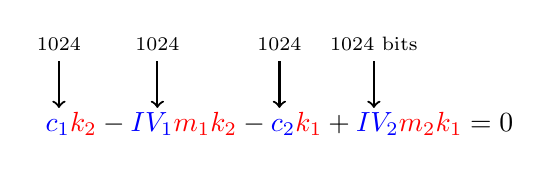
\begin{tikzpicture}[baseline=(eq.base)]
            \node (eq) at (0,0) {$\k{c_1}\u{k_2} - \k{IV_1}\u{m_1}\u{k_2} - \k{c_2}\u{k_1} +  \k{IV_2}\u{m_2}\u{k_1} =  0$};

            \foreach \x/\label in {
                -2.8/1024,
                -1.55/1024,
                 0./1024,
                 1.2/1024 bits
            } {
                \draw[<-, thick] (\x,0.2) -- ++(0,0.6) node[above] {\scriptsize \label};
            }
        \end{tikzpicture}
    \]

\pause

\begin{outline}
    \1 $0$ est engendré par $(\k{c_1})$, $(\k{IV_1})$, $(\k{c_2})$, $(\k{IV_2})$ 
        \pause
        \2[$\longrightarrow$]  LLL retourne bien $0$
    \1 Comment retrouver les coefficients utilisés?
    \pause
    \1 $\left[
    \begin{array}{ r c c c c}
        \k{c_1},  &1, &0, &0, &0  \\
        -\k{IV_1},&0, &1, &0, &0 \\
        -\k{c_2}, &0, &0, &1, &0 \\
        \k{IV_2}, &0, &0, &0, &1 \\
    \end{array}
    \right]$ engendre le vecteur $(0, \u{k_2},\u{m_1}\u{k_2},\u{k_1},\u{m_2}\u{k_1})$
    \pause
    \1 Il a pour taille (1, 256, 512, 256,512) bits. Est-il anormalement petit?
    \pause 
     \2[$\longrightarrow$] LLL trouve un vecteur de $(254, 251, 256, 255, 257)$ bits
\end{outline}
\end{frame} 

%------------------------------------------------
%------------------------------------------------



\begin{frame}{Changer la géométrie d'un réseau}

\begin{outline}
    \1 $\left[
    \begin{array}{r c c c c}
        \k{c_1} \times \mathbf{B},  &1, &0, &0, &0  \\
        -\k{IV_1} \times \mathbf{B}, &0, &1, &0, &0 \\
        -\k{c_2} \times \mathbf{B}, &0, &0, &1, &0 \\
        \k{IV_2} \times \mathbf{B}, &0, &0, &0, &1 \\
    \end{array}
    \right]$ engendre toujours $(0, \u{k_2},\u{m_1}\u{k_2},\u{k_1},\u{m_2}\u{k_1})$
    
    \pause \1 Un B gigantesque forcera la première composante à 0
        \2[$\longrightarrow$] LLL trouve un vecteur de taille $(1, 339, 339, 340, 341)$ bits
    \pause
    
    \vspace{0.5cm}
    
     \1 $\left[
    \begin{array}{r c c c c}
        \k{c_1} \times \mathbf{B},  &\mathbf{2^{256}}, &0, &0, &0  \\
        -\k{IV_1} \times \mathbf{B}, &0, &1, &0, &0 \\
        -\k{c_2} \times \mathbf{B}, &0, &0, &\mathbf{2^{256}}, &0 \\
        \k{IV_2} \times \mathbf{B}, &0, &0, &0, &1 \\
    \end{array}
    \right]$ engendre $(0, 2^{256}\u{k_2},\u{m_1}\u{k_2},2^{256}\u{k_1},\u{m_2}\u{k_1})$

        \pause
        
    \2[$\longrightarrow$] C'est bien le vecteur trouvé par LLL \flag{}
\end{outline}
\end{frame} 



% \begin{frame}{Sur les fonctions de hashage md5 et sha1}
    \large{\centerline{\textbf{Comment miner du bitcoin pour moins cher?}}}

\end{frame}

%------------------------------------------------
%------------------------------------------------

\begin{frame}{Fun with Hash \FiveStar\FiveStar \hfill 19 résolutions}
    \begin{columns}[c]
        \column{.45\textwidth}
        \begin{center}                  
            \includegraphics[width=0.9\textwidth]{img/meme/fun-intro.png}
        \end{center}

        \column{.65\textwidth} % 
           \begin{outline}
               \1 Objectifs : Générer un message $m$ tel que
                \2 $m$ commence par un challenge
                \2 $\text{sha1}(m)$ termine par les bytes 0xFC5C25
                \2 $\text{md5}(m)$ termine par les bytes 0xFC5C25
                \2 En moins de 30 minutes
           \end{outline}
    \end{columns}
\end{frame}

%------------------------------------------------
%------------------------------------------------

\begin{frame}{Comment générer des collisions}

    \vspace{-0.1cm}
    
   \begin{outline}
    \1 Brute force
        \2 Générer $m$ jusqu'à avoir les trois bytes de $md5(m)$ (une chance sur $2^{24}$)
        \pause
        \2 Prier pour les trois bytes de $sha1(m)$ (une chance sur $2^{24}$)
        \pause
        \2[$\longrightarrow$] Temps total O($2^{48}$)

    \pause
    
    \1 Pay2win
        \2 48 bits de collision nécessaire en 30 minutes $\longrightarrow$  155 GH/s (Giga hashs par seconde)
      \begin{table}
            \begin{tabular}{l l l}
                \toprule
                \textbf{Hardware} & \textbf{Hashs (GH/s)} & \textbf{Prix} \\
                \midrule
                NVIDIA GeForce RTX 4090   (SHA1)      & 52           & 2 174€              \\
                NVIDIA GeForce RTX 5090    (SHA1)     & 71           & 2 300€               \\
                FPGAs / ASIC (SHA1)        & 7.3   \footnote{\cite{6261737}} & 1 300€               \\
               % Le réseau bitcoin (SHA256) & 200 000 & 1 646 000 000€ \\
                \bottomrule
            \end{tabular}
            \caption{Quelques benchmarks de calcul de hashs, à la louche}
        \end{table}

        \vspace{-1.1cm}
        \pause 
        
        \1 Cryptanalyse
            \2 md5 : Collision en quelque secondes \cite{cryptoeprint:2006/104}
            
            \2 sha1 : Collision en quelques années GPUs \cite{10.5555/3489212.3489316}
   \end{outline}  
\end{frame}

%------------------------------------------------
%------------------------------------------------

\begin{frame}{Construction de Merkle-Damgård et collisions}
    \resizebox{18em}{!}{
        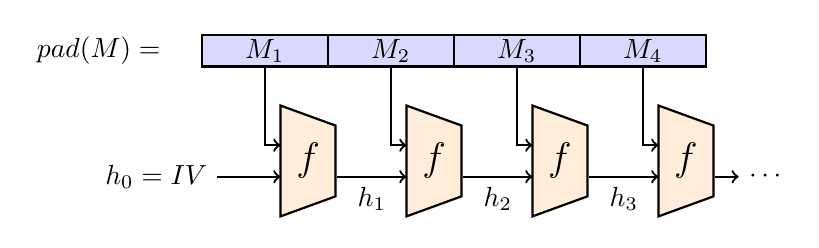
\begin{tikzpicture}[scale=0.4]
        \path[anchor=east] (-1,0.5) node {$pad(M)=$};
        \draw[fill=blue!15,thick,inner sep=2ex] (0,0) rectangle (16,1);
    
        %% Separations in the message
        \draw[thick] ++( 4,0) -- ++(0,1); \path (   2,0.5) node {$M_{1}$};
        \draw[thick] ++( 8,0) -- ++(0,1); \path ( 4+2,0.5) node {$M_{2}$};
        \draw[thick] ++(12,0) -- ++(0,1); \path ( 8+2,0.5) node {$M_{3}$};
        \draw[thick] ++(16,0) -- ++(0,1); \path (12+2,0.5) node {$M_{4}$};
    
        %% Compressions functions 
        \begin{scope}[shift={(0.5,-4)}]
            \node [draw,trapezium,trapezium left angle=70,trapezium right angle=70,minimum height=0.7cm,thick,fill=orange!15,shift={(1.15,0.4)},rotate=-90] 
            {\begin{sideways}\Large$f$\end{sideways}};
            \draw[->,thick] ++(1.5,+4) -- ++(0,-2.5) -- ++(0.5,0);
            \draw[->,thick] ++(0,0.5) node[left] {$h_{0}=IV$}-- ++(2,0);
        \end{scope}
    
        \begin{scope}[shift={(4.5,-4)}]
            \node [draw,trapezium,trapezium left angle=70,trapezium right angle=70,minimum height=0.7cm,thick,fill=orange!15,shift={(1.15,0.4)},rotate=-90] 
            {\begin{sideways}\Large$f$\end{sideways}};
            \draw[->,thick] ++(1.5,+4) -- ++(0,-2.5) -- ++(0.5,0);
            \draw[->,thick] ++(-0.2,0.5) -- node[below] {$h_{1}$} ++(2.2,0);
        \end{scope}
    
        \begin{scope}[shift={(8.5,-4)}]
            \node [draw,trapezium,trapezium left angle=70,trapezium right angle=70,minimum height=0.7cm,thick,fill=orange!15,shift={(1.15,0.4)},rotate=-90] 
            {\begin{sideways}\Large$f$\end{sideways}};
            \draw[->,thick] ++(1.5,+4) -- ++(0,-2.5) -- ++(0.5,0);
            \draw[->,thick] ++(-0.2,0.5) -- node[below] {$h_{2}$} ++(2.2,0);
        \end{scope}
    
        \begin{scope}[shift={(12.5,-4)}]
            \node [draw,trapezium,trapezium left angle=70,trapezium right angle=70,minimum height=0.7cm,thick,fill=orange!15,shift={(1.15,0.4)},rotate=-90] 
            {\begin{sideways}\Large$f$\end{sideways}};
            \draw[->,thick] ++(1.5,+4) -- ++(0,-2.5) -- ++(0.5,0);
            \draw[->,thick] ++(-0.2,0.5) -- node[below] {$h_{3}$} ++(2.2,0);
        \end{scope}
    
        \begin{scope}[shift={(16.5,-4)}]
            \draw[->,thick] ++(-0.2,0.5) -- ++(0.75,0) node[right] {$\cdots$} ;
        \end{scope}
    
    \end{tikzpicture}
    }
    \pause
    \resizebox{18em}{!}{
        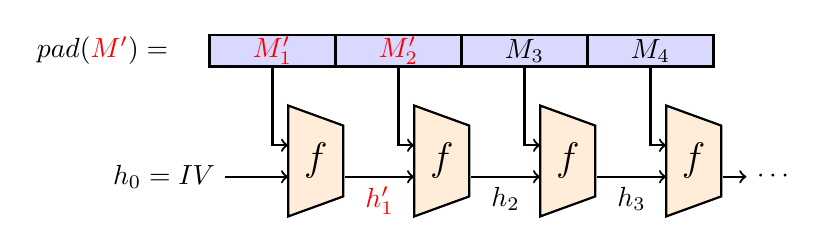
\begin{tikzpicture}[scale=0.4]
        	\path[anchor=east] (-1,0.5) node {$pad(\textcolor{red}{M'})=$};
        	\draw[fill=blue!15,thick,inner sep=2ex] (0,0) rectangle (16,1);
        
        	%% Separations in the message
        	\draw[thick] ++( 4,0) -- ++(0,1); \path (   2,0.5) node {$\textcolor{red}{M'_{1}}$};
        	\draw[thick] ++( 8,0) -- ++(0,1); \path ( 4+2,0.5) node {$\textcolor{red}{M'_{2}}$};
        	\draw[thick] ++(12,0) -- ++(0,1); \path ( 8+2,0.5) node {$M_{3}$};
        	\draw[thick] ++(16,0) -- ++(0,1); \path (12+2,0.5) node {$M_{4}$};
        
        	%% Compressions functions 
        	\begin{scope}[shift={(0.5,-4)}]
        		\node [draw,trapezium,trapezium left angle=70,trapezium right angle=70,minimum height=0.7cm,thick,fill=orange!15,shift={(1.15,0.4)},rotate=-90] 
        		{\begin{sideways}\Large$f$\end{sideways}};
        		\draw[->,thick] ++(1.5,+4) -- ++(0,-2.5) -- ++(0.5,0);
        		\draw[->,thick] ++(0,0.5) node[left] {$h_{0}=IV$}-- ++(2,0);
        	\end{scope}
        
        	\begin{scope}[shift={(4.5,-4)}]
        		\node [draw,trapezium,trapezium left angle=70,trapezium right angle=70,minimum height=0.7cm,thick,fill=orange!15,shift={(1.15,0.4)},rotate=-90] 
        		{\begin{sideways}\Large$f$\end{sideways}};
        		\draw[->,thick] ++(1.5,+4) -- ++(0,-2.5) -- ++(0.5,0);
        		\draw[->,thick] ++(-0.2,0.5) -- node[below] {$\textcolor{red}{h'_{1}}$} ++(2.2,0);
        	\end{scope}
        
        	\begin{scope}[shift={(8.5,-4)}]
        		\node [draw,trapezium,trapezium left angle=70,trapezium right angle=70,minimum height=0.7cm,thick,fill=orange!15,shift={(1.15,0.4)},rotate=-90] 
        		{\begin{sideways}\Large$f$\end{sideways}};
        		\draw[->,thick] ++(1.5,+4) -- ++(0,-2.5) -- ++(0.5,0);
        		\draw[->,thick] ++(-0.2,0.5) -- node[below] {$h_{2}$} ++(2.2,0);
        	\end{scope}
        
        	\begin{scope}[shift={(12.5,-4)}]
        		\node [draw,trapezium,trapezium left angle=70,trapezium right angle=70,minimum height=0.7cm,thick,fill=orange!15,shift={(1.15,0.4)},rotate=-90] 
        		{\begin{sideways}\Large$f$\end{sideways}};
        		\draw[->,thick] ++(1.5,+4) -- ++(0,-2.5) -- ++(0.5,0);
        		\draw[->,thick] ++(-0.2,0.5) -- node[below] {$h_{3}$} ++(2.2,0);
        	\end{scope}
        
        	\begin{scope}[shift={(16.5,-4)}]
        		\draw[->,thick] ++(-0.2,0.5) -- ++(0.75,0) node[right] {$\cdots$} ;
        	\end{scope}
            
        \end{tikzpicture}
    }
    \footnote{\cite{TikZ:for:Cryptographers}}
    \begin{outline}
        \1 Une collision pour $h_2$ entraînera une collision sur tous les états suivants
            \2[$\longrightarrow$] Si $md5(m)=md5(m')$, alors $md5(m||a) = md5(m'||a)$ 
        \pause
        \1 Dans notre cas :
            \2 Collision md5 pour $m$, $m'$ en quelques secondes \footnote{\url{https://github.com/cr-marcstevens/hashclash}}
            \pause
            \2 $2^{24}$ candidats $a$ pour pour avoir les 3 derniers bytes de $md5(m ||a)$ 
            \pause
            \2 On à gratuitement la même chose pour $md5(m' || a)$
            \pause
            \2 Ceci double les chances d'avoir une collision sur sha1
            \pause
            \2 Pourquoi s'arrêter là?
    \end{outline}
\end{frame}


%------------------------------------------------
%------------------------------------------------


\begin{frame}{Collisions multiples et md5}
\centering
    \resizebox{18em}{!}{
    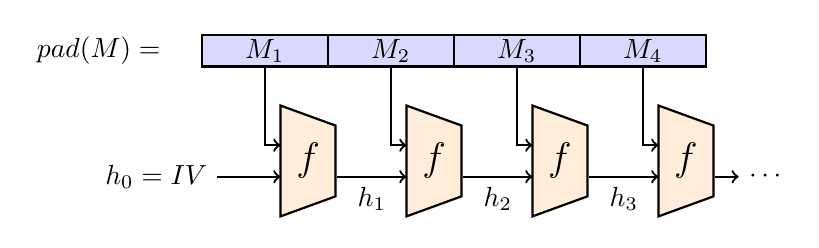
\begin{tikzpicture}[scale=0.4]
        \path[anchor=east] (-1,0.5) node {$pad(M)=$};
        \draw[fill=blue!15,thick,inner sep=2ex] (0,0) rectangle (16,1);
    
        %% Separations in the message
        \draw[thick] ++( 4,0) -- ++(0,1); \path (   2,0.5) node {$M_{1}$};
        \draw[thick] ++( 8,0) -- ++(0,1); \path ( 4+2,0.5) node {$M_{2}$};
        \draw[thick] ++(12,0) -- ++(0,1); \path ( 8+2,0.5) node {$M_{3}$};
        \draw[thick] ++(16,0) -- ++(0,1); \path (12+2,0.5) node {$M_{4}$};
    
        %% Compressions functions 
        \begin{scope}[shift={(0.5,-4)}]
            \node [draw,trapezium,trapezium left angle=70,trapezium right angle=70,minimum height=0.7cm,thick,fill=orange!15,shift={(1.15,0.4)},rotate=-90] 
            {\begin{sideways}\Large$f$\end{sideways}};
            \draw[->,thick] ++(1.5,+4) -- ++(0,-2.5) -- ++(0.5,0);
            \draw[->,thick] ++(0,0.5) node[left] {$h_{0}=IV$}-- ++(2,0);
        \end{scope}
    
        \begin{scope}[shift={(4.5,-4)}]
            \node [draw,trapezium,trapezium left angle=70,trapezium right angle=70,minimum height=0.7cm,thick,fill=orange!15,shift={(1.15,0.4)},rotate=-90] 
            {\begin{sideways}\Large$f$\end{sideways}};
            \draw[->,thick] ++(1.5,+4) -- ++(0,-2.5) -- ++(0.5,0);
            \draw[->,thick] ++(-0.2,0.5) -- node[below] {$h_{1}$} ++(2.2,0);
        \end{scope}
    
        \begin{scope}[shift={(8.5,-4)}]
            \node [draw,trapezium,trapezium left angle=70,trapezium right angle=70,minimum height=0.7cm,thick,fill=orange!15,shift={(1.15,0.4)},rotate=-90] 
            {\begin{sideways}\Large$f$\end{sideways}};
            \draw[->,thick] ++(1.5,+4) -- ++(0,-2.5) -- ++(0.5,0);
            \draw[->,thick] ++(-0.2,0.5) -- node[below] {$h_{2}$} ++(2.2,0);
        \end{scope}
    
        \begin{scope}[shift={(12.5,-4)}]
            \node [draw,trapezium,trapezium left angle=70,trapezium right angle=70,minimum height=0.7cm,thick,fill=orange!15,shift={(1.15,0.4)},rotate=-90] 
            {\begin{sideways}\Large$f$\end{sideways}};
            \draw[->,thick] ++(1.5,+4) -- ++(0,-2.5) -- ++(0.5,0);
            \draw[->,thick] ++(-0.2,0.5) -- node[below] {$h_{3}$} ++(2.2,0);
        \end{scope}
    
        \begin{scope}[shift={(16.5,-4)}]
            \draw[->,thick] ++(-0.2,0.5) -- ++(0.75,0) node[right] {$\cdots$} ;
        \end{scope}
    \end{tikzpicture}
    }

    \pause
    
    \begin{itemize}
        \item Pour IV fixé, trouver $m_1$ et $m'_1$ en collision sur $h_1$
        \pause
        \item Pour $h_1$ trouver $m_2$ et $m'_2$ en collision sur $h_2$
        \pause
        \item etc
    \end{itemize}
    \pause
    \resizebox{25em}{!}{
        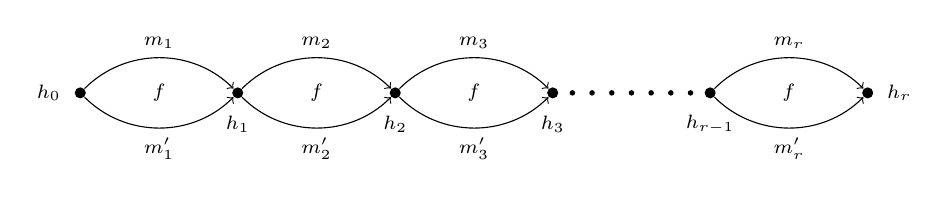
\begin{tikzpicture}[scale=1]
        
           \draw (0,0) node[fill,circle,inner sep=0pt,minimum size=4pt] (a1) {};%
           \draw (2,0) node[fill,circle,inner sep=0pt,minimum size=4pt] (a2) {};%
           \draw (4,0) node[fill,circle,inner sep=0pt,minimum size=4pt] (a3) {};%
           \draw (6,0) node[fill,circle,inner sep=0pt,minimum size=4pt] (a4) {};%
        
           \draw (6.25,0) node[fill,circle,inner sep=0pt,minimum size=2pt] (b0) {};%
           \draw (6.5,0) node[fill,circle,inner sep=0pt,minimum size=2pt] (b1) {};%
           \draw (6.75,0) node[fill,circle,inner sep=0pt,minimum size=2pt] (b2) {};%
           \draw (7,0) node[fill,circle,inner sep=0pt,minimum size=2pt] (b3) {};%
           \draw (7.25,0) node[fill,circle,inner sep=0pt,minimum size=2pt] (b4) {};%
           \draw (7.5,0) node[fill,circle,inner sep=0pt,minimum size=2pt] (b5) {};%
           \draw (7.75,0) node[fill,circle,inner sep=0pt,minimum size=2pt] (b6) {};%
        
           \draw (8,0) node[fill,circle,inner sep=0pt,minimum size=4pt] (a5) {};%
           \draw (10,0) node[fill,circle,inner sep=0pt,minimum size=4pt] (a6) {};%
          
           \draw[->] (a1) edge[out= 45, in= 3*45] node[above]{\scriptsize $m_{1}$} (a2);
           \draw[->] (a1) edge[out=-45, in=-3*45] node[below]{\scriptsize $m'_{1}$} (a2);
          
           \draw[->] (a2) edge[out= 45, in= 3*45] node[above]{\scriptsize $m_{2}$} (a3);
           \draw[->] (a2) edge[out=-45, in=-3*45] node[below]{\scriptsize $m'_{2}$} (a3);
          
           \draw[->] (a3) edge[out= 45, in= 3*45] node[above]{\scriptsize $m_{3}$} (a4);
           \draw[->] (a3) edge[out=-45, in=-3*45] node[below]{\scriptsize $m'_{3}$} (a4);
           
           \draw[->] (a5) edge[out= 45, in= 3*45] node[above]{\scriptsize $m_{r}$} (a6);
           \draw[->] (a5) edge[out=-45, in=-3*45] node[below]{\scriptsize $m'_{r}$} (a6);
           
           \path (1,0) node {\scriptsize $f$};
           \path (3,0) node {\scriptsize $f$};
           \path (5,0) node {\scriptsize $f$};
           \path (9,0) node {\scriptsize $f$};
           
          
           \path (-0.4,0) node {\scriptsize $h_{0}$};
           \path (2,-0.4) node {\scriptsize $h_{1}$};
           \path (4,-0.4) node {\scriptsize $h_{2}$};
           \path (6,-0.4) node {\scriptsize $h_{3}$};
           \path (8,-0.4) node {\scriptsize $h_{r-1}$};
           \path (10+0.4,0) node {\scriptsize $h_{r}$};
        
        \end{tikzpicture}
    }
    \begin{outline}
        \1 $2^{r}$ collisions sur $h_r$ générées pour le prix de $r$
        \pause
        \1 Dans notre cas
            \2 On génère facilement $2^{24}$ collisions $md5(x_1)= \cdots = md5(x_{2^{24}})$
            \pause
            \2 On itère sur $2^{24}$ valeurs de $a$ jusqu'à avoir la collision sur $md5(x_1 || a)$
            \pause
            \2 Statistiquement, il y a une collision pour au moins un des $sha1(x_i || a)$  $\flag$
    \end{outline}
\end{frame}

% \begin{frame}{Kyber et les anneaux quotients}
    \large{\centerline{\textbf{}}}

\end{frame}

%------------------------------------------------
%------------------------------------------------

\begin{frame}{Kzber \FiveStar \FiveStar\FiveStar \hfill 25 résolutions}
    \begin{columns}[c]
        \column{.45\textwidth}
        \begin{center}                  
            \includegraphics[width=0.9\textwidth]{img/meme/kyber-intro.png}
        \end{center}

        \column{.65\textwidth} % 
           \begin{outline}
                \1 Objectifs : 
                    \2 Récupérer $\u{k}$ sur 128 bits  chiffré via Kyber
                \1 Données :
                    \2 La clef publique $\k{A}$ et $\k{t}$
                    \2 Le chiffré $E(\u{k})$
                    \2 Le code source
           \end{outline}
    \end{columns}
\end{frame}

%------------------------------------------------
%------------------------------------------------

\begin{frame}{Kyber / ML-KEM (le vrai)}
PQ-KEM (chiffrement asymétrique) standardisé par le NIST
\pause
   \begin{block}{\only<3->{Ring/Module }Learning with Errors (\only<3->{R/M}LwE)}
   Soit $\k{A}\in\mathbb{Z}_q^{k\times k}$.
       \begin{itemize}
        \item Facile de récupérer $\u{s}\in\mathbb{Z}_q^k$ sachant $\k{t}=\k{A}.\u{s}$ (Interpolation)
        \pause
        \item Difficile  de récupérer $\u{s}\in\mathbb{Z}_q^k$ sachant $\k{t}=\k{A}.\u{s}+\u{e}$ où $\u{e}\in\mathbb{Z}_q^{k}$ est petit ($|\u{e}|<\eta$)
        \pause 
        \item Même chose dans $\mathcal{R}_q^k = \left(\mathbb{Z}_q[X]/\left<\phi\right>\right)^k$, et $\phi$ de degré $n$
       \end{itemize}
   \end{block}
   \pause
   \begin{table}
        \begin{tabular}{c|c|c|c|c}
            Nom       & n   & k & q    & $\eta$ \\
            \hline
            Kyber512  & 256 & 2 & 3329 & 2\\
            Kyber768  & 256 & 3 & 3329 & 2\\
            Kyber1024 & 256 & 4 & 3329 & 2\\
        \end{tabular}
    \end{table}
    \pause 
    $\mathcal{R}_q = \mathbb{Z}_q[X]/(X^n+1)$
\end{frame}

\begin{frame}{Algorithmes de Kyber}
    \begin{columns}[c]
        \column{.5\textwidth}
            \begin{outline}
                \1 \textbf{Keygen} : $\k{t} = \k{A}. \u{s}+\u{e}$ 
                    \2 Clef privée $(\u{s})$
                    \2 Clef publique $(\k{A},\k{t})$
                \pause
                \1 \textbf{Chiffrement $m$} : 
                    \2 $\left\{
                \begin{array}{c c l}
                   \k{u} & = & \k{A}^T\u{r} + \u{e_1}\\
                   \k{v} & = & \k{t}^T\u{r}+\u{e_2} + m\\
                \end{array}
                \right.$
                \pause
                \1 \textbf{Déchiffrement $(u,v)$} : 
                    \2 $\k{v}-\u{s}^T\k{u} = m +\u{e}^T\u{r}+\u{e_2} + \u{s}^T\u{e_1} = m + \u{e_3}$
                \end{outline}
        \column{.65\textwidth} % 
        \begin{center}   
            \only<4>{
                \includegraphics[width=0.8\textwidth]{img/crypto/kyber/kyber-modulo.png}
            }
            \only<5>{
                \includegraphics[width=0.8\textwidth]{img/crypto/kyber/kyber-chose_m.png}
            }
            \only<6>{
                \includegraphics[width=0.8\textwidth]{img/crypto/kyber/kyber-1 or 0.png}
            }
            \only<7>{
                \includegraphics[width=0.8\textwidth]{img/crypto/kyber/kyber-add error.png}
            }
            \only<8->{
                \includegraphics[width=0.8\textwidth]{img/crypto/kyber/kyber-decrypt.png}
            }
        \end{center}
   \end{columns}
   \pause
   $m$ est un polynôme de $\mathcal{R}_q$ (e.g $0101$ devient $0+\frac{q}{2}x+0x^2+\frac{q}{2}x^3$)
\end{frame}

\begin{frame}{Retour au challenge : La (les?) typos}
    \begin{outline}
        \1 $E(m_0),\dots,E(m_k)$ au lieu de $E(m_0,\dots,m_k)$
            \2 $m$ est le polynôme constant 0 ou $q/2$

        \vspace{0.2cm}
        \pause
        
        \1 Travail modulo $X^n\textbf{-}1$ (au lieu de $X^n+1$) qui admet des racines dans $\mathbb{Z}_q$ 
        \pause
            \2 $P\mapsto P(1)$ est un morphisme d'anneau sur $\mathcal{R}_q$ % $\longrightarrow$ somme des coefficients
	    	\3 C'est le morphisme $P \mapsto P \mod X-1$

            \vspace{0.1cm}
            \pause
            
            \2  $\k{v}(1) = \left[\k{t_0}(1),\,\k{t_1}(1)\right]\bullet \left[\u{r_0}(1),\,\u{r_1}(1)\right]^{T}+\u{e_2}(1) + m(1)$ \pause $\in[-q/2,q/2]$ 
            \pause
                \3 $\k{v}(1) = \k{0}+\u{e_2}(1) + m$  avec probabilité $1/q^2$ \hfill ($\sim\frac{1}{11\,082\,241}$)
                \pause
                \3 $\k{v}(1) = \k{\epsilon}\u{r_0}(1)+\k{\epsilon}\u{r_1}(1)+\u{e_2}(1) + m$  avec probabilité $\epsilon^2/q^2$ \hfill ($\sim\frac{1}{12\,313}$)
                \pause
                %\3 Bruteforce des valeurs de $\u{r_0}(1),\u{r_1}(1)$ (à réinjecter dans $\k{v}=\k{A}\cdot\u{r}+\u{e_2}$)

            \vspace{0.1cm}
            \pause
            
            \2 $P\mapsto P(-1)$ est aussi un morphisme d'anneau \hfill ($\sim\frac{1}{6\,156}$)
	    	\3 C'est le morphisme $P \mapsto P \mod X+1$

            \vspace{0.1cm}
            \pause
            
            \2 $X^{256}-1$ à exactement 256 racines dans $\mathbb{Z}_q$ (et $X^{256}+1$ n'en a pas)
		\3 Difficile à exploiter car $\u{e_2}(r)$ est grand
		
		\pause
	    \2 $X^{256}-1$ est divisible par $X^{2^k}-1$  (et $X^{256}+1$ n'en a pas)\hfill ($\sim\frac{1}{96}$)
        \vspace{0.2cm}
        \pause

        \1 On peut générer des instances du problème jusqu'à avoir la solution via au moins l'un de ces morphismes $\flag$

    \end{outline}
\end{frame}

% \begin{frame}{Analyse différentielle et boomerang}
    \large{\centerline{\textbf{Attaque sur SbPN}}}

\end{frame}

%------------------------------------------------
%------------------------------------------------

\begin{frame}{Le retour de Jafar \FiveStar \FiveStar \hfill \textcolor{red}{8 résolutions :(}}
    \begin{columns}[c]
        \column{.45\textwidth}
        \begin{center}                  
            \includegraphics[width=0.9\textwidth]{img/meme/jafar-intro.png}
        \end{center}

        \column{.65\textwidth} % 
           \begin{outline}
                \1 Objectifs : 
                    \2 Forger un couple clair / chiffré sans connaître la clef

                    \pause 
                \1 Données
                    \2 Exactement 3 oracles de chiffrement / déchiffrement
                    \2 Le code source
           \end{outline}
    \end{columns}
\end{frame}


%------------------------------------------------
%------------------------------------------------

\begin{frame}{Le cipher Jafar}
  \begin{columns}[c]
        \column{.50\textwidth} %
             \begin{center}                  
                \includegraphics[width=0.9\textwidth]{img/crypto/jafar/jafar-scheme.png}
            \end{center}
        \column{.50\textwidth}
           \begin{outline}
                \1 40 tours au total
                \pause
                \1 Pas de tour de clef
                \pause
                \1 Tout est linéaire à part la SBox
                \pause
                \begin{center}                  
                 \includegraphics[width=0.9\textwidth]{img/meme/jafar-meme.png}
                \end{center}
                \hfill \tiny{@bluesheet}
           \end{outline}
    \end{columns}
\end{frame}

%------------------------------------------------
%------------------------------------------------

\begin{frame}[fragile] % <---
\frametitle{Fausse piste : la permutation}
  \begin{columns}[c]

    \column{.45\textwidth}
        \begin{lstlisting}[language=Python]
P_Perm = Permutation(P)
P_perm.show("braid")
P_perm.fixed_points()
P_perm.cycle_tuples()
        \end{lstlisting}

        \begin{itemize}
            \item Deux points fixes (2 et 94)
            \item Trois cycles non triviaux de taille 82, 31, 13
        \end{itemize}
    \column{.40\textwidth} %
        \begin{center}                  
            \includegraphics[width=0.9\textwidth]{img/crypto/jafar/permutation.png}
        \end{center}
    \end{columns}

\end{frame}


\begin{frame}[fragile] % <---
\frametitle{Analyse de la SBox}
  \begin{columns}[c]
    \column{.70\textwidth}
        \begin{lstlisting}[language=Python]
from sage.crypto.sbox import SBox
sb = SBox(S)
sb.difference_distribution_table()
\end{lstlisting}
        \begin{outline}
            \1 DDT[a,b] := Probabilité que $S[x\oplus a] = S[x]\oplus b$
            
            \only<2->{
                \2[$\longrightarrow$] 4 différentielles par Sbox: $(0\mapsto 0)$ ,$(24\mapsto 129)$, $(74\mapsto 7)$, $(82 \mapsto 134)$
                }
            \only<3->{
            \1 16 octets $\Rightarrow$ $2^{32}$ différentielles à tester
            }
        \end{outline}
    \column{.30\textwidth} %
        \begin{center}                  
            \includegraphics[trim=30pt 140pt 30pt 140pt, clip, width=0.9\textwidth]{img/crypto/jafar/AES-ddt.png}
        \end{center}
        \pause 
        \begin{center}                  
            \includegraphics[trim=30pt 30pt 30pt 100pt, clip, width=0.9\textwidth]{img/crypto/jafar/sbox-ddt.png}
        \end{center}
    \end{columns}

\end{frame}



\begin{frame}{Introduire une différentielle}
        \begin{center}                  
            \includegraphics[width=0.53\textwidth]{img/crypto/jafar/auto/1round.png}
        \end{center}
        \pause
    \begin{itemize}
        \item $D_{in}=[0, 82, 0, 24, 0, 0, 0, 82, 0, 0, 0, 0, 0, 0, 0, 0]$
        \item $D_{out}=[0, 0, 0, 0, 0, 74, 0, 0, 0, 0, 24, 0, 0, 74, 0, 0]$
    \end{itemize}

\end{frame}


\begin{frame}{Sur 20 rounds}
        \begin{center}                  
            \includegraphics[width=0.6\textwidth]{img/crypto/jafar/auto/first-try.png}
        \end{center}
\end{frame}

\begin{frame}{Introduction au boomerang \only<6>{\flag}}
    \only<1>{
        \begin{center}                  
            \includegraphics[scale=0.5]{img/crypto/jafar/auto/boomerang-1.png}
        \end{center}
    }
    \only<2>{
        \begin{center}                  
            \includegraphics[scale=0.5]{img/crypto/jafar/auto/boomerang-2.png}
        \end{center}
    }
    \only<3>{
        \begin{center}                  
            \includegraphics[scale=0.5]{img/crypto/jafar/auto/boomerang-3.png}
        \end{center}
    }
    \only<4>{
        \begin{center}                  
            \includegraphics[scale=0.5]{img/crypto/jafar/auto/boomerang-4.png}
        \end{center}
    }
    \only<5->{
        \begin{center}                  
            \includegraphics[scale=0.5]{img/crypto/jafar/auto/boomerang-5.png}
        \end{center}
    }

\end{frame}
% \begin{frame}{Le schéma multivarié UOV}
    \large{\centerline{\textbf{Comment faire une (mauvaise) vinaigrette}}}
     \centering
    \includegraphics[trim=12cm 8cm 8cm 8cm, clip, width=0.5\linewidth]{img/meme/UOV-vac.jpg}
\end{frame}

%------------------------------------------------
%------------------------------------------------

\begin{frame}{Ça tourne au vinaigre \FiveStar\FiveStar\FiveStar \hfill 9 résolutions}
    \begin{columns}[c]
        \column{.55\textwidth}
        \begin{center}                  
            \includegraphics[width=0.9\textwidth]{img/meme/uov-intro.png}
        \end{center}

        \column{.45\textwidth} % 
           \begin{outline}
               \1 Objectifs :
                \2 Forger une signature valide
                \2 Sans la clef privée
                \pause
                \2 \textcolor{red}{Sans la clef publique}
                \pause
               \1 Données :
                    \2 1600 signatures

           \end{outline}
    \end{columns}
\end{frame}

%------------------------------------------------
%------------------------------------------------

%------------------------------------------------
%------------------------------------------------

\begin{frame}{Sur les représentations des fonctions quadratiques}
    \begin{columns}[c]
        \column{.50\textwidth}

            \begin{block}{Fonction quadratique}
                $f(x_1,\dots,x_n) = $
                \only<1>{
                    $\underset{i\leq j}{\displaystyle\sum} a_{ij}x_ix_j$ 
                }
                \only<2->{
                    \colorbox{blue!20}{$\underset{i\leq j}{\displaystyle\sum}a_{ij}x_ix_j$}
                }
                $ + $
                \only<1>{
                    $\underset{i}{\displaystyle\sum} b_{i}x_i$
                }
                \only<2->{
                    \colorbox{red!20}{$\underset{i}{\displaystyle\sum} b_{i}x_i$}
                }
                $ +\, c$
                \only<2->{
                    \\
                    \hspace{2.55cm}
                        \text{\scriptsize\color{blue!60} (quadratique)}
                    \hspace{0.65cm}
                        \text{\scriptsize\color{red!60} (linéaire)}
                }
            \end{block}
            \pause
            \begin{block}{Forme quadratique}             
                $f'(\textbf{x},\textbf{x}) = \underset{i\leq j}{\displaystyle\sum} a_{ij}x_i x_j$ \pause $= \textbf{x}^T \textbf{A} \textbf{x}$
            \end{block}

        \column{.45\textwidth}
            \only<3>{
            \begin{figure}
                \centering
                \includegraphics[width=5cm]{img/crypto/UOV/quadratic.png}
                \begin{tikzpicture}[overlay, remember picture]
                \end{tikzpicture}
                \captionsetup{labelformat=empty} % Removes the 'Figure' label
                \caption{Représentation matricielle d'une forme quadratique}

            \end{figure}
            }
            \only<4->{
                \begin{figure}
                \begin{tikzpicture}
                
                    \node[anchor=south west,inner sep=0] (image) at (0,0) {\includegraphics[width=5cm]{img/crypto/UOV/quadratic.png}};
                    \begin{scope}[x={(image.south east)}, y={(image.north west)}]
                        % Adjust these coordinates (0–1 range) to point to your (i,j) coefficient
                        \def\x{0.7}
                        \def\y{0.6}
                        \def\size{0.01}
                
                        % Draw square around pixel
                        \draw[red, line width=1.5mm] (\x-\size, \y-\size) rectangle (\x+\size, \y+\size);
                
                        % Axis labels
                        \node[above=2pt, xshift=\x*5cm, text=red] at (image.north west) {$j$};
                        \node[right=2pt, yshift=\y*5cm, text=red] at (image.south east) {$i$};
                            \node[red, right=\x*2.5cm, yshift=\y*2.5cm] {$a_{ij}x_ix_j$};
                    \end{scope}
            \end{tikzpicture}
            \captionsetup{labelformat=empty} % Removes the 'Figure' label
            \caption{Représentation matricielle d'une forme quadratique}
            \end{figure}
        }
    \end{columns}

\end{frame}

\begin{frame}{Sur les formes bilinéaires}

$f(x_1,\dots,x_n) = \underset{i\leq j}{\displaystyle\sum} a_{ij}x_ix_j + \underset{i}{\displaystyle\sum} b_{i}x_i + c$
    \begin{block}{Forme bilinéaire}             
        $f'(\textbf{x},\textbf{y}) = \underset{i\leq j}{\displaystyle\sum} a_{ij}x_i y_j$ \pause $= \textbf{x}^T \textbf{G} \textbf{y}$ \pause \hfill $/!\backslash$ $\textbf{}G$ est de taille maximale
    \end{block}
    \pause
    \begin{itemize}
        \item Pour $\textbf{y}$ fixé, une équation en $\textbf{x}$ est linéaire (et vice versa)
    \end{itemize}
    \pause
    \begin{block}{Composition}
        $f'(\textbf{x},\textbf{y})=f(\textbf{x}+\textbf{y})-f(\textbf{x}) - f(\textbf{y})+f(\textbf{0})$ est une forme bilinéaire symétrique
    \end{block}

    \begin{itemize}
      \item  Les parties linéaires et constantes se simplifient
      \item $(\textbf{x}+\textbf{y})^T \textbf{A}(\textbf{x}+\textbf{y}) = \textbf{x}^T\textbf{A}\textbf{x}+\textbf{y}^T\textbf{A}\textbf{y}+\textbf{x}^T(\textbf{A}+\textbf{A}^T)\textbf{y}$
    \end{itemize}
    
\end{frame}

\begin{frame}{Une signature via UOV (Unbalanced Oil and Vinegar)}
    
    \begin{block}{La clef publique UOV}
        $\mathcal{Q}=(\mathcal{Q}_1,\dots,\mathcal{Q}_h)$ des fonctions quadratiques à n variables

        $\mathcal{Q}_i(\textbf{y}) = \textbf{y}^T\textbf{A}_i\textbf{y} + \textbf{b}_i^T\textbf{y} + c_i $
    \end{block}
    \pause
    La signature de $\textbf{t}=(t_1,\dots,t_h)$ est une solution $\textbf{y}=(y_1,\dots,y_n)$ du système $\mathcal{Q}(\textbf{y})=\textbf{t}$ :
    \[\left\{
    \begin{array}{c}
       \mathcal{Q}_1(\textbf{y}) =  \mathcal{Q}_1(y_1,\dots,y_n) = t_1 \\
       \vdots \\
       \mathcal{Q}_h(\textbf{y}) =  \mathcal{Q}_h(y_1,\dots,y_n) = t_h \\
    \end{array}
    \right.\]
    \pause
    \begin{block}{Difficulté du problème UOV}
        Pour des bonnes valeurs de $h$, $v$ et $n=h+v$ , il est difficile de résoudre un tel système quadratique quelconque.
    \end{block}
    \pause
    Sans clef privée, il est difficile de signer un message
\end{frame}

\begin{frame}{La trapdoor d'UOV}
$\mathbb{F}_q^n=\mathbb{F}_q^h \oplus\mathbb{F}_q^v = \mathcal{H}\oplus\mathcal{V}$ (huile + vinaigre) $\pause \Rightarrow$ $\textbf{x} =(x_1,\dots,x_h,x_{h+1},\dots,x_{h+v}) = (\mathbf{x}_\mathcal{H},\mathbf{x}_\mathcal{V})$
    \pause
    \begin{columns}
        \column{.45\textwidth}
            \begin{figure}
                \begin{tikzpicture}
                
                    \node[anchor=south west,inner sep=0] (image) at (0,0) {\includegraphics[width=3cm]{img/crypto/UOV/quadratic.png}};
                    \begin{scope}[x={(image.south east)}, y={(image.north west)}]
                        % Adjust these coordinates (0–1 range) to point to your (i,j) coefficient
                        \def\x{0.7}
                        \def\y{0.6}
                        \def\size{0.01}
                
                        % Draw square around pixel
                        \draw[red, line width=1.5mm] (\x-\size, \y-\size) rectangle (\x+\size, \y+\size);
                
                        % Axis labels
                        \node[above=2pt, xshift=\x*3cm, text=red] at (image.north west) {$j$};
                        \node[right=2pt, yshift=\y*3cm, text=red] at (image.south east) {$i$};
                            \node[red, right=\x*1cm, yshift=\y*1cm] {$a_{ij}y_iy_j$};
                    \end{scope}
            \end{tikzpicture}
            \captionsetup{labelformat=empty} % Removes the 'Figure' label
            \caption{Partie quadratique de $\mathcal{Q}_i$ publique}
            \end{figure}
        \pause
        \column{.05\textwidth}
        $\overset{\mathbf{y}=\mathcal{S}(\mathbf{x})}{\Leftarrow}$
        \column{.45\textwidth}
            \begin{figure}
                \begin{tikzpicture}
                
                    \node[anchor=south west,inner sep=0] (image) at (0,0) {\includegraphics[width=3cm]{img/crypto/UOV/trapdoor.png}};
                    \begin{scope}[x={(image.south east)}, y={(image.north west)}]
                        % Adjust these coordinates (0–1 range) to point to your (i,j) coefficient
                        \def\x{0.25}
                        \def\y{0.8}
                        \def\size{0.2}

                        \only<5->{
                            % Draw square around pixel
                            \draw[red, line width=1.5mm] (\x-\size, \y-\size) rectangle (\x+\size, \y+\size);
                    
                            % Axis labels
                            \node[red, right=\x*0cm, yshift=\y*1cm] {\shortstack{$a'_{ij}=0$ \\ pour $i,j<h$}};
                        }
                    \end{scope}
            \end{tikzpicture}
            \captionsetup{labelformat=empty} % Removes the 'Figure' label
            \caption{Partie quadratique de $\mathcal{P}_i=\mathcal{Q}_i\circ \mathcal{S}$ privée}
            \end{figure}
    \end{columns}
    \pause
    \begin{itemize}
        \item Par construction, $\mathcal{P}_i(\mathbf{x})=\mathcal{P}_i((\mathbf{x}_\mathcal{H},\mathbf{x}_\mathcal{V}))$ est \textit{linéaire} en $\mathbf{x}_\mathcal{H}$ pour $\mathbf{x}_\mathcal{V}$ fixé.
        \pause
        \item Pour $\mathbf{x}_\mathcal{V}$ fixé, il est trivial de résoudre $\mathcal{P}(\mathbf{x}_\mathcal{H},\mathbf{x}_\mathcal{V})=\mathbf{t}$
        \pause
        \item Pour $\mathbf{y}=\mathcal{S}(\mathbf{x})$ sera une solution valide de $\mathcal{Q}(\mathbf{y}) =\mathbf{t}$
    \end{itemize}
    
\end{frame}

\begin{frame}{Récapitulatif d'UOV}
    \pause
    \begin{block}{Keygen}
        \begin{itemize}
            \item Générer un changement de variable linéaire $\mathcal{S}$ aléatoire (matrice $n\times n$)
            \pause
            \item Générer $\mathcal{P}_{i<h}$ quadratique tels que $\mathcal{P}_i((\mathbf{x}_\mathcal{H},\mathbf{x}_\mathcal{V}))$ est linéaire en $\mathbf{x}_\mathcal{H}$ pour $\mathbf{x}_\mathcal{V}$ fixé
            \pause
            \item \textbf{Clef publique} : $\mathcal{Q} = \mathcal{P}\circ \mathcal{S}^{-1}$ avec  $h{{n+1}\choose{2}}$ coefficients 
            \pause
            \item \textbf{Clef privée} : $\mathcal{P}$, $\mathcal{S}$ avec $h\left({{n+1}\choose{2}}-{{h}\choose{2}}\right)$ et $n^2$ coefficients 
        \end{itemize}
    \end{block}

    \pause
    \begin{block}{Signature de $m$}
        \begin{itemize}
            \pause
            \item Encoder $m$ comme $\mathbf{t}\in\mathbb{F}_q^h$
            \pause
            \item Fixer aléatoirement $\mathbf{x}_\mathcal{V}\in\mathcal{V}$
            \pause
            \item Résoudre $\mathcal{P}((\mathbf{x}_\mathcal{H},\mathbf{x}_\mathcal{V}))=\mathbf{t}$ (linéaire en $\mathbf{x}_\mathcal{H}$). Si pas de solution, choisir un autre $\mathbf{x}_\mathcal{V}$
            \pause
            \item \textbf{Signature}: $\mathbf{y} = \mathcal{S}(\mathbf{x})$ est une solution du système $\mathcal{Q}(\mathbf{y}) =\mathbf{t}$
        \end{itemize}
    \end{block}
\end{frame}

\begin{frame}{Retour au challenge}
    \begin{block}{Parametres}
        \begin{itemize}
            \item $n=60$, donc polynômes à 60 variables, vecteurs $\mathbf{x}$, $\mathbf{y}$ de dimensions 60 
            \item $h=24$, donc 24 équations quadratiques $\mathcal{P}_i$ et $\mathcal{Q}_i$
            \item $v=n-h=36$, donc 36 variables de $\mathbf{x}_\mathcal{V}$ à fixer pour la signature
        \end{itemize}
    \end{block}

\pause
\vspace{0.6cm}

    \begin{outline}
        \1 Analyse du code source
    \end{outline}

            \begin{columns}
                \column{.45\textwidth}
                \begin{tcolorbox}
                    \begin{minipage}{\columnwidth}
    \textbf{Keygen}: La clef privée inverse $h$ et $v$ (au lieu d'avoir 24 inconnues linéaires dans la clef privée, on en a 36)
                    \end{minipage}%
                \end{tcolorbox}
                \pause
                \column{.45\textwidth}

                \begin{tcolorbox}
                    \begin{minipage}{\columnwidth}
    \textbf{Signature}: les 36 valeurs de $\mathbf{x}_\mathcal{V}$ sont déterministes, calculées via SHAKE256 du message, donc connues
                    \end{minipage}%
                \end{tcolorbox}

            \end{columns}       
\end{frame}

\newcommand{\vin}{\mathcal{V}}
\newcommand{\hui}{\mathcal{H}}
\renewcommand{\S}{{\mathcal{S}}}
\newcommand{\sV}{{\mathcal{S}_{|\vin}}}
\newcommand{\sH}{{\mathcal{S}_{|\hui}}}

\newcommand{\xV}{\mathbf{x}_\vin}
\newcommand{\xH}{\mathbf{x}_\hui}
\newcommand{\yV}{\mathbf{y}_{\vin'}}
\newcommand{\yH}{\mathbf{y}_{\hui'}}



\begin{frame}{Sur la confidentialité des vecteurs vinaigres \footnote{\cite{cryptoeprint:2023/1131}}}

    \pause 

    $\mathbf{\k{y}}=\S(\mathbf{\u{x}})=\S(\k{\xV})+\S(\u{\xH})=\sV(\k{\xV})+\sH(\u{\xH})$ car $\mathbb{F}_q^n =\vin\oplus \hui$ 

    Avec $\sV:\vin\longrightarrow \S(\vin):=\vin'$ et $\sH:\hui\longrightarrow \S(\hui):=\hui'$ des \textit{isomorphismes}
    
    \vspace{0.4cm}
    \pause 
    
       Ceci donne $\sV^{*}(\mathbf{\k{y}}) = \mathbf{\k{x_\vin}} + 0$ \pause $\longrightarrow$ On interpole $\sV$ donc $\vin'$ avec $36*60/36=60$ signatures

    \vspace{0.4cm}
    \pause
    Comme $\mathcal{P}$ est linéaire sur $\hui$, après changement de variable $\mathcal{Q}=\mathcal{P}\circ \S$ sera linéaire sur $\hui'$

    \begin{block}{Forger une signature UOV}
         $\mathbb{F}_q^n =\vin' + \hui'$, donc connaître l'espace $\vin'$ ou $\hui'$ suffit à forger une signature UOV
    \end{block}

%    Ainsi $\hui'\bigcap\vin' = \{0\}$ et donc $\sV^{-1}\circ\sH = 0$

    \vfill
   \pause

   On a toujours pas la clef publique...
\end{frame}

\begin{frame}{Récupérer la clef publique}
On a 1600 signatures :
    \begin{outline}
        
        \1 Interpolation polynomiale de la clef publique $\u{\mathcal{Q}_i}: \k{\mathbf{y}} \mapsto \k{\mathbf{t}_i}$ 
            \2 ${{n+1}\choose{2}}=1891$ inconnues pour chaque $\u{\mathcal{Q}_i}$ \pause $\rightarrow$ n'exploite par la connaissance de $\vin'$

        \pause
        
        \1 Interpolation polynomiale de la clef privée, $\u{\mathcal{P}_i} : \k{\xV} \oplus \u{\xH} \mapsto \k{\mathbf{t_i}}$
            \2 $\left({{n+1}\choose{2}}-{{h}\choose{2}}\right)=1591$ inconnues par $\u{\mathcal{P}_i}$ \pause $\rightarrow$ chaque $\u{\xH}$ rajoute des inconnues
    \end{outline}

        \pause
    \[
        \begin{tikzpicture}[baseline=(eq.base)]
            \node (eq) at (0,0) {$\u{\mathcal{Q}_i}(\mathbf{\k{y}})=\u{\mathcal{Q}_i}(\k{\yV}+\k{\yH})=\u{\mathcal{Q}_i}(\k{\yV})+\u{\mathcal{Q}_i}(\k{\yH})+\u{\mathcal{Q}'_i}(\k{\yV},\k{\yH})-\u{\mathcal{Q}_i}(\mathbf{0})$};
            \foreach \x/\label in {
                -1.3/\only<6->{${37}\choose{2}$ \tiny{[quad]}},
                0.45/\only<6>{${25}\choose{2}$ \tiny{[quad]}} \only<7->{\textbf{25 \tiny{[linear]}}},
                 2.15/\only<6->{$24\cdot36$  \tiny{[biquad]}},
                 4.7/\only<6->{$1$  \tiny{[const]}}
            } {
                \only<6->{\draw[<-, thick] (\x,-0.25) -- ++(0,-0.4) node[below] {\scriptsize \label};}
            }
            \node (tot) at (-4,-0.9) {\footnotesize{\only<6>{1893 inconnues} \only<7->{\textbf{1593} inconnues}}};
        \end{tikzpicture}
    \]
    \only<8->{
        On a donc assez de signatures pour interpoler les $\mathcal{Q}_i$ \hfill \flag
    }
\end{frame}
% \begin{frame}{GPRS et construction de backdoor}
    \large{\centerline{\textbf{Ne JAMAIS faire confiance à de la crypto propriétaire!}}}

\end{frame}

%------------------------------------------------
%------------------------------------------------

\begin{frame}{Make GEA great again \FiveStar\FiveStar\FiveStar \hfill 3 résolutions}
    \begin{columns}[c]
        \column{.45\textwidth}
        \begin{center}                  
            \includegraphics[width=0.9\textwidth]{img/meme/gea-intro.png}
        \end{center}

        \column{.65\textwidth} % 
           \begin{outline}
                \1 Objectifs : 
                    \2 Insérer une backdoor dans un stream-cipher LSFR
                \1 Données :
                    \2 Le code source
                    \2 Sagemath...
           \end{outline}
    \end{columns}
\end{frame}

%------------------------------------------------
%------------------------------------------------

\begin{frame}{Communication avec le serveur}
    \begin{columns}
        \column{0.5\textwidth}
        \begin{center}                  
            \includegraphics[width=0.7\textwidth]{img/crypto/gea/server.png}
        \end{center}
        \column{0.50\textwidth}
        \begin{itemize}
            \item $2^{18}$ IVs connus donnent $2^{18}$ BitStreams connus sur 64 bits
            \item Environ 10 minutes de génération
            \item Objectif : retrouver le secret $\u{s}$
        \end{itemize}
    \end{columns}

\end{frame}


\begin{frame}{GPRS et GEA}
    \begin{columns}
        \column{0.5\textwidth}
        \textbf{GPRS (General Packet Radio Service)}
        
        \vspace{0.3cm}

        \begin{center}
            \begin{tabular}{c c}
                \hline
                \textbf{Techno} & \textbf{Débit} \\
                \hline
                2G     & ~30 kbps \\
                GPRS    & ~ 100 kbps \\
                EDGE    & ~ 200 kbps \\
                3G      & ~ 1 Mbps \\
                \hline
            \end{tabular}
        \end{center}
        
        \vspace{0.3cm}
                
        \begin{outline}
            \1 Envoi de données par paquets
                \2[$\rightarrow$] Web, MMS, email amélioré
        \end{outline}

        \vspace{0.4cm}

        \pause 
        
        \column{0.55\textwidth}
        \textbf{GEA (GPRS Encryption Algorithm)}
        
        \vspace{0.5cm}
               
        \begin{itemize}
          \item Versions GEA1 à GEA5
          \item ETSI (European Telecommunications Standards Institute), 1998
        \end{itemize}           

        \begin{tcolorbox}
            "Doit se conformer aux restrictions européennes en vigueur sur les exports nationaux de la cryptographie"
        \end{tcolorbox}
        
        \begin{itemize}        
          \item GEA1 et GEA2 vulnérables 
        \end{itemize}
        
    \end{columns}
\end{frame}

\begin{frame}{GEA1}
    \only<1>{
        \includegraphics[width=\linewidth,height=0.8\textheight,keepaspectratio]{img/crypto/gea/mconverter/gea-1.png}
    }
    \only<2>{
        \includegraphics[width=\linewidth,height=0.8\textheight,keepaspectratio]{img/crypto/gea/mconverter/gea-2.png}
    }
    \only<3>{
        \includegraphics[width=\linewidth,height=0.8\textheight,keepaspectratio]{img/crypto/gea/mconverter/gea-3.png}
    }
    \only<4>{
        \includegraphics[width=\linewidth,height=0.8\textheight,keepaspectratio]{img/crypto/gea/mconverter/gea-4.png}
    }
    \only<5>{
        \includegraphics[width=\linewidth,height=0.8\textheight,keepaspectratio]{img/crypto/gea/mconverter/gea-5.png}
    }
    \only<6>{
        \includegraphics[width=\linewidth,height=0.8\textheight,keepaspectratio]{img/crypto/gea/mconverter/gea-6.png}
    }
\end{frame}

\begin{frame}{Sur les LFSRs de Galois (Linear Feedback Shift Register)}
    \begin{columns}[c]
        \column{.45\textwidth}
        
        \begin{center}                  
            \includegraphics[width=0.23\textwidth]{img/crypto/gea/lfsr.png}
        \end{center}
        \pause
        \column{.55\textwidth} % 

\[\left\{
    \begin{array}{c c c c c}
        s_0 &\leftarrow & s_1 &\textcolor{orange}{+}& \textcolor{orange}{a_0s_0}\\
        s_1 &\leftarrow & s_2 &\textcolor{orange}{+}& \textcolor{orange}{a_1s_0}\\
        &\vdots& \\
        s_{30} &\leftarrow & s_{31} &\textcolor{orange}{+}& \textcolor{orange}{a_{30}s_0}\\
         s_{31} &\leftarrow & 0 &\textcolor{orange}{+}& \textcolor{orange}{a_{31}s_0}\\
    \end{array}
\right.\]

\[\left(\begin{array}{c}
        s_0 \\
        s_1 \\
        \vdots \\
        s_{30}\\
        s_{31}\\
    \end{array}\right)
    \leftarrow
    \left(
    \begin{array}{c c c c c }
        \textcolor{orange}{a_0} & 1 & 0 & \dots & 0\\
        \textcolor{orange}{a_1} & 0 & 1 & &0\\
        \vdots& \vdots & & \ddots &  \\
        \textcolor{orange}{a_{30}} & 0 & \dots &0 & 1\\
        \textcolor{orange}{a_{31}} & 0 & \dots &0 & 0\\
    \end{array}
\right)\left(\begin{array}{c}
        s_0 \\
        s_1 \\
        \vdots \\
        s_{30} \\
        s_{31}\\
    \end{array}\right)\]
    \end{columns}

    \pause 
    
    \begin{outline}
        \1 Fait intervenir la matrice compagnon $G_P$ de $P = X^{32} + a_{31}X^{31} \dots +a_1 X +a_0$
    \end{outline}
\end{frame}

\begin{frame}{Dans le cadre de GEA1}

\begin{center}                  
    \includegraphics[width=0.35\textwidth]{img/crypto/gea/zoom.png}
\end{center}

\begin{itemize}
    \item L'état initial de A, B, C est linéaire en l'entrée secrète $\u{\mathbf{s}}$
    
    \item On a les états $\k{\mathbf{M_A}}.\u{\mathbf{s}}$, $\k{\mathbf{M_B}}.\u{\mathbf{s}}$, $\k{\mathbf{M_C}}.\u{\mathbf{s}}$ des matrices de taille $31*64$, $32*64$, $33*64$
    \pause

    \item $T_{AC} := \ker(\k{\mathbf{M_A}}) \bigcap \ker(\k{\mathbf{M_C}})$ est de dimension 24 et $T_{AC}\bigcap \ker(\k{\mathbf{M_B}}) = \{0\}$

    \item Ceci donne une récupération en $2^{37}$ appels d'oracle, $2^{40}$ bruteforces, en utilisant $2^8$ tables de $2^{24}*89$ bits (48 Go)\footnote{\cite{cryptoeprint:2021/819}}
\end{itemize}
\end{frame}

%\begin{frame}{intuition de l'attaque}
%pas une priorité
%\end{frame}

\begin{frame}{Et dans le cas du challenge?}
B est rotate de 21 (et non 16) et C est rotate de 42 (et non 32) 
\begin{outline}
    \1 Quels polynômes donnent une attaque?
    \pause
    \1 Comment les polynômes de GEA1 ont été trouvés? \footnote{\cite{cryptoeprint:2021/829}}

        \pause 
        
    \begin{block}{Condition d'appartenance au kernel après rotation}
    Si $\mathbf{t}=(t_0,\dots,t_{63})\in\ker(\mathbf{M_A})$ où A est un LFSR de polynôme de Galois primitif $P_A$ dont l'entrée est rotation de $k$, alors

    \[P_A \;|\; \left(t_0X^{k}+\dots +t_{k-1}X^1\right) + \left(t_{k}X^{64} + \dots + t_{63}X^{k+1}\right) =\displaystyle\sum_{i=0}^{k-1} t_i X^{k-i} + \displaystyle\sum_{i=k}^{63} t_i X^{64-i+k}\]

    Par exemple, en l'absence de rotation, $P_A \;|\; \displaystyle\sum_{i=0}^{63} t_i X^{64-i}$
    \end{block}
\end{outline}
\end{frame}

\begin{frame}{Partage de kernel}
On va plutôt partir du kernel et chercher des polynômes qui ont ce kernel en commun \footnote{\cite{cryptoeprint:2021/829}}
\begin{block}{Condition d'appartenance au kernel après rotation}
    Soit deux LSFR A et B. A n'est pas shifté et B est shifté de k. Si $\mathbf{t}=(t_0,\dots,t_{63})\in\ker(\mathbf{M_A})\bigcap \ker(\mathbf{M_B}) := T_{A,B}$ alors

\[P_A \;|\; \displaystyle\sum_{i=0}^{63} t_i X^{64-i} \text{  et  } P_B \;|\; \displaystyle\sum_{i=0}^{k-1} t_i X^{k-i} + \displaystyle\sum_{i=k}^{63} t_i X^{64-i+k}\]

    De plus, $\dim(T_{A,B}) \geq r$ où $X^r$ divise les deux polynômes de droite
    
    \pause
    
    \small{car alors $\mathbf{t_i}=(0,...,0,t_0,\dots,t_{63-i})\in T_{A,B}$ pour $i<r$}
    \end{block}
\end{frame}

\begin{frame}{Un exemple jouet}
\begin{outline}
    \1  Si B est shifté de 32 et que l'on cherche $T_{A,B}$ de dimension 31, on cherche $\mathbf{t}$ tel que

\[X^{31} \;|\; \displaystyle\sum_{i=0}^{63} t_i X^{64-i} \text{  et  } X^{31} \;|\; \displaystyle\sum_{i=0}^{32-1} t_i X^{32-i} + \displaystyle\sum_{i=32}^{63} t_i X^{64-i+32}\]

\pause

\1 L'équation gauche force $t_{63}\mapsto t_{34}$ à zéro. L'équation droite force $t_{1}\mapsto t_{31}$ à zéro.
    \2 Bruteforce exhaustif de $t_0,t_{32}$ et $t_{33}$ ($8$ solutions)

\pause 

\1 On cherche alors 
    \2 $P_A\;|\;t_0X^{64} + t_{32}X^{32} + t_{33}X^{31}$ 
    \2 $P_B\;|\; t_{32}X^{64} + t_{33}X^{63} + t_0X^{32} $

\pause

\1 Tous polynômes \textbf{primitifs de la bonne taille}  produiront le bon kernel
\end{outline}

$\Rightarrow$ La dimension du kernel est bornée par le shift \textbf{relatif}
\end{frame}

\begin{frame}{Exploiter les shifts}
\begin{itemize}
    \item GEA1 : Shifts 16 et 32 $\Rightarrow$ kernel joint maximal de dimension 32 entre A et C 
    \pause
    \item CTF : Shifts 21 et 42 $\Rightarrow$ kernel joint maximal de dimension 22 entre C et A
    \pause
    \item Exploiter la symétrie, existe-t-il un $T_{A,B,C}$ grand?
\end{itemize}

\pause

\begin{center}
OUI! On trouve par bruteforce un $T_{A,B,C}$ de dimension 16
\end{center}

\pause

\begin{small}
\begin{itemize}
    \item $f = X^{31} + X^{27} + X^{26} + X^{25} + X^{23} + X^{17} + X^{15} + X^{13} + X^{11} + X^9 + X^7 + X^6 + X^5 + X^3 + X^2 + X + 1$
    \item $g = X^{32} + X^{30} + X^{27} + X^{23} + X^{18} + X^{17} + X^{16} + X^{12} + X^{11} + X^9 + X^8 + X^6 + X^4 + X^3 + X^2 + X + 1$
    \item $h = X^{33} + X^{29} + X^{28} + X^{27} + X^{25} + X^{24} + X^{23} + X^{22} + X^{20} + X^{19} + X^{18} + X^{17} + X^9 + X^6 + X^5 + X^4 + X^3 + X + 1$
\end{itemize}
\end{small}

\pause
\[\mathbb{F}_2^{64} = T_{A,B,C}\oplus  V \text{ et donc } \u{\mathbf{s}} = \u{\mathbf{s}_{T}}+\u{\mathbf{s}_V}\]

Aussi, $\u{\mathbf{s}}\mapsto (\k{\mathbf{M_A}}.\u{\mathbf{s}},\k{\mathbf{M_B}}.\u{\mathbf{s}},\k{\mathbf{M_C}}.\u{\mathbf{s}}) =(\k{\mathbf{M_A}}.\u{\mathbf{s}_V},\k{\mathbf{M_B}}.\u{\mathbf{s}_V},\k{\mathbf{M_C}}.\u{\mathbf{s}_V})$ n'a que 48 bits d'entropie
    
\end{frame}

\begin{frame}{Attaque finale}

\begin{outline}
    \1 Objectif : Grace aux $2^{18}$ bitstreams , trouver l'un des $\u{\mathbf{s}}$, pour revenir à la clef
    
    \pause
    
    \1 $\mathbb{F}_2^{64} = T_{A,B,C}\oplus V = T_{A,B,C} \oplus  X \oplus  Y \text{ et donc } \u{\mathbf{s}} = \u{\mathbf{s}_{T}}+\u{\mathbf{s}_{X}}+\u{\mathbf{s}_Y}$
    \2 $X$ de dimension 30 et $Y$ de dimension 18
    \pause
    \2 Bitstream $BS(\u{\mathbf{s}}) = BS(\u{\mathbf{s}_{X}}+\u{\mathbf{s}_Y})$
\pause
\1 Précalcul des $2^{30}$ valeurs de $BS(\mathbf{s}_{X}+0)$ dans une hashmap $H$
\pause
    \2 $H : BS \text{(64 bits)} \mapsto \mathbf{s}_{X} \text{(30 bits)}$
    \pause
    \2 Un bitstream fait $64$ bits $\Rightarrow$ $64*2^{30}=8Go$ de stockage
    \pause
\1 Statistiquement, l'un des $\u{\mathbf{s}_Y}=0$
\pause
    \2 Le $BS(\u{\mathbf{s}})$ associé est dans $H$
    \pause
    \2 $H$ nous donne $\u{\mathbf{s}_{X}}$ 
    \pause
\1 On retrouve $\u{\mathbf{s}} = \u{\mathbf{s}_{T}}+\u{\mathbf{s}_{X}}+0$ ($2^{16}$ valeurs de $\u{\mathbf{s}_{T}}$)
\1 Avec $\u{\mathbf{s}}$ et $\k{\mathbf{IV}}$ associé, on retrouve la clef

\1 Total : $2^{30} + 2^{16}$ opérations, 8Go de mémoire  \hfill \flag
\end{outline}

\end{frame}


% \begin{frame}{Attaques par faute sur RSA et ECDSA}
    \large{\centerline{\textbf{Bellcore et LLL}}}
\end{frame}

\begin{frame}{No Divide just Conquer \FiveStar/\FiveStar\FiveStar/\FiveStar\FiveStar\FiveStar \hfill 60/\textcolor{red}{21/6 résolutions}}
    \begin{columns}[c]
        \column{.50\textwidth}
        \begin{center}                  
            \includegraphics[width=0.9\textwidth]{img/meme/rsa-intro.png}
        \end{center}

        \column{.50\textwidth} % 
           \begin{outline}
               \1 Objectif
                \2 Implémenter RSA en assembleur-like
                \2 Avec de plus en plus de restrictions
           \end{outline}
    \end{columns}
\end{frame}

\begin{frame}{Atomic Secable \FiveStar\FiveStar\FiveStar \hfill \textcolor{red}{4 résolutions}}
\begin{columns}[c]
        \column{.50\textwidth}
        \begin{center}                  
            \includegraphics[width=0.65\textwidth]{img/meme/atomic-secable-intro.png}
        \end{center}

        \column{.50\textwidth} %
           \begin{outline}
                \1 Objectif
                    \2 Récupérer la clef secrète ECDSA
                \pause
                \1 Données
                    \2 65 536 signatures fautées avec la clef
                \pause
                \1 Capacités d'attaquant
                    \2 Fauter aléatoirement une liste d'instruction donnée
           \end{outline}
    \end{columns}
\end{frame}

\begin{frame}{Attaque à information partielle sur ECDSA \footnote{\cite{demicheli:hal-03045663}}}

\[\left\{
\begin{array}{c c c}
\k{s_1} & = &\u{k_1}^{-1}\left(\k{h_1}+\k{r_1}*\u{d}\right) \mod \k{n} \\
\k{s_2} & = &\u{k_2}^{-1}\left(\k{h_2}+\k{r_2}*\u{d}\right) \mod \k{n} \\
&\vdots& \\
\k{s_m} & = &\u{k_m}^{-1}\left(\k{h_m}+\k{r_m}*\u{d}\right) \mod \k{n} \\
\end{array}
\right.
\pause
\;\Rightarrow\;
\left\{
\begin{array}{c c c}
\u{k_1}+\k{t_1}\u{k_m} + \k{u_1} & = & 0 \mod \k{n} \\
\u{k_2}+\k{t_2}\u{k_m} + \k{u_2} & = & 0 \mod \k{n} \\
&\vdots&\\
\u{k_{m-1}}+\k{t_{m-1}}\u{k_m} + \k{u_{m-1}} & = & 0 \mod \k{n} \\
\end{array}
\right.\]

\pause
\begin{center}
    On espère que les $\u{k_i}$ soient suffisamment petits (connaître les bits de poids fort)
    \pause
    
    Le réseau suivant contient le vecteur $(\u{k_1},\;\dots,\;\u{k_m},\;\k{K})$
\end{center}
    \begin{columns}[c]
        \column{.35\textwidth}
        \[\left(
        \begin{array}{c c c c c c}
        \k{n} &   &        &   &   &    \\
          & \k{n} &        &   &   &   \\
          &   & \ddots &   &   &    \\
          &   &        & \k{n} &   &   \\
        \k{t_1}  &   \k{t_2} &  \dots    &  \k{t_{m-1}}  & 1 &   \\
        \k{u_1}  &   \k{u_2} &  \dots    &  \k{u_{m-1}}  & 0 & K  \\
        \end{array}
        \right)\]
        \pause
        \column{.65\textwidth} % 
           \begin{outline}
           \1 Tricks sur l'algorithme LLL
            \pause
            \2 La diagonale de $\k{n}$ permet de simuler un réseau modulaire
            \pause
            \2 K est choisi grand pour forcer la dernière ligne à 1
           \end{outline}
    \end{columns}


\end{frame}


\begin{frame}{Dans le cadre du challenge}
    \begin{columns}[c]
\column{.55\textwidth}
        \begin{outline}
            \1Retrouver la clef privée: si un des $\u{k_i}$ \textbf{ou certains bits de plusieurs $\u{k_i}$} sont connus, c'est gagné
            
            \uncover<2->{
            \1 Objectif : distinguer les deux cas
            }
                \uncover<3->{ 
                \2 Par SCA (opérations différentes)
                }
                \uncover<4->{
                \2 Par timing (premières opérations ignorées)
                    \3 Temps d’exécution non constant
                }
                \uncover<5->{
                \2 Un seul des deux cas resiste à une faute
                    \3 On faute les 16 premières opérations
                    \3 Les survivants commencent par 16 zéros
                }
        \end{outline}
\column{.45\textwidth} % 
    \uncover<2->{
      \begin{algorithm}[H]
        \SetAlgoLined
        \KwIn{Scalaire $k = (k_{n-1}, \dots, k_0)_2$, Point $P$}
        \KwOut{$Q = [k]P$}
        $(R_0,R_1) \leftarrow (\mathcal{O},P)$\;
        \For{$i \leftarrow n-1$ \KwTo $0$}{
            \If{$k_i = 0$}{
                $(R_0, R_1) \leftarrow ([2]R_0,R_0 + R_1)$\;
            }
            \Else{
                $(R_0,R_1) \leftarrow (R_0 + R_1,[2]R_1)$\;
            }
        }
        \Return $R_0$\;
        \caption{Echelle de Montgomery}
    \end{algorithm}
    }
    \end{columns}

\end{frame}


% \begin{frame}{Fuite de l'état interne AES}
    \large{\centerline{\textbf{Dévoiler la clef, un tour à la fois}}}
\end{frame}

\begin{frame}{AES Distrace \FiveStar\FiveStar \hfill 10 résolutions}
    \begin{columns}[c]
        \column{.45\textwidth}
        \begin{center}                  
            \includegraphics[width=0.8\textwidth]{img/meme/distrace-intro.png}
        \end{center}

        \column{.65\textwidth} % 
           \begin{outline}
               \1 Objectif
                \2 Décoder un message chiffré avec AES

            \pause
               \1 Données
                \2 Observer l'évolution d'un registre à chaque étape du chiffrement 
           \end{outline}
    \end{columns}
\end{frame}


\begin{frame}[fragile]
\frametitle{Capacité d'attaquant}

\begin{center}
    Révéler une variable (registre) à une ligne  (IP) donnée
\end{center}

    \begin{columns}[c]
        \column{.50\textwidth}
   % \begin{columns}[c]
    %    \column{.45\textwidth}

\begin{small}
\renewcommand{\lstlistingname}{}

\begin{lstlisting}[language=C,numbers=left, numberstyle=\tiny, numbersep=5pt, xleftmargin=0pt]
for (int i = 0; i < 16; i++){
    s[i] = s[i] ^ k[i];
}
\end{lstlisting}

\vspace{1cm}

\onslide<3->
\begin{lstlisting}[language=C,,,numbers=left, numberstyle=\tiny, numbersep=5pt, xleftmargin=0pt]
    s[0] = s[0] ^ k[0];
    s[1] = s[1] ^ k[1];
    ...
    s[14] = s[14] ^ k[14];
    s[15] = s[15] ^ k[15];

\end{lstlisting}

\end{small}

        \column{.50\textwidth} % 
           \begin{outline}
            \onslide<1->
                \1 \textbf{"Donne moi $k$ à la ligne 2"}
                    \2 On récupère tout $k$

                \vspace{0.45cm}
                \pause
                
                \1 Loop-unrolling
                    \2 Réduit l'overhead lié aux boucles
                    \2 Binaires plus lourd

                \vspace{0.5cm}
                \pause
                
                \1 \textbf{"Donne moi $k$ à la ligne 2"}
                    \2 On récupère un byte de $k$
            \end{outline}
            \vspace{0.6cm}
            
    \end{columns}

\end{frame}


\begin{frame}{Analyse du loop-unrolling (code C)}
    \begin{itemize}
        \item \textbf{KeySchedule} : 1 bytes du keySchedule par tour  (sauf un) \hfill 48 bits de bruteforce 
        
        \pause
        
        \item \textbf{MixColumns} : 1 byte de l'état interne par tour
        \item \textbf{AddRoundKey} : 1 byte de l'état interne/clef par tour \hfill  40 bits de bruteforce

        \pause
        
        \item \textbf{Shiftrows + Subbytes} : 4 bytes (une colonne) de l'état interne par tour
    \end{itemize}
    
    \pause

    \center
    \includegraphics[width=0.75\textwidth]{img/sca/aes-distrace/attack_sbsr.png}

\end{frame}

\begin{frame}{Rappel sur le KeySchedule}
    \centering
    \includegraphics[width=0.23\textwidth,clip,trim=0 0 1070 0]{img/sca/aes-distrace/full_recovery.png}
    \pause
    \hspace{0.5cm}
    \raisebox{0.4cm}{\rule{0.4pt}{7cm}}
    \hspace{0.4cm}
    \hspace{0.5cm}
    \includegraphics[width=0.6\textwidth]{img/sca/aes-distrace/keysched.png}
\end{frame}

\begin{frame}{Propagation de connaissance}
    \begin{columns}[T,onlytextwidth]
      \column{0.45\textwidth}
      \vspace{1cm}
        \includegraphics[width=\linewidth]{img/sca/aes-distrace/ex1.png}\\[1ex]
        \pause
      \column{0.45\textwidth}
        \vspace{1cm}
        \includegraphics[width=\linewidth]{img/sca/aes-distrace/ex4.png}
    \end{columns}
\end{frame}


\begin{frame}{Full recovery}
    \begin{center}
        \includegraphics[width=0.85\textwidth]{img/sca/aes-distrace/full_recovery.png}
    \end{center}
    \pause
    
    Au final, il reste 3 bytes à bruteforcer (24 bits) \flag
\end{frame}


%------------------------------------------------
%------------------------------------------------

\begin{frame}
    \Huge{\centerline{\textbf{Merci}}}
    \large{\centerline{\textbf{RDV en 2026 :) ?}}}
\end{frame}


%------------------------------------------------
%------------------------------------------------

\begin{frame}{Références}
    \footnotesize
    \bibliography{reference.bib}
    \bibliographystyle{apalike}
\end{frame}

%------------------------------------------------
%------------------------------------------------
%------------------------------------------------
%------------------------------------------------
%------------------------------------------------
%------------------------------------------------
%------------------------------------------------
%------------------------------------------------
%------------------------------------------------
%------------------------------------------------
%------------------------------------------------
%------------------------------------------------
%------------------------------------------------
%------------------------------------------------
%------------------------------------------------
%------------------------------------------------
%------------------------------------------------
%------------------------------------------------
%------------------------------------------------
%------------------------------------------------




%------------------------------------------------




\end{document}
